\documentclass[twoside]{book}

% Packages required by doxygen
\usepackage{fixltx2e}
\usepackage{calc}
\usepackage{doxygen}
\usepackage[export]{adjustbox} % also loads graphicx
\usepackage{graphicx}
\usepackage[utf8]{inputenc}
\usepackage{makeidx}
\usepackage{multicol}
\usepackage{multirow}
\PassOptionsToPackage{warn}{textcomp}
\usepackage{textcomp}
\usepackage[nointegrals]{wasysym}
\usepackage[table]{xcolor}

% Font selection
\usepackage[T1]{fontenc}
\usepackage[scaled=.90]{helvet}
\usepackage{courier}
\usepackage{amssymb}
\usepackage{sectsty}
\renewcommand{\familydefault}{\sfdefault}
\allsectionsfont{%
  \fontseries{bc}\selectfont%
  \color{darkgray}%
}
\renewcommand{\DoxyLabelFont}{%
  \fontseries{bc}\selectfont%
  \color{darkgray}%
}
\newcommand{\+}{\discretionary{\mbox{\scriptsize$\hookleftarrow$}}{}{}}

% Page & text layout
\usepackage{geometry}
\geometry{%
  a4paper,%
  top=2.5cm,%
  bottom=2.5cm,%
  left=2.5cm,%
  right=2.5cm%
}
\tolerance=750
\hfuzz=15pt
\hbadness=750
\setlength{\emergencystretch}{15pt}
\setlength{\parindent}{0cm}
\setlength{\parskip}{3ex plus 2ex minus 2ex}
\makeatletter
\renewcommand{\paragraph}{%
  \@startsection{paragraph}{4}{0ex}{-1.0ex}{1.0ex}{%
    \normalfont\normalsize\bfseries\SS@parafont%
  }%
}
\renewcommand{\subparagraph}{%
  \@startsection{subparagraph}{5}{0ex}{-1.0ex}{1.0ex}{%
    \normalfont\normalsize\bfseries\SS@subparafont%
  }%
}
\makeatother

% Headers & footers
\usepackage{fancyhdr}
\pagestyle{fancyplain}
\fancyhead[LE]{\fancyplain{}{\bfseries\thepage}}
\fancyhead[CE]{\fancyplain{}{}}
\fancyhead[RE]{\fancyplain{}{\bfseries\leftmark}}
\fancyhead[LO]{\fancyplain{}{\bfseries\rightmark}}
\fancyhead[CO]{\fancyplain{}{}}
\fancyhead[RO]{\fancyplain{}{\bfseries\thepage}}
\fancyfoot[LE]{\fancyplain{}{}}
\fancyfoot[CE]{\fancyplain{}{}}
\fancyfoot[RE]{\fancyplain{}{\bfseries\scriptsize Generated by Doxygen }}
\fancyfoot[LO]{\fancyplain{}{\bfseries\scriptsize Generated by Doxygen }}
\fancyfoot[CO]{\fancyplain{}{}}
\fancyfoot[RO]{\fancyplain{}{}}
\renewcommand{\footrulewidth}{0.4pt}
\renewcommand{\chaptermark}[1]{%
  \markboth{#1}{}%
}
\renewcommand{\sectionmark}[1]{%
  \markright{\thesection\ #1}%
}

% Indices & bibliography
\usepackage{natbib}
\usepackage[titles]{tocloft}
\setcounter{tocdepth}{3}
\setcounter{secnumdepth}{5}
\makeindex

% Hyperlinks (required, but should be loaded last)
\usepackage{ifpdf}
\ifpdf
  \usepackage[pdftex,pagebackref=true]{hyperref}
\else
  \usepackage[ps2pdf,pagebackref=true]{hyperref}
\fi
\hypersetup{%
  colorlinks=true,%
  linkcolor=blue,%
  citecolor=blue,%
  unicode%
}

% Custom commands
\newcommand{\clearemptydoublepage}{%
  \newpage{\pagestyle{empty}\cleardoublepage}%
}

\usepackage{caption}
\captionsetup{labelsep=space,justification=centering,font={bf},singlelinecheck=off,skip=4pt,position=top}

%===== C O N T E N T S =====

\begin{document}

% Titlepage & ToC
\hypersetup{pageanchor=false,
             bookmarksnumbered=true,
             pdfencoding=unicode
            }
\pagenumbering{alph}
\begin{titlepage}
\vspace*{7cm}
\begin{center}%
{\Large My Project }\\
\vspace*{1cm}
{\large Generated by Doxygen 1.8.13}\\
\end{center}
\end{titlepage}
\clearemptydoublepage
\pagenumbering{roman}
\tableofcontents
\clearemptydoublepage
\pagenumbering{arabic}
\hypersetup{pageanchor=true}

%--- Begin generated contents ---
\chapter{C\+S\+C\+I331\+Project}
\label{md_README}
\Hypertarget{md_README}
Github for the C\+S\+CI 331 Sequence Set Class Group Programming Project 
\chapter{Hierarchical Index}
\section{Class Hierarchy}
This inheritance list is sorted roughly, but not completely, alphabetically\+:\begin{DoxyCompactList}
\item \contentsline{section}{List\+Interface$<$ Item\+Type $>$}{\pageref{classListInterface}}{}
\begin{DoxyCompactList}
\item \contentsline{section}{Linked\+List$<$ Item\+Type $>$}{\pageref{classLinkedList}}{}
\end{DoxyCompactList}
\item \contentsline{section}{List\+Interface$<$ int $>$}{\pageref{classListInterface}}{}
\begin{DoxyCompactList}
\item \contentsline{section}{Linked\+List$<$ int $>$}{\pageref{classLinkedList}}{}
\end{DoxyCompactList}
\item \contentsline{section}{List\+Interface$<$ Sec\+Key\+SS $>$}{\pageref{classListInterface}}{}
\begin{DoxyCompactList}
\item \contentsline{section}{Linked\+List$<$ Sec\+Key\+SS $>$}{\pageref{classLinkedList}}{}
\end{DoxyCompactList}
\item \contentsline{section}{Node$<$ Item\+Type $>$}{\pageref{classNode}}{}
\item \contentsline{section}{Node$<$ int $>$}{\pageref{classNode}}{}
\item \contentsline{section}{Node$<$ Sec\+Key\+SS $>$}{\pageref{classNode}}{}
\item \contentsline{section}{Sec\+Key\+SS}{\pageref{classSecKeySS}}{}
\item \contentsline{section}{S\+S\+Class}{\pageref{classSSClass}}{}
\end{DoxyCompactList}

\chapter{Class Index}
\section{Class List}
Here are the classes, structs, unions and interfaces with brief descriptions\+:\begin{DoxyCompactList}
\item\contentsline{section}{\hyperlink{classLinkedList}{Linked\+List$<$ Item\+Type $>$} \\*This is \hyperlink{classLinkedList}{Linked\+List} class creating a list of linked nodes }{\pageref{classLinkedList}}{}
\item\contentsline{section}{\hyperlink{classListInterface}{List\+Interface$<$ Item\+Type $>$} }{\pageref{classListInterface}}{}
\item\contentsline{section}{\hyperlink{classNode}{Node$<$ Item\+Type $>$} \\*This is \hyperlink{classNode}{Node} class for linked list }{\pageref{classNode}}{}
\item\contentsline{section}{\hyperlink{classSecKeySS}{Sec\+Key\+SS} \\*This is the class for Section Keys of the SS class }{\pageref{classSecKeySS}}{}
\item\contentsline{section}{\hyperlink{classSSClass}{S\+S\+Class} \\*\hyperlink{classLinkedList}{Linked\+List} integration for blocks, records, and fields }{\pageref{classSSClass}}{}
\end{DoxyCompactList}

\chapter{File Index}
\section{File List}
Here is a list of all files with brief descriptions\+:\begin{DoxyCompactList}
\item\contentsline{section}{\hyperlink{BTree_8h}{B\+Tree.\+h} }{\pageref{BTree_8h}}{}
\item\contentsline{section}{\hyperlink{LinkedList_8cpp}{Linked\+List.\+cpp} }{\pageref{LinkedList_8cpp}}{}
\item\contentsline{section}{\hyperlink{LinkedList_8h}{Linked\+List.\+h} }{\pageref{LinkedList_8h}}{}
\item\contentsline{section}{\hyperlink{ListInterface_8h}{List\+Interface.\+h} }{\pageref{ListInterface_8h}}{}
\item\contentsline{section}{\hyperlink{Node_8cpp}{Node.\+cpp} }{\pageref{Node_8cpp}}{}
\item\contentsline{section}{\hyperlink{Node_8h}{Node.\+h} }{\pageref{Node_8h}}{}
\item\contentsline{section}{\hyperlink{SecKeySS_8h}{Sec\+Key\+S\+S.\+h} }{\pageref{SecKeySS_8h}}{}
\item\contentsline{section}{\hyperlink{SSClass_8cpp}{S\+S\+Class.\+cpp} }{\pageref{SSClass_8cpp}}{}
\item\contentsline{section}{\hyperlink{SSClass_8h}{S\+S\+Class.\+h} }{\pageref{SSClass_8h}}{}
\item\contentsline{section}{\hyperlink{TestDocument_8cpp}{Test\+Document.\+cpp} }{\pageref{TestDocument_8cpp}}{}
\end{DoxyCompactList}

\chapter{Class Documentation}
\hypertarget{structBTreeNode}{}\section{B\+Tree\+Node$<$ T $>$ Struct Template Reference}
\label{structBTreeNode}\index{B\+Tree\+Node$<$ T $>$@{B\+Tree\+Node$<$ T $>$}}


{\ttfamily \#include $<$B\+Tree.\+h$>$}



Collaboration diagram for B\+Tree\+Node$<$ T $>$\+:\nopagebreak
\begin{figure}[H]
\begin{center}
\leavevmode
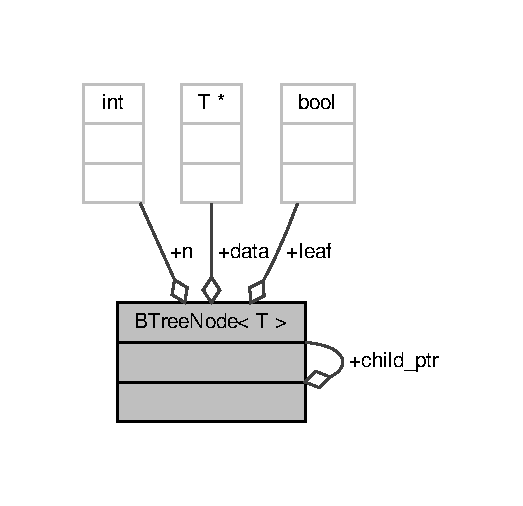
\includegraphics[width=251pt]{structBTreeNode__coll__graph}
\end{center}
\end{figure}
\subsection*{Public Attributes}
\begin{DoxyCompactItemize}
\item 
T $\ast$ \hyperlink{structBTreeNode_af877c66e47b110ed0f05e95351003531}{data}
\item 
\hyperlink{structBTreeNode}{B\+Tree\+Node} $\ast$$\ast$ \hyperlink{structBTreeNode_a723857b74be44c1921f17e177432a844}{child\+\_\+ptr}
\item 
bool \hyperlink{structBTreeNode_a8350f9ddcf6e2323413d9d061c382ea6}{leaf}
\item 
int \hyperlink{structBTreeNode_ac6993709a99bec1116e1c6dccc3c0f8a}{n}
\end{DoxyCompactItemize}


\subsection{Detailed Description}
\subsubsection*{template$<$typename T$>$\newline
struct B\+Tree\+Node$<$ T $>$}



Definition at line \hyperlink{BTree_8h_source_l00011}{11} of file \hyperlink{BTree_8h_source}{B\+Tree.\+h}.



\subsection{Member Data Documentation}
\mbox{\Hypertarget{structBTreeNode_a723857b74be44c1921f17e177432a844}\label{structBTreeNode_a723857b74be44c1921f17e177432a844}} 
\index{B\+Tree\+Node@{B\+Tree\+Node}!child\+\_\+ptr@{child\+\_\+ptr}}
\index{child\+\_\+ptr@{child\+\_\+ptr}!B\+Tree\+Node@{B\+Tree\+Node}}
\subsubsection{\texorpdfstring{child\+\_\+ptr}{child\_ptr}}
{\footnotesize\ttfamily template$<$typename T $>$ \\
\hyperlink{structBTreeNode}{B\+Tree\+Node}$\ast$$\ast$ \hyperlink{structBTreeNode}{B\+Tree\+Node}$<$ T $>$\+::child\+\_\+ptr}



Definition at line \hyperlink{BTree_8h_source_l00014}{14} of file \hyperlink{BTree_8h_source}{B\+Tree.\+h}.

\mbox{\Hypertarget{structBTreeNode_af877c66e47b110ed0f05e95351003531}\label{structBTreeNode_af877c66e47b110ed0f05e95351003531}} 
\index{B\+Tree\+Node@{B\+Tree\+Node}!data@{data}}
\index{data@{data}!B\+Tree\+Node@{B\+Tree\+Node}}
\subsubsection{\texorpdfstring{data}{data}}
{\footnotesize\ttfamily template$<$typename T $>$ \\
T$\ast$ \hyperlink{structBTreeNode}{B\+Tree\+Node}$<$ T $>$\+::data}



Definition at line \hyperlink{BTree_8h_source_l00013}{13} of file \hyperlink{BTree_8h_source}{B\+Tree.\+h}.

\mbox{\Hypertarget{structBTreeNode_a8350f9ddcf6e2323413d9d061c382ea6}\label{structBTreeNode_a8350f9ddcf6e2323413d9d061c382ea6}} 
\index{B\+Tree\+Node@{B\+Tree\+Node}!leaf@{leaf}}
\index{leaf@{leaf}!B\+Tree\+Node@{B\+Tree\+Node}}
\subsubsection{\texorpdfstring{leaf}{leaf}}
{\footnotesize\ttfamily template$<$typename T $>$ \\
bool \hyperlink{structBTreeNode}{B\+Tree\+Node}$<$ T $>$\+::leaf}



Definition at line \hyperlink{BTree_8h_source_l00015}{15} of file \hyperlink{BTree_8h_source}{B\+Tree.\+h}.

\mbox{\Hypertarget{structBTreeNode_ac6993709a99bec1116e1c6dccc3c0f8a}\label{structBTreeNode_ac6993709a99bec1116e1c6dccc3c0f8a}} 
\index{B\+Tree\+Node@{B\+Tree\+Node}!n@{n}}
\index{n@{n}!B\+Tree\+Node@{B\+Tree\+Node}}
\subsubsection{\texorpdfstring{n}{n}}
{\footnotesize\ttfamily template$<$typename T $>$ \\
int \hyperlink{structBTreeNode}{B\+Tree\+Node}$<$ T $>$\+::n}



Definition at line \hyperlink{BTree_8h_source_l00016}{16} of file \hyperlink{BTree_8h_source}{B\+Tree.\+h}.



The documentation for this struct was generated from the following file\+:\begin{DoxyCompactItemize}
\item 
\hyperlink{BTree_8h}{B\+Tree.\+h}\end{DoxyCompactItemize}

\hypertarget{classLinkedList}{}\section{Linked\+List$<$ Item\+Type $>$ Class Template Reference}
\label{classLinkedList}\index{Linked\+List$<$ Item\+Type $>$@{Linked\+List$<$ Item\+Type $>$}}


This is \hyperlink{classLinkedList}{Linked\+List} class creating a list of linked nodes.  




{\ttfamily \#include \char`\"{}Linked\+List.\+h\char`\"{}}



Inheritance diagram for Linked\+List$<$ Item\+Type $>$\+:\nopagebreak
\begin{figure}[H]
\begin{center}
\leavevmode
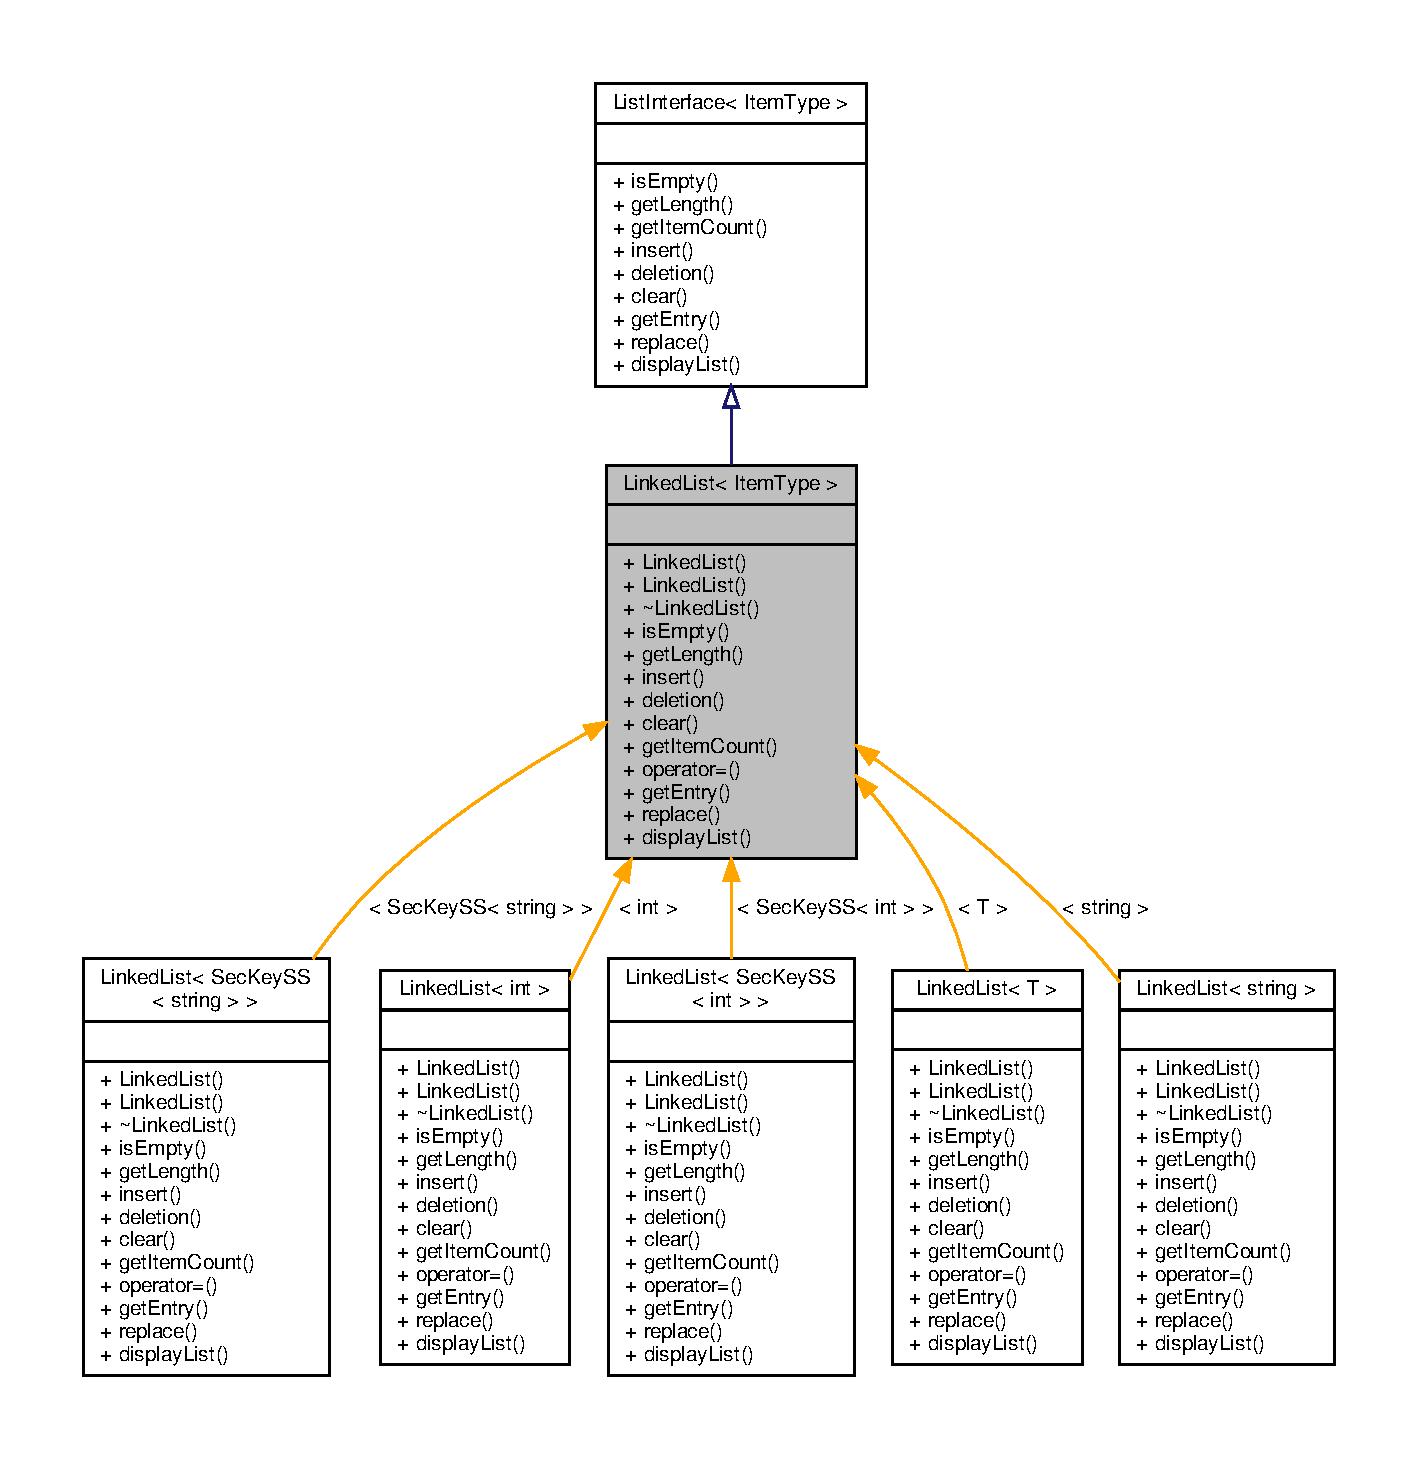
\includegraphics[width=350pt]{classLinkedList__inherit__graph}
\end{center}
\end{figure}


Collaboration diagram for Linked\+List$<$ Item\+Type $>$\+:\nopagebreak
\begin{figure}[H]
\begin{center}
\leavevmode
\includegraphics[width=210pt]{classLinkedList__coll__graph}
\end{center}
\end{figure}
\subsection*{Public Member Functions}
\begin{DoxyCompactItemize}
\item 
\hyperlink{classLinkedList_adf8d8164e06b6d358a36df7e53e814ee}{Linked\+List} ()
\begin{DoxyCompactList}\small\item\em \hyperlink{classLinkedList}{Linked\+List} default constructor. \end{DoxyCompactList}\item 
\hyperlink{classLinkedList_a6f1443c6120352f1f5b6bd3c0d95e41e}{Linked\+List} (const \hyperlink{classLinkedList}{Linked\+List}$<$ Item\+Type $>$ \&a\+List)
\begin{DoxyCompactList}\small\item\em \hyperlink{classLinkedList}{Linked\+List} constructor. \end{DoxyCompactList}\item 
virtual \hyperlink{classLinkedList_a66aee17d756fe0e002375897383c180b}{$\sim$\+Linked\+List} ()
\begin{DoxyCompactList}\small\item\em \hyperlink{classLinkedList}{Linked\+List} deconstructor. \end{DoxyCompactList}\item 
bool \hyperlink{classLinkedList_a008e916c3d51d28b4cc9c8cdf3e9d921}{is\+Empty} () const
\begin{DoxyCompactList}\small\item\em Memebr function to check if a \hyperlink{classLinkedList}{Linked\+List} is empty. \end{DoxyCompactList}\item 
int \hyperlink{classLinkedList_a61d045ef6008b494a1a516ecc992c0e7}{get\+Length} () const
\begin{DoxyCompactList}\small\item\em Member function to get the length of the \hyperlink{classLinkedList}{Linked\+List}. \end{DoxyCompactList}\item 
bool \hyperlink{classLinkedList_ae8a19375505e87e2e4fc0e9b5afe4d4d}{insert} (int new\+Position, const Item\+Type \&new\+Entry)
\begin{DoxyCompactList}\small\item\em Memebr function to insert a new item into a \hyperlink{classNode}{Node} of a \hyperlink{classLinkedList}{Linked\+List}. \end{DoxyCompactList}\item 
bool \hyperlink{classLinkedList_a7dc3cca217b45c6fe5d28c9d16b7bf9e}{deletion} (int position)
\begin{DoxyCompactList}\small\item\em Member function for deletion of a \hyperlink{classNode}{Node}. \end{DoxyCompactList}\item 
void \hyperlink{classLinkedList_a7d1d9cf83eef67b6c4d700a3cc5970e1}{clear} ()
\begin{DoxyCompactList}\small\item\em Memebr Fucntion to clear a \hyperlink{classLinkedList}{Linked\+List}. \end{DoxyCompactList}\item 
int \hyperlink{classLinkedList_afc6635f854f48f2f126cf3b60d845220}{get\+Item\+Count} () const
\begin{DoxyCompactList}\small\item\em Member function to get the item count. \end{DoxyCompactList}\item 
\hyperlink{classLinkedList}{Linked\+List}$<$ Item\+Type $>$ \& \hyperlink{classLinkedList_a25b0fba69e66b0fa409be992530029bc}{operator=} (const \hyperlink{classLinkedList}{Linked\+List}$<$ Item\+Type $>$ \&rhs)
\begin{DoxyCompactList}\small\item\em operator function = \end{DoxyCompactList}\item 
Item\+Type \hyperlink{classLinkedList_a341bfd7772c9d24d29eb7a7f3936915b}{get\+Entry} (int position) const
\begin{DoxyCompactList}\small\item\em Memebr function to get (return) an entry at a position. \end{DoxyCompactList}\item 
void \hyperlink{classLinkedList_a3035f880c50e7d8f68e67c093d4607ca}{replace} (int position, const Item\+Type \&new\+Entry)
\begin{DoxyCompactList}\small\item\em Member function to replace an item at a position. \end{DoxyCompactList}\item 
Item\+Type \hyperlink{classLinkedList_a65fb58d9f9b8af41e9569d1dc3200583}{display\+List} ()
\begin{DoxyCompactList}\small\item\em Member function to display the list. \end{DoxyCompactList}\end{DoxyCompactItemize}


\subsection{Detailed Description}
\subsubsection*{template$<$class Item\+Type$>$\newline
class Linked\+List$<$ Item\+Type $>$}

This is \hyperlink{classLinkedList}{Linked\+List} class creating a list of linked nodes. 

This class is to create a linked list of nodes. The nodes are of type template Item\+Type, item and a \hyperlink{classNode}{Node} pointer of item type, next. 

\subsection{Constructor \& Destructor Documentation}
\mbox{\Hypertarget{classLinkedList_adf8d8164e06b6d358a36df7e53e814ee}\label{classLinkedList_adf8d8164e06b6d358a36df7e53e814ee}} 
\index{Linked\+List@{Linked\+List}!Linked\+List@{Linked\+List}}
\index{Linked\+List@{Linked\+List}!Linked\+List@{Linked\+List}}
\subsubsection{\texorpdfstring{Linked\+List()}{LinkedList()}\hspace{0.1cm}{\footnotesize\ttfamily [1/2]}}
{\footnotesize\ttfamily template$<$class Item\+Type $>$ \\
\hyperlink{classLinkedList}{Linked\+List}$<$ Item\+Type $>$\+::\hyperlink{classLinkedList}{Linked\+List} (\begin{DoxyParamCaption}{ }\end{DoxyParamCaption})}



\hyperlink{classLinkedList}{Linked\+List} default constructor. 

Sets headptr to null and item\+Count to 0. \mbox{\Hypertarget{classLinkedList_a6f1443c6120352f1f5b6bd3c0d95e41e}\label{classLinkedList_a6f1443c6120352f1f5b6bd3c0d95e41e}} 
\index{Linked\+List@{Linked\+List}!Linked\+List@{Linked\+List}}
\index{Linked\+List@{Linked\+List}!Linked\+List@{Linked\+List}}
\subsubsection{\texorpdfstring{Linked\+List()}{LinkedList()}\hspace{0.1cm}{\footnotesize\ttfamily [2/2]}}
{\footnotesize\ttfamily template$<$class Item\+Type$>$ \\
\hyperlink{classLinkedList}{Linked\+List}$<$ Item\+Type $>$\+::\hyperlink{classLinkedList}{Linked\+List} (\begin{DoxyParamCaption}\item[{const \hyperlink{classLinkedList}{Linked\+List}$<$ Item\+Type $>$ \&}]{a\+List }\end{DoxyParamCaption})}



\hyperlink{classLinkedList}{Linked\+List} constructor. 

A copy constructor with one argumet passed, a\+List. 
\begin{DoxyParams}{Parameters}
{\em a\+Lsit} & a refrence to a list \\
\hline
\end{DoxyParams}
\mbox{\Hypertarget{classLinkedList_a66aee17d756fe0e002375897383c180b}\label{classLinkedList_a66aee17d756fe0e002375897383c180b}} 
\index{Linked\+List@{Linked\+List}!````~Linked\+List@{$\sim$\+Linked\+List}}
\index{````~Linked\+List@{$\sim$\+Linked\+List}!Linked\+List@{Linked\+List}}
\subsubsection{\texorpdfstring{$\sim$\+Linked\+List()}{~LinkedList()}}
{\footnotesize\ttfamily template$<$class Item\+Type $>$ \\
\hyperlink{classLinkedList}{Linked\+List}$<$ Item\+Type $>$\+::$\sim$\hyperlink{classLinkedList}{Linked\+List} (\begin{DoxyParamCaption}{ }\end{DoxyParamCaption})\hspace{0.3cm}{\ttfamily [virtual]}}



\hyperlink{classLinkedList}{Linked\+List} deconstructor. 

A deconstructor to clear a \hyperlink{classLinkedList}{Linked\+List} 

\subsection{Member Function Documentation}
\mbox{\Hypertarget{classLinkedList_a7d1d9cf83eef67b6c4d700a3cc5970e1}\label{classLinkedList_a7d1d9cf83eef67b6c4d700a3cc5970e1}} 
\index{Linked\+List@{Linked\+List}!clear@{clear}}
\index{clear@{clear}!Linked\+List@{Linked\+List}}
\subsubsection{\texorpdfstring{clear()}{clear()}}
{\footnotesize\ttfamily template$<$class Item\+Type $>$ \\
void \hyperlink{classLinkedList}{Linked\+List}$<$ Item\+Type $>$\+::clear (\begin{DoxyParamCaption}{ }\end{DoxyParamCaption})\hspace{0.3cm}{\ttfamily [virtual]}}



Memebr Fucntion to clear a \hyperlink{classLinkedList}{Linked\+List}. 

Removes 1 \hyperlink{classNode}{Node} at a time while the \hyperlink{classLinkedList}{Linked\+List} is not Empty 

Implements \hyperlink{classListInterface_adfda414908b645bdf19bcab8269168b7}{List\+Interface$<$ Item\+Type $>$}.

\mbox{\Hypertarget{classLinkedList_a7dc3cca217b45c6fe5d28c9d16b7bf9e}\label{classLinkedList_a7dc3cca217b45c6fe5d28c9d16b7bf9e}} 
\index{Linked\+List@{Linked\+List}!deletion@{deletion}}
\index{deletion@{deletion}!Linked\+List@{Linked\+List}}
\subsubsection{\texorpdfstring{deletion()}{deletion()}}
{\footnotesize\ttfamily template$<$class Item\+Type $>$ \\
bool \hyperlink{classLinkedList}{Linked\+List}$<$ Item\+Type $>$\+::deletion (\begin{DoxyParamCaption}\item[{int}]{position }\end{DoxyParamCaption})\hspace{0.3cm}{\ttfamily [virtual]}}



Member function for deletion of a \hyperlink{classNode}{Node}. 


\begin{DoxyParams}{Parameters}
{\em position} & the position of te \hyperlink{classNode}{Node} to be removed \\
\hline
\end{DoxyParams}
\begin{DoxyReturn}{Returns}
able\+To\+Remove returns true if the \hyperlink{classNode}{Node} is a valid \hyperlink{classNode}{Node}. 
\end{DoxyReturn}
\begin{DoxyPrecond}{Precondition}
To be a valid \hyperlink{classNode}{Node} to remove, psition $>$= 1 and position $<$= item\+Count 
\end{DoxyPrecond}


Implements \hyperlink{classListInterface_a68520ce2942ec716c745b1137c50a3c6}{List\+Interface$<$ Item\+Type $>$}.

\mbox{\Hypertarget{classLinkedList_a65fb58d9f9b8af41e9569d1dc3200583}\label{classLinkedList_a65fb58d9f9b8af41e9569d1dc3200583}} 
\index{Linked\+List@{Linked\+List}!display\+List@{display\+List}}
\index{display\+List@{display\+List}!Linked\+List@{Linked\+List}}
\subsubsection{\texorpdfstring{display\+List()}{displayList()}}
{\footnotesize\ttfamily template$<$class Item\+Type $>$ \\
Item\+Type \hyperlink{classLinkedList}{Linked\+List}$<$ Item\+Type $>$\+::display\+List (\begin{DoxyParamCaption}{ }\end{DoxyParamCaption})\hspace{0.3cm}{\ttfamily [virtual]}}



Member function to display the list. 

Displays the list by returing one \hyperlink{classNode}{Node} item at a time \begin{DoxyReturn}{Returns}
node\+Ptr-\/$>$get\+Item() an item at a node 
\end{DoxyReturn}


Implements \hyperlink{classListInterface_a2f2f533e962dd89111ee50b972dc28e7}{List\+Interface$<$ Item\+Type $>$}.

\mbox{\Hypertarget{classLinkedList_a341bfd7772c9d24d29eb7a7f3936915b}\label{classLinkedList_a341bfd7772c9d24d29eb7a7f3936915b}} 
\index{Linked\+List@{Linked\+List}!get\+Entry@{get\+Entry}}
\index{get\+Entry@{get\+Entry}!Linked\+List@{Linked\+List}}
\subsubsection{\texorpdfstring{get\+Entry()}{getEntry()}}
{\footnotesize\ttfamily template$<$class Item\+Type $>$ \\
Item\+Type \hyperlink{classLinkedList}{Linked\+List}$<$ Item\+Type $>$\+::get\+Entry (\begin{DoxyParamCaption}\item[{int}]{position }\end{DoxyParamCaption}) const\hspace{0.3cm}{\ttfamily [virtual]}}



Memebr function to get (return) an entry at a position. 


\begin{DoxyExceptions}{Exceptions}
{\em Precond\+Violated\+Excep} & if position $<$ 1 or position $>$ \hyperlink{classLinkedList_a61d045ef6008b494a1a516ecc992c0e7}{get\+Length()}.\\
\hline
\end{DoxyExceptions}

\begin{DoxyParams}{Parameters}
{\em position} & the position of a \hyperlink{classNode}{Node} to return an\+Item \\
\hline
\end{DoxyParams}
\begin{DoxyReturn}{Returns}
node\+Ptr-\/$>$get\+Item() an item at the position, position. 
\end{DoxyReturn}
\begin{DoxyPrecond}{Precondition}
position $>$ 0 and position $<$= item\+Count 
\end{DoxyPrecond}


Implements \hyperlink{classListInterface_a86987f69e5056d287212ede41db1956a}{List\+Interface$<$ Item\+Type $>$}.

\mbox{\Hypertarget{classLinkedList_afc6635f854f48f2f126cf3b60d845220}\label{classLinkedList_afc6635f854f48f2f126cf3b60d845220}} 
\index{Linked\+List@{Linked\+List}!get\+Item\+Count@{get\+Item\+Count}}
\index{get\+Item\+Count@{get\+Item\+Count}!Linked\+List@{Linked\+List}}
\subsubsection{\texorpdfstring{get\+Item\+Count()}{getItemCount()}}
{\footnotesize\ttfamily template$<$class Item\+Type $>$ \\
int \hyperlink{classLinkedList}{Linked\+List}$<$ Item\+Type $>$\+::get\+Item\+Count (\begin{DoxyParamCaption}{ }\end{DoxyParamCaption}) const\hspace{0.3cm}{\ttfamily [virtual]}}



Member function to get the item count. 

/return item\+Count the count of items in the \hyperlink{classLinkedList}{Linked\+List} 

Implements \hyperlink{classListInterface_a3e085e6ea9c5dc3e8007010cd889159c}{List\+Interface$<$ Item\+Type $>$}.

\mbox{\Hypertarget{classLinkedList_a61d045ef6008b494a1a516ecc992c0e7}\label{classLinkedList_a61d045ef6008b494a1a516ecc992c0e7}} 
\index{Linked\+List@{Linked\+List}!get\+Length@{get\+Length}}
\index{get\+Length@{get\+Length}!Linked\+List@{Linked\+List}}
\subsubsection{\texorpdfstring{get\+Length()}{getLength()}}
{\footnotesize\ttfamily template$<$class Item\+Type $>$ \\
int \hyperlink{classLinkedList}{Linked\+List}$<$ Item\+Type $>$\+::get\+Length (\begin{DoxyParamCaption}{ }\end{DoxyParamCaption}) const\hspace{0.3cm}{\ttfamily [virtual]}}



Member function to get the length of the \hyperlink{classLinkedList}{Linked\+List}. 

\begin{DoxyReturn}{Returns}
item\+Count the length (count of items) of the \hyperlink{classLinkedList}{Linked\+List} 
\end{DoxyReturn}


Implements \hyperlink{classListInterface_afc85695d4137f1e29ff02e179c9f3221}{List\+Interface$<$ Item\+Type $>$}.

\mbox{\Hypertarget{classLinkedList_ae8a19375505e87e2e4fc0e9b5afe4d4d}\label{classLinkedList_ae8a19375505e87e2e4fc0e9b5afe4d4d}} 
\index{Linked\+List@{Linked\+List}!insert@{insert}}
\index{insert@{insert}!Linked\+List@{Linked\+List}}
\subsubsection{\texorpdfstring{insert()}{insert()}}
{\footnotesize\ttfamily template$<$class Item\+Type$>$ \\
bool \hyperlink{classLinkedList}{Linked\+List}$<$ Item\+Type $>$\+::insert (\begin{DoxyParamCaption}\item[{int}]{new\+Position,  }\item[{const Item\+Type \&}]{new\+Entry }\end{DoxyParamCaption})\hspace{0.3cm}{\ttfamily [virtual]}}



Memebr function to insert a new item into a \hyperlink{classNode}{Node} of a \hyperlink{classLinkedList}{Linked\+List}. 


\begin{DoxyParams}{Parameters}
{\em new\+Position} & a node position to insert a item into \\
\hline
{\em new\+Entry} & a reference to an item of item\+Type to be inserted into the \hyperlink{classNode}{Node}. \\
\hline
\end{DoxyParams}
\begin{DoxyReturn}{Returns}
able\+To\+Insert if new\+Entry can be inserted into the \hyperlink{classNode}{Node} at new\+Position 
\end{DoxyReturn}
\begin{DoxyPrecond}{Precondition}
new\+Position $>$= 1 

new\+Position $<$= item\+Count + 1 
\end{DoxyPrecond}


Implements \hyperlink{classListInterface_a5b2f86954a86172699a3495982c38e77}{List\+Interface$<$ Item\+Type $>$}.

\mbox{\Hypertarget{classLinkedList_a008e916c3d51d28b4cc9c8cdf3e9d921}\label{classLinkedList_a008e916c3d51d28b4cc9c8cdf3e9d921}} 
\index{Linked\+List@{Linked\+List}!is\+Empty@{is\+Empty}}
\index{is\+Empty@{is\+Empty}!Linked\+List@{Linked\+List}}
\subsubsection{\texorpdfstring{is\+Empty()}{isEmpty()}}
{\footnotesize\ttfamily template$<$class Item\+Type $>$ \\
bool \hyperlink{classLinkedList}{Linked\+List}$<$ Item\+Type $>$\+::is\+Empty (\begin{DoxyParamCaption}{ }\end{DoxyParamCaption}) const\hspace{0.3cm}{\ttfamily [virtual]}}



Memebr function to check if a \hyperlink{classLinkedList}{Linked\+List} is empty. 

Checks and returns a boolean value if the list is true or not \begin{DoxyReturn}{Returns}
item\+Count == 0 returns 1 if the \hyperlink{classLinkedList}{Linked\+List} is empty, 0 otherwise. 
\end{DoxyReturn}


Implements \hyperlink{classListInterface_a924f91e7f81d7dcd3fda79bbcc671394}{List\+Interface$<$ Item\+Type $>$}.

\mbox{\Hypertarget{classLinkedList_a25b0fba69e66b0fa409be992530029bc}\label{classLinkedList_a25b0fba69e66b0fa409be992530029bc}} 
\index{Linked\+List@{Linked\+List}!operator=@{operator=}}
\index{operator=@{operator=}!Linked\+List@{Linked\+List}}
\subsubsection{\texorpdfstring{operator=()}{operator=()}}
{\footnotesize\ttfamily template$<$class Item\+Type$>$ \\
\hyperlink{classLinkedList}{Linked\+List}$<$ Item\+Type $>$ \& \hyperlink{classLinkedList}{Linked\+List}$<$ Item\+Type $>$\+::operator= (\begin{DoxyParamCaption}\item[{const \hyperlink{classLinkedList}{Linked\+List}$<$ Item\+Type $>$ \&}]{rhs }\end{DoxyParamCaption})}



operator function = 


\begin{DoxyParams}{Parameters}
{\em rhs} & referance to a \hyperlink{classLinkedList}{Linked\+List} \\
\hline
\end{DoxyParams}
\begin{DoxyReturn}{Returns}
$\ast$this a pointer to the \hyperlink{classLinkedList}{Linked\+List} 
\end{DoxyReturn}
\mbox{\Hypertarget{classLinkedList_a3035f880c50e7d8f68e67c093d4607ca}\label{classLinkedList_a3035f880c50e7d8f68e67c093d4607ca}} 
\index{Linked\+List@{Linked\+List}!replace@{replace}}
\index{replace@{replace}!Linked\+List@{Linked\+List}}
\subsubsection{\texorpdfstring{replace()}{replace()}}
{\footnotesize\ttfamily template$<$class Item\+Type$>$ \\
void \hyperlink{classLinkedList}{Linked\+List}$<$ Item\+Type $>$\+::replace (\begin{DoxyParamCaption}\item[{int}]{position,  }\item[{const Item\+Type \&}]{new\+Entry }\end{DoxyParamCaption})\hspace{0.3cm}{\ttfamily [virtual]}}



Member function to replace an item at a position. 


\begin{DoxyExceptions}{Exceptions}
{\em Precond\+Violated\+Excep} & if position $<$ 1 or position $>$ \hyperlink{classLinkedList_a61d045ef6008b494a1a516ecc992c0e7}{get\+Length()}.\\
\hline
\end{DoxyExceptions}

\begin{DoxyParams}{Parameters}
{\em position} & the position of the \hyperlink{classNode}{Node} whos item will be replaced \\
\hline
{\em new\+Entry} & the new entery to replace the old entry of a \hyperlink{classNode}{Node} \\
\hline
\end{DoxyParams}


Implements \hyperlink{classListInterface_aae877a56b7b9f5f526c37a00e234fad1}{List\+Interface$<$ Item\+Type $>$}.



The documentation for this class was generated from the following files\+:\begin{DoxyCompactItemize}
\item 
\hyperlink{LinkedList_8h}{Linked\+List.\+h}\item 
\hyperlink{LinkedList_8cpp}{Linked\+List.\+cpp}\end{DoxyCompactItemize}

\hypertarget{classListInterface}{}\section{List\+Interface$<$ Item\+Type $>$ Class Template Reference}
\label{classListInterface}\index{List\+Interface$<$ Item\+Type $>$@{List\+Interface$<$ Item\+Type $>$}}


{\ttfamily \#include $<$List\+Interface.\+h$>$}



Inheritance diagram for List\+Interface$<$ Item\+Type $>$\+:\nopagebreak
\begin{figure}[H]
\begin{center}
\leavevmode
\includegraphics[width=350pt]{classListInterface__inherit__graph}
\end{center}
\end{figure}


Collaboration diagram for List\+Interface$<$ Item\+Type $>$\+:\nopagebreak
\begin{figure}[H]
\begin{center}
\leavevmode
\includegraphics[width=210pt]{classListInterface__coll__graph}
\end{center}
\end{figure}
\subsection*{Public Member Functions}
\begin{DoxyCompactItemize}
\item 
virtual bool \hyperlink{classListInterface_a924f91e7f81d7dcd3fda79bbcc671394}{is\+Empty} () const =0
\item 
virtual int \hyperlink{classListInterface_afc85695d4137f1e29ff02e179c9f3221}{get\+Length} () const =0
\item 
virtual int \hyperlink{classListInterface_a3e085e6ea9c5dc3e8007010cd889159c}{get\+Item\+Count} () const =0
\item 
virtual bool \hyperlink{classListInterface_a5b2f86954a86172699a3495982c38e77}{insert} (int new\+Position, const Item\+Type \&new\+Entry)=0
\item 
virtual bool \hyperlink{classListInterface_a68520ce2942ec716c745b1137c50a3c6}{deletion} (int position)=0
\item 
virtual void \hyperlink{classListInterface_adfda414908b645bdf19bcab8269168b7}{clear} ()=0
\item 
virtual Item\+Type \hyperlink{classListInterface_a86987f69e5056d287212ede41db1956a}{get\+Entry} (int position) const =0
\item 
virtual void \hyperlink{classListInterface_aae877a56b7b9f5f526c37a00e234fad1}{replace} (int position, const Item\+Type \&new\+Entry)=0
\item 
virtual Item\+Type \hyperlink{classListInterface_a2f2f533e962dd89111ee50b972dc28e7}{display\+List} ()=0
\end{DoxyCompactItemize}


\subsection{Member Function Documentation}
\mbox{\Hypertarget{classListInterface_adfda414908b645bdf19bcab8269168b7}\label{classListInterface_adfda414908b645bdf19bcab8269168b7}} 
\index{List\+Interface@{List\+Interface}!clear@{clear}}
\index{clear@{clear}!List\+Interface@{List\+Interface}}
\subsubsection{\texorpdfstring{clear()}{clear()}}
{\footnotesize\ttfamily template$<$class Item\+Type$>$ \\
virtual void \hyperlink{classListInterface}{List\+Interface}$<$ Item\+Type $>$\+::clear (\begin{DoxyParamCaption}{ }\end{DoxyParamCaption})\hspace{0.3cm}{\ttfamily [pure virtual]}}

Removes all entries from this list. \begin{DoxyPostcond}{Postcondition}
List contains no entries and the count of items is 0. 
\end{DoxyPostcond}


Implemented in \hyperlink{classLinkedList_a7d1d9cf83eef67b6c4d700a3cc5970e1}{Linked\+List$<$ Item\+Type $>$}, \hyperlink{classLinkedList_a7d1d9cf83eef67b6c4d700a3cc5970e1}{Linked\+List$<$ Sec\+Key\+S\+S$<$ string $>$ $>$}, \hyperlink{classLinkedList_a7d1d9cf83eef67b6c4d700a3cc5970e1}{Linked\+List$<$ int $>$}, \hyperlink{classLinkedList_a7d1d9cf83eef67b6c4d700a3cc5970e1}{Linked\+List$<$ Sec\+Key\+S\+S$<$ int $>$ $>$}, \hyperlink{classLinkedList_a7d1d9cf83eef67b6c4d700a3cc5970e1}{Linked\+List$<$ T $>$}, and \hyperlink{classLinkedList_a7d1d9cf83eef67b6c4d700a3cc5970e1}{Linked\+List$<$ string $>$}.

\mbox{\Hypertarget{classListInterface_a68520ce2942ec716c745b1137c50a3c6}\label{classListInterface_a68520ce2942ec716c745b1137c50a3c6}} 
\index{List\+Interface@{List\+Interface}!deletion@{deletion}}
\index{deletion@{deletion}!List\+Interface@{List\+Interface}}
\subsubsection{\texorpdfstring{deletion()}{deletion()}}
{\footnotesize\ttfamily template$<$class Item\+Type$>$ \\
virtual bool \hyperlink{classListInterface}{List\+Interface}$<$ Item\+Type $>$\+::deletion (\begin{DoxyParamCaption}\item[{int}]{position }\end{DoxyParamCaption})\hspace{0.3cm}{\ttfamily [pure virtual]}}

Removes the entry at a given position from this list. \begin{DoxyPrecond}{Precondition}
None. 
\end{DoxyPrecond}
\begin{DoxyPostcond}{Postcondition}
If 1 $<$= position $<$= \hyperlink{classListInterface_afc85695d4137f1e29ff02e179c9f3221}{get\+Length()} and the removal is successful, the entry at the given position in the list is removed, other items are renumbered accordingly, and the returned value is true. 
\end{DoxyPostcond}

\begin{DoxyParams}{Parameters}
{\em position} & The list position of the entry to remove. \\
\hline
\end{DoxyParams}
\begin{DoxyReturn}{Returns}
True if removal is successful, or false if not. 
\end{DoxyReturn}


Implemented in \hyperlink{classLinkedList_a7dc3cca217b45c6fe5d28c9d16b7bf9e}{Linked\+List$<$ Item\+Type $>$}, \hyperlink{classLinkedList_a7dc3cca217b45c6fe5d28c9d16b7bf9e}{Linked\+List$<$ Sec\+Key\+S\+S$<$ string $>$ $>$}, \hyperlink{classLinkedList_a7dc3cca217b45c6fe5d28c9d16b7bf9e}{Linked\+List$<$ int $>$}, \hyperlink{classLinkedList_a7dc3cca217b45c6fe5d28c9d16b7bf9e}{Linked\+List$<$ Sec\+Key\+S\+S$<$ int $>$ $>$}, \hyperlink{classLinkedList_a7dc3cca217b45c6fe5d28c9d16b7bf9e}{Linked\+List$<$ T $>$}, and \hyperlink{classLinkedList_a7dc3cca217b45c6fe5d28c9d16b7bf9e}{Linked\+List$<$ string $>$}.

\mbox{\Hypertarget{classListInterface_a2f2f533e962dd89111ee50b972dc28e7}\label{classListInterface_a2f2f533e962dd89111ee50b972dc28e7}} 
\index{List\+Interface@{List\+Interface}!display\+List@{display\+List}}
\index{display\+List@{display\+List}!List\+Interface@{List\+Interface}}
\subsubsection{\texorpdfstring{display\+List()}{displayList()}}
{\footnotesize\ttfamily template$<$class Item\+Type$>$ \\
virtual Item\+Type \hyperlink{classListInterface}{List\+Interface}$<$ Item\+Type $>$\+::display\+List (\begin{DoxyParamCaption}{ }\end{DoxyParamCaption})\hspace{0.3cm}{\ttfamily [pure virtual]}}



Implemented in \hyperlink{classLinkedList_a65fb58d9f9b8af41e9569d1dc3200583}{Linked\+List$<$ Item\+Type $>$}, \hyperlink{classLinkedList_a65fb58d9f9b8af41e9569d1dc3200583}{Linked\+List$<$ Sec\+Key\+S\+S$<$ string $>$ $>$}, \hyperlink{classLinkedList_a65fb58d9f9b8af41e9569d1dc3200583}{Linked\+List$<$ int $>$}, \hyperlink{classLinkedList_a65fb58d9f9b8af41e9569d1dc3200583}{Linked\+List$<$ Sec\+Key\+S\+S$<$ int $>$ $>$}, \hyperlink{classLinkedList_a65fb58d9f9b8af41e9569d1dc3200583}{Linked\+List$<$ T $>$}, and \hyperlink{classLinkedList_a65fb58d9f9b8af41e9569d1dc3200583}{Linked\+List$<$ string $>$}.

\mbox{\Hypertarget{classListInterface_a86987f69e5056d287212ede41db1956a}\label{classListInterface_a86987f69e5056d287212ede41db1956a}} 
\index{List\+Interface@{List\+Interface}!get\+Entry@{get\+Entry}}
\index{get\+Entry@{get\+Entry}!List\+Interface@{List\+Interface}}
\subsubsection{\texorpdfstring{get\+Entry()}{getEntry()}}
{\footnotesize\ttfamily template$<$class Item\+Type$>$ \\
virtual Item\+Type \hyperlink{classListInterface}{List\+Interface}$<$ Item\+Type $>$\+::get\+Entry (\begin{DoxyParamCaption}\item[{int}]{position }\end{DoxyParamCaption}) const\hspace{0.3cm}{\ttfamily [pure virtual]}}

Gets the entry at the given position in this list. \begin{DoxyPrecond}{Precondition}
1 $<$= position $<$= \hyperlink{classListInterface_afc85695d4137f1e29ff02e179c9f3221}{get\+Length()}. 
\end{DoxyPrecond}
\begin{DoxyPostcond}{Postcondition}
The desired entry has been returned. 
\end{DoxyPostcond}

\begin{DoxyParams}{Parameters}
{\em position} & The list position of the desired entry. \\
\hline
\end{DoxyParams}
\begin{DoxyReturn}{Returns}
The entry at the given position. 
\end{DoxyReturn}


Implemented in \hyperlink{classLinkedList_a341bfd7772c9d24d29eb7a7f3936915b}{Linked\+List$<$ Item\+Type $>$}, \hyperlink{classLinkedList_a341bfd7772c9d24d29eb7a7f3936915b}{Linked\+List$<$ Sec\+Key\+S\+S$<$ string $>$ $>$}, \hyperlink{classLinkedList_a341bfd7772c9d24d29eb7a7f3936915b}{Linked\+List$<$ int $>$}, \hyperlink{classLinkedList_a341bfd7772c9d24d29eb7a7f3936915b}{Linked\+List$<$ Sec\+Key\+S\+S$<$ int $>$ $>$}, \hyperlink{classLinkedList_a341bfd7772c9d24d29eb7a7f3936915b}{Linked\+List$<$ T $>$}, and \hyperlink{classLinkedList_a341bfd7772c9d24d29eb7a7f3936915b}{Linked\+List$<$ string $>$}.

\mbox{\Hypertarget{classListInterface_a3e085e6ea9c5dc3e8007010cd889159c}\label{classListInterface_a3e085e6ea9c5dc3e8007010cd889159c}} 
\index{List\+Interface@{List\+Interface}!get\+Item\+Count@{get\+Item\+Count}}
\index{get\+Item\+Count@{get\+Item\+Count}!List\+Interface@{List\+Interface}}
\subsubsection{\texorpdfstring{get\+Item\+Count()}{getItemCount()}}
{\footnotesize\ttfamily template$<$class Item\+Type$>$ \\
virtual int \hyperlink{classListInterface}{List\+Interface}$<$ Item\+Type $>$\+::get\+Item\+Count (\begin{DoxyParamCaption}{ }\end{DoxyParamCaption}) const\hspace{0.3cm}{\ttfamily [pure virtual]}}



Implemented in \hyperlink{classLinkedList_afc6635f854f48f2f126cf3b60d845220}{Linked\+List$<$ Item\+Type $>$}, \hyperlink{classLinkedList_afc6635f854f48f2f126cf3b60d845220}{Linked\+List$<$ Sec\+Key\+S\+S$<$ string $>$ $>$}, \hyperlink{classLinkedList_afc6635f854f48f2f126cf3b60d845220}{Linked\+List$<$ int $>$}, \hyperlink{classLinkedList_afc6635f854f48f2f126cf3b60d845220}{Linked\+List$<$ Sec\+Key\+S\+S$<$ int $>$ $>$}, \hyperlink{classLinkedList_afc6635f854f48f2f126cf3b60d845220}{Linked\+List$<$ T $>$}, and \hyperlink{classLinkedList_afc6635f854f48f2f126cf3b60d845220}{Linked\+List$<$ string $>$}.

\mbox{\Hypertarget{classListInterface_afc85695d4137f1e29ff02e179c9f3221}\label{classListInterface_afc85695d4137f1e29ff02e179c9f3221}} 
\index{List\+Interface@{List\+Interface}!get\+Length@{get\+Length}}
\index{get\+Length@{get\+Length}!List\+Interface@{List\+Interface}}
\subsubsection{\texorpdfstring{get\+Length()}{getLength()}}
{\footnotesize\ttfamily template$<$class Item\+Type$>$ \\
virtual int \hyperlink{classListInterface}{List\+Interface}$<$ Item\+Type $>$\+::get\+Length (\begin{DoxyParamCaption}{ }\end{DoxyParamCaption}) const\hspace{0.3cm}{\ttfamily [pure virtual]}}

Gets the current number of entries in this list. \begin{DoxyReturn}{Returns}
The integer number of entries currently in the list. 
\end{DoxyReturn}


Implemented in \hyperlink{classLinkedList_a61d045ef6008b494a1a516ecc992c0e7}{Linked\+List$<$ Item\+Type $>$}, \hyperlink{classLinkedList_a61d045ef6008b494a1a516ecc992c0e7}{Linked\+List$<$ Sec\+Key\+S\+S$<$ string $>$ $>$}, \hyperlink{classLinkedList_a61d045ef6008b494a1a516ecc992c0e7}{Linked\+List$<$ int $>$}, \hyperlink{classLinkedList_a61d045ef6008b494a1a516ecc992c0e7}{Linked\+List$<$ Sec\+Key\+S\+S$<$ int $>$ $>$}, \hyperlink{classLinkedList_a61d045ef6008b494a1a516ecc992c0e7}{Linked\+List$<$ T $>$}, and \hyperlink{classLinkedList_a61d045ef6008b494a1a516ecc992c0e7}{Linked\+List$<$ string $>$}.

\mbox{\Hypertarget{classListInterface_a5b2f86954a86172699a3495982c38e77}\label{classListInterface_a5b2f86954a86172699a3495982c38e77}} 
\index{List\+Interface@{List\+Interface}!insert@{insert}}
\index{insert@{insert}!List\+Interface@{List\+Interface}}
\subsubsection{\texorpdfstring{insert()}{insert()}}
{\footnotesize\ttfamily template$<$class Item\+Type$>$ \\
virtual bool \hyperlink{classListInterface}{List\+Interface}$<$ Item\+Type $>$\+::insert (\begin{DoxyParamCaption}\item[{int}]{new\+Position,  }\item[{const Item\+Type \&}]{new\+Entry }\end{DoxyParamCaption})\hspace{0.3cm}{\ttfamily [pure virtual]}}

Inserts an entry into this list at a given position. \begin{DoxyPrecond}{Precondition}
None. 
\end{DoxyPrecond}
\begin{DoxyPostcond}{Postcondition}
If 1 $<$= position $<$= \hyperlink{classListInterface_afc85695d4137f1e29ff02e179c9f3221}{get\+Length()} + 1 and the insertion is successful, new\+Entry is at the given position in the list, other entries are renumbered accordingly, and the returned value is true. 
\end{DoxyPostcond}

\begin{DoxyParams}{Parameters}
{\em new\+Position} & The list position at which to insert new\+Entry. \\
\hline
{\em new\+Entry} & The entry to insert into the list. \\
\hline
\end{DoxyParams}
\begin{DoxyReturn}{Returns}
True if insertion is successful, or false if not. 
\end{DoxyReturn}


Implemented in \hyperlink{classLinkedList_ae8a19375505e87e2e4fc0e9b5afe4d4d}{Linked\+List$<$ Item\+Type $>$}, \hyperlink{classLinkedList_ae8a19375505e87e2e4fc0e9b5afe4d4d}{Linked\+List$<$ Sec\+Key\+S\+S$<$ string $>$ $>$}, \hyperlink{classLinkedList_ae8a19375505e87e2e4fc0e9b5afe4d4d}{Linked\+List$<$ int $>$}, \hyperlink{classLinkedList_ae8a19375505e87e2e4fc0e9b5afe4d4d}{Linked\+List$<$ Sec\+Key\+S\+S$<$ int $>$ $>$}, \hyperlink{classLinkedList_ae8a19375505e87e2e4fc0e9b5afe4d4d}{Linked\+List$<$ T $>$}, and \hyperlink{classLinkedList_ae8a19375505e87e2e4fc0e9b5afe4d4d}{Linked\+List$<$ string $>$}.

\mbox{\Hypertarget{classListInterface_a924f91e7f81d7dcd3fda79bbcc671394}\label{classListInterface_a924f91e7f81d7dcd3fda79bbcc671394}} 
\index{List\+Interface@{List\+Interface}!is\+Empty@{is\+Empty}}
\index{is\+Empty@{is\+Empty}!List\+Interface@{List\+Interface}}
\subsubsection{\texorpdfstring{is\+Empty()}{isEmpty()}}
{\footnotesize\ttfamily template$<$class Item\+Type$>$ \\
virtual bool \hyperlink{classListInterface}{List\+Interface}$<$ Item\+Type $>$\+::is\+Empty (\begin{DoxyParamCaption}{ }\end{DoxyParamCaption}) const\hspace{0.3cm}{\ttfamily [pure virtual]}}

Sees whether this list is empty. \begin{DoxyReturn}{Returns}
True if the list is empty; otherwise returns false. 
\end{DoxyReturn}


Implemented in \hyperlink{classLinkedList_a008e916c3d51d28b4cc9c8cdf3e9d921}{Linked\+List$<$ Item\+Type $>$}, \hyperlink{classLinkedList_a008e916c3d51d28b4cc9c8cdf3e9d921}{Linked\+List$<$ Sec\+Key\+S\+S$<$ string $>$ $>$}, \hyperlink{classLinkedList_a008e916c3d51d28b4cc9c8cdf3e9d921}{Linked\+List$<$ int $>$}, \hyperlink{classLinkedList_a008e916c3d51d28b4cc9c8cdf3e9d921}{Linked\+List$<$ Sec\+Key\+S\+S$<$ int $>$ $>$}, \hyperlink{classLinkedList_a008e916c3d51d28b4cc9c8cdf3e9d921}{Linked\+List$<$ T $>$}, and \hyperlink{classLinkedList_a008e916c3d51d28b4cc9c8cdf3e9d921}{Linked\+List$<$ string $>$}.

\mbox{\Hypertarget{classListInterface_aae877a56b7b9f5f526c37a00e234fad1}\label{classListInterface_aae877a56b7b9f5f526c37a00e234fad1}} 
\index{List\+Interface@{List\+Interface}!replace@{replace}}
\index{replace@{replace}!List\+Interface@{List\+Interface}}
\subsubsection{\texorpdfstring{replace()}{replace()}}
{\footnotesize\ttfamily template$<$class Item\+Type$>$ \\
virtual void \hyperlink{classListInterface}{List\+Interface}$<$ Item\+Type $>$\+::replace (\begin{DoxyParamCaption}\item[{int}]{position,  }\item[{const Item\+Type \&}]{new\+Entry }\end{DoxyParamCaption})\hspace{0.3cm}{\ttfamily [pure virtual]}}

Replaces the entry at the given position in this list. \begin{DoxyPrecond}{Precondition}
1 $<$= position $<$= \hyperlink{classListInterface_afc85695d4137f1e29ff02e179c9f3221}{get\+Length()}. 
\end{DoxyPrecond}
\begin{DoxyPostcond}{Postcondition}
The entry at the given position is new\+Entry. 
\end{DoxyPostcond}

\begin{DoxyParams}{Parameters}
{\em position} & The list position of the entry to replace. \\
\hline
{\em new\+Entry} & The replacement entry. \\
\hline
\end{DoxyParams}


Implemented in \hyperlink{classLinkedList_a3035f880c50e7d8f68e67c093d4607ca}{Linked\+List$<$ Item\+Type $>$}, \hyperlink{classLinkedList_a3035f880c50e7d8f68e67c093d4607ca}{Linked\+List$<$ Sec\+Key\+S\+S$<$ string $>$ $>$}, \hyperlink{classLinkedList_a3035f880c50e7d8f68e67c093d4607ca}{Linked\+List$<$ int $>$}, \hyperlink{classLinkedList_a3035f880c50e7d8f68e67c093d4607ca}{Linked\+List$<$ Sec\+Key\+S\+S$<$ int $>$ $>$}, \hyperlink{classLinkedList_a3035f880c50e7d8f68e67c093d4607ca}{Linked\+List$<$ T $>$}, and \hyperlink{classLinkedList_a3035f880c50e7d8f68e67c093d4607ca}{Linked\+List$<$ string $>$}.



The documentation for this class was generated from the following file\+:\begin{DoxyCompactItemize}
\item 
\hyperlink{ListInterface_8h}{List\+Interface.\+h}\end{DoxyCompactItemize}

\hypertarget{classNode}{}\section{Node$<$ Item\+Type $>$ Class Template Reference}
\label{classNode}\index{Node$<$ Item\+Type $>$@{Node$<$ Item\+Type $>$}}


This is \hyperlink{classNode}{Node} class for linked list.  




{\ttfamily \#include \char`\"{}Node.\+h\char`\"{}}



Inheritance diagram for Node$<$ Item\+Type $>$\+:\nopagebreak
\begin{figure}[H]
\begin{center}
\leavevmode
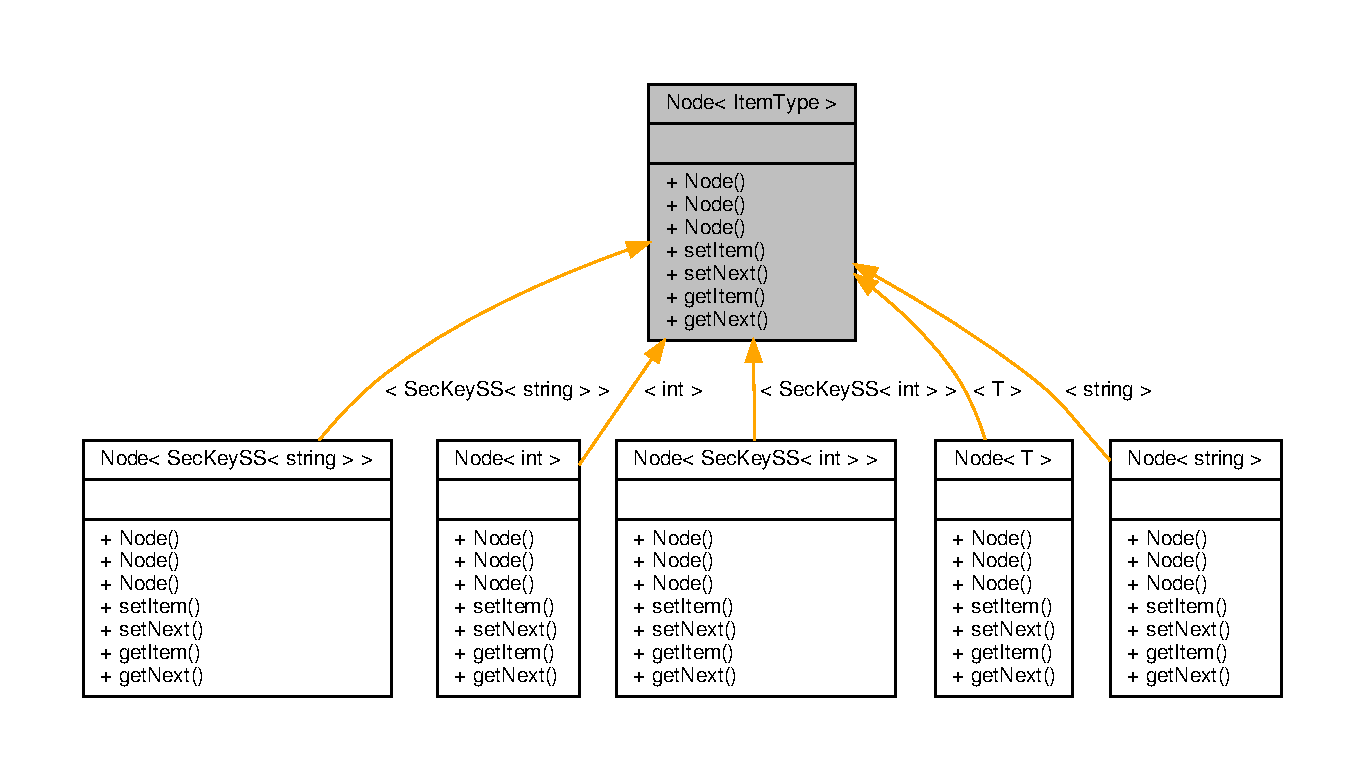
\includegraphics[width=350pt]{classNode__inherit__graph}
\end{center}
\end{figure}


Collaboration diagram for Node$<$ Item\+Type $>$\+:\nopagebreak
\begin{figure}[H]
\begin{center}
\leavevmode
\includegraphics[width=179pt]{classNode__coll__graph}
\end{center}
\end{figure}
\subsection*{Public Member Functions}
\begin{DoxyCompactItemize}
\item 
\hyperlink{classNode_a627e94f4fba0e73c546e0fb2a7266f36}{Node} ()
\begin{DoxyCompactList}\small\item\em \hyperlink{classNode}{Node} default constructor. \end{DoxyCompactList}\item 
\hyperlink{classNode_a0288598fcb0244739ce95099c26250ae}{Node} (const Item\+Type \&an\+Item)
\begin{DoxyCompactList}\small\item\em \hyperlink{classNode}{Node} constructor. \end{DoxyCompactList}\item 
\hyperlink{classNode_adf98d3f9b7227622cb5a0fdd7e8f0b18}{Node} (const Item\+Type \&an\+Item, \hyperlink{classNode}{Node}$<$ Item\+Type $>$ $\ast$next\+Node\+Ptr)
\begin{DoxyCompactList}\small\item\em \hyperlink{classNode}{Node} constructor. \end{DoxyCompactList}\item 
void \hyperlink{classNode_ab4ceecdecc5df799011de486b9f54974}{set\+Item} (const Item\+Type \&an\+Item)
\begin{DoxyCompactList}\small\item\em Member function taking one argument to set the memebr item. \end{DoxyCompactList}\item 
void \hyperlink{classNode_a01c1a66d4e39f5b149e090413deb4633}{set\+Next} (\hyperlink{classNode}{Node}$<$ Item\+Type $>$ $\ast$next\+Node\+Ptr)
\begin{DoxyCompactList}\small\item\em Member function taking one argument, a pointer to a \hyperlink{classNode}{Node}. \end{DoxyCompactList}\item 
Item\+Type \hyperlink{classNode_a6c08caef312b6f2f69b5e090cf047514}{get\+Item} () const
\begin{DoxyCompactList}\small\item\em Member function returning an item. \end{DoxyCompactList}\item 
\hyperlink{classNode}{Node}$<$ Item\+Type $>$ $\ast$ \hyperlink{classNode_a3eb0c96e03a3fd46ea1cff4c305bbedd}{get\+Next} () const
\begin{DoxyCompactList}\small\item\em Memebr funtion to get the pointer to the next \hyperlink{classNode}{Node}. \end{DoxyCompactList}\end{DoxyCompactItemize}


\subsection{Detailed Description}
\subsubsection*{template$<$class Item\+Type$>$\newline
class Node$<$ Item\+Type $>$}

This is \hyperlink{classNode}{Node} class for linked list. 

This class is to create a node that is used in linked list class. The \hyperlink{classNode}{Node} will store a template Item\+Type, item and a \hyperlink{classNode}{Node} pointer of item type, next. 

\subsection{Constructor \& Destructor Documentation}
\mbox{\Hypertarget{classNode_a627e94f4fba0e73c546e0fb2a7266f36}\label{classNode_a627e94f4fba0e73c546e0fb2a7266f36}} 
\index{Node@{Node}!Node@{Node}}
\index{Node@{Node}!Node@{Node}}
\subsubsection{\texorpdfstring{Node()}{Node()}\hspace{0.1cm}{\footnotesize\ttfamily [1/3]}}
{\footnotesize\ttfamily template$<$class Item\+Type $>$ \\
\hyperlink{classNode}{Node}$<$ Item\+Type $>$\+::\hyperlink{classNode}{Node} (\begin{DoxyParamCaption}{ }\end{DoxyParamCaption})}



\hyperlink{classNode}{Node} default constructor. 

Default constructor assiging next as N\+U\+L\+L\+P\+TR \mbox{\Hypertarget{classNode_a0288598fcb0244739ce95099c26250ae}\label{classNode_a0288598fcb0244739ce95099c26250ae}} 
\index{Node@{Node}!Node@{Node}}
\index{Node@{Node}!Node@{Node}}
\subsubsection{\texorpdfstring{Node()}{Node()}\hspace{0.1cm}{\footnotesize\ttfamily [2/3]}}
{\footnotesize\ttfamily template$<$class Item\+Type$>$ \\
\hyperlink{classNode}{Node}$<$ Item\+Type $>$\+::\hyperlink{classNode}{Node} (\begin{DoxyParamCaption}\item[{const Item\+Type \&}]{an\+Item }\end{DoxyParamCaption})}



\hyperlink{classNode}{Node} constructor. 

Taking one argument to assign to item and assigns next to null pointer. 
\begin{DoxyParams}{Parameters}
{\em an\+Item} & a constant reference to an item of itemtype \\
\hline
\end{DoxyParams}
\mbox{\Hypertarget{classNode_adf98d3f9b7227622cb5a0fdd7e8f0b18}\label{classNode_adf98d3f9b7227622cb5a0fdd7e8f0b18}} 
\index{Node@{Node}!Node@{Node}}
\index{Node@{Node}!Node@{Node}}
\subsubsection{\texorpdfstring{Node()}{Node()}\hspace{0.1cm}{\footnotesize\ttfamily [3/3]}}
{\footnotesize\ttfamily template$<$class Item\+Type$>$ \\
\hyperlink{classNode}{Node}$<$ Item\+Type $>$\+::\hyperlink{classNode}{Node} (\begin{DoxyParamCaption}\item[{const Item\+Type \&}]{an\+Item,  }\item[{\hyperlink{classNode}{Node}$<$ Item\+Type $>$ $\ast$}]{next\+Node\+Ptr }\end{DoxyParamCaption})}



\hyperlink{classNode}{Node} constructor. 

Taking two arguments. The first to assign to item and the other assigns next to argument. 
\begin{DoxyParams}{Parameters}
{\em an\+Item} & a constant reference to an item of itemtype \\
\hline
{\em next\+Node\+Ptr} & a pointer to the next node \\
\hline
\end{DoxyParams}


\subsection{Member Function Documentation}
\mbox{\Hypertarget{classNode_a6c08caef312b6f2f69b5e090cf047514}\label{classNode_a6c08caef312b6f2f69b5e090cf047514}} 
\index{Node@{Node}!get\+Item@{get\+Item}}
\index{get\+Item@{get\+Item}!Node@{Node}}
\subsubsection{\texorpdfstring{get\+Item()}{getItem()}}
{\footnotesize\ttfamily template$<$class Item\+Type $>$ \\
Item\+Type \hyperlink{classNode}{Node}$<$ Item\+Type $>$\+::get\+Item (\begin{DoxyParamCaption}{ }\end{DoxyParamCaption}) const}



Member function returning an item. 

/return the item of item\+Type \mbox{\Hypertarget{classNode_a3eb0c96e03a3fd46ea1cff4c305bbedd}\label{classNode_a3eb0c96e03a3fd46ea1cff4c305bbedd}} 
\index{Node@{Node}!get\+Next@{get\+Next}}
\index{get\+Next@{get\+Next}!Node@{Node}}
\subsubsection{\texorpdfstring{get\+Next()}{getNext()}}
{\footnotesize\ttfamily template$<$class Item\+Type $>$ \\
\hyperlink{classNode}{Node}$<$ Item\+Type $>$ $\ast$ \hyperlink{classNode}{Node}$<$ Item\+Type $>$\+::get\+Next (\begin{DoxyParamCaption}{ }\end{DoxyParamCaption}) const}



Memebr funtion to get the pointer to the next \hyperlink{classNode}{Node}. 

/return a pointer to the next node. \mbox{\Hypertarget{classNode_ab4ceecdecc5df799011de486b9f54974}\label{classNode_ab4ceecdecc5df799011de486b9f54974}} 
\index{Node@{Node}!set\+Item@{set\+Item}}
\index{set\+Item@{set\+Item}!Node@{Node}}
\subsubsection{\texorpdfstring{set\+Item()}{setItem()}}
{\footnotesize\ttfamily template$<$class Item\+Type$>$ \\
void \hyperlink{classNode}{Node}$<$ Item\+Type $>$\+::set\+Item (\begin{DoxyParamCaption}\item[{const Item\+Type \&}]{an\+Item }\end{DoxyParamCaption})}



Member function taking one argument to set the memebr item. 


\begin{DoxyParams}{Parameters}
{\em an\+Item} & to be reference to by item \\
\hline
\end{DoxyParams}
\mbox{\Hypertarget{classNode_a01c1a66d4e39f5b149e090413deb4633}\label{classNode_a01c1a66d4e39f5b149e090413deb4633}} 
\index{Node@{Node}!set\+Next@{set\+Next}}
\index{set\+Next@{set\+Next}!Node@{Node}}
\subsubsection{\texorpdfstring{set\+Next()}{setNext()}}
{\footnotesize\ttfamily template$<$class Item\+Type$>$ \\
void \hyperlink{classNode}{Node}$<$ Item\+Type $>$\+::set\+Next (\begin{DoxyParamCaption}\item[{\hyperlink{classNode}{Node}$<$ Item\+Type $>$ $\ast$}]{next\+Node\+Ptr }\end{DoxyParamCaption})}



Member function taking one argument, a pointer to a \hyperlink{classNode}{Node}. 

/param next\+Node\+Ptr a point to a \hyperlink{classNode}{Node}, the next \hyperlink{classNode}{Node} in a linked list 

The documentation for this class was generated from the following files\+:\begin{DoxyCompactItemize}
\item 
\hyperlink{Node_8h}{Node.\+h}\item 
\hyperlink{Node_8cpp}{Node.\+cpp}\end{DoxyCompactItemize}

\hypertarget{classSecKeySS}{}\section{Sec\+Key\+SS$<$ T $>$ Class Template Reference}
\label{classSecKeySS}\index{Sec\+Key\+S\+S$<$ T $>$@{Sec\+Key\+S\+S$<$ T $>$}}


This is the class for Section Keys of the SS class.  




{\ttfamily \#include \char`\"{}Sec\+Key\+S\+S.\+h\char`\"{}}



Inheritance diagram for Sec\+Key\+SS$<$ T $>$\+:\nopagebreak
\begin{figure}[H]
\begin{center}
\leavevmode
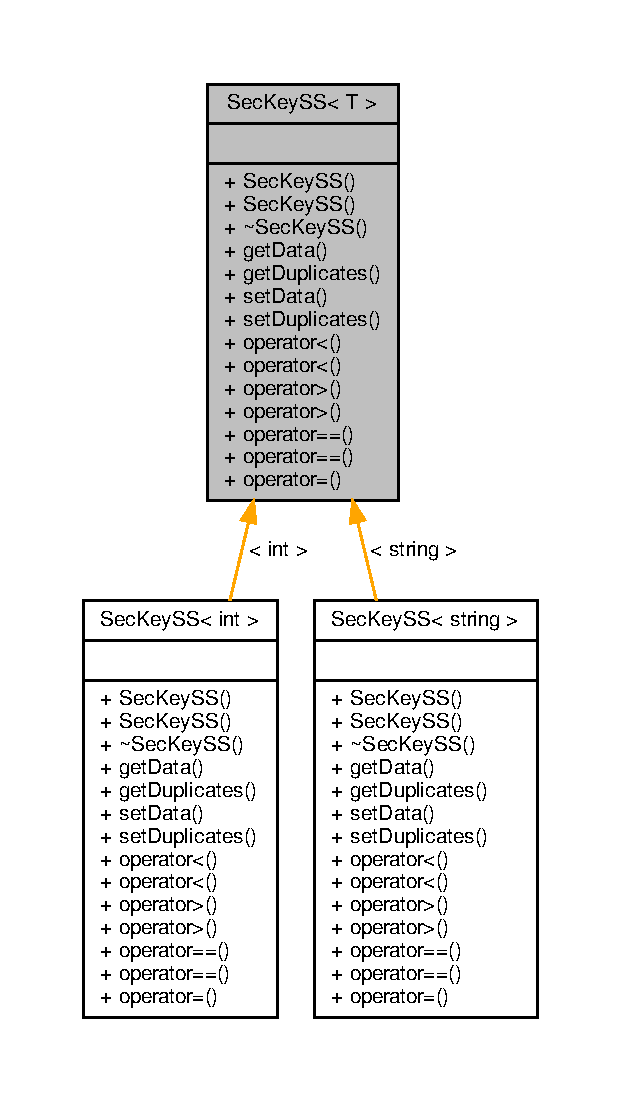
\includegraphics[width=298pt]{classSecKeySS__inherit__graph}
\end{center}
\end{figure}


Collaboration diagram for Sec\+Key\+SS$<$ T $>$\+:\nopagebreak
\begin{figure}[H]
\begin{center}
\leavevmode
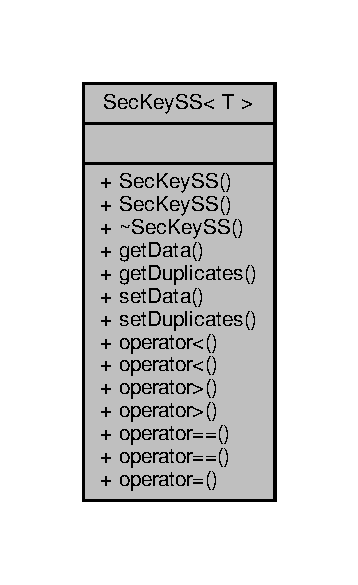
\includegraphics[width=172pt]{classSecKeySS__coll__graph}
\end{center}
\end{figure}
\subsection*{Public Member Functions}
\begin{DoxyCompactItemize}
\item 
\hyperlink{classSecKeySS_a9f905dffce0987d620cb2883b3f774cc}{Sec\+Key\+SS} ()
\item 
\hyperlink{classSecKeySS_ac9aecc7e01d33d17a98b732ac4f864c9}{Sec\+Key\+SS} (\hyperlink{classSecKeySS}{Sec\+Key\+SS}$<$ T $>$ \&s)
\item 
\hyperlink{classSecKeySS_ada9aac8a98536f84b46bc04b7acf9fec}{$\sim$\+Sec\+Key\+SS} ()
\item 
T \hyperlink{classSecKeySS_a9fdb8a771250b7aaab556f019b381eab}{get\+Data} () const
\item 
\hyperlink{classLinkedList}{Linked\+List}$<$ T $>$ \hyperlink{classSecKeySS_abef7c9c03e9bc6b818d599966428fdec}{get\+Duplicates} ()
\item 
void \hyperlink{classSecKeySS_ae893fbaf619bf61f73f1585ae5686609}{set\+Data} (const T s)
\item 
void \hyperlink{classSecKeySS_a95fdde8fc0b590359692784d15481dd4}{set\+Duplicates} (\hyperlink{classLinkedList}{Linked\+List}$<$ T $>$ dup)
\item 
bool \hyperlink{classSecKeySS_a4a77c5d5b609ef01c17f82001e9f1a7b}{operator$<$} (const T \&s) const
\item 
bool \hyperlink{classSecKeySS_ae39c46934a033ff213c1d1a7a32cd2bf}{operator$<$} (const \hyperlink{classSecKeySS}{Sec\+Key\+SS}$<$ T $>$ \&s) const
\item 
bool \hyperlink{classSecKeySS_a31bd2d2a2d8eeed14d478cbe88365843}{operator$>$} (const T \&s) const
\item 
bool \hyperlink{classSecKeySS_a5c5416d15e14212627b1076644abbb42}{operator$>$} (const \hyperlink{classSecKeySS}{Sec\+Key\+SS}$<$ T $>$ \&s) const
\item 
bool \hyperlink{classSecKeySS_ace15e2f5c729c58526f97919aff33036}{operator==} (const T \&s) const
\item 
bool \hyperlink{classSecKeySS_abf4a9212fdc1af29ddf44d5cbd6efca7}{operator==} (const \hyperlink{classSecKeySS}{Sec\+Key\+SS}$<$ T $>$ \&s) const
\item 
void \hyperlink{classSecKeySS_a2a04aabc21e56094354fd6c843d5a491}{operator=} (const \hyperlink{classSecKeySS}{Sec\+Key\+SS}$<$ T $>$ \&s)
\end{DoxyCompactItemize}


\subsection{Detailed Description}
\subsubsection*{template$<$typename T$>$\newline
class Sec\+Key\+S\+S$<$ T $>$}

This is the class for Section Keys of the SS class. 

\subsection{Constructor \& Destructor Documentation}
\mbox{\Hypertarget{classSecKeySS_a9f905dffce0987d620cb2883b3f774cc}\label{classSecKeySS_a9f905dffce0987d620cb2883b3f774cc}} 
\index{Sec\+Key\+SS@{Sec\+Key\+SS}!Sec\+Key\+SS@{Sec\+Key\+SS}}
\index{Sec\+Key\+SS@{Sec\+Key\+SS}!Sec\+Key\+SS@{Sec\+Key\+SS}}
\subsubsection{\texorpdfstring{Sec\+Key\+S\+S()}{SecKeySS()}\hspace{0.1cm}{\footnotesize\ttfamily [1/2]}}
{\footnotesize\ttfamily template$<$typename T$>$ \\
\hyperlink{classSecKeySS}{Sec\+Key\+SS}$<$ T $>$\+::\hyperlink{classSecKeySS}{Sec\+Key\+SS} (\begin{DoxyParamCaption}{ }\end{DoxyParamCaption})\hspace{0.3cm}{\ttfamily [inline]}}

Default constructor \mbox{\Hypertarget{classSecKeySS_ac9aecc7e01d33d17a98b732ac4f864c9}\label{classSecKeySS_ac9aecc7e01d33d17a98b732ac4f864c9}} 
\index{Sec\+Key\+SS@{Sec\+Key\+SS}!Sec\+Key\+SS@{Sec\+Key\+SS}}
\index{Sec\+Key\+SS@{Sec\+Key\+SS}!Sec\+Key\+SS@{Sec\+Key\+SS}}
\subsubsection{\texorpdfstring{Sec\+Key\+S\+S()}{SecKeySS()}\hspace{0.1cm}{\footnotesize\ttfamily [2/2]}}
{\footnotesize\ttfamily template$<$typename T$>$ \\
\hyperlink{classSecKeySS}{Sec\+Key\+SS}$<$ T $>$\+::\hyperlink{classSecKeySS}{Sec\+Key\+SS} (\begin{DoxyParamCaption}\item[{\hyperlink{classSecKeySS}{Sec\+Key\+SS}$<$ T $>$ \&}]{s }\end{DoxyParamCaption})}

Copy Constructor \mbox{\Hypertarget{classSecKeySS_ada9aac8a98536f84b46bc04b7acf9fec}\label{classSecKeySS_ada9aac8a98536f84b46bc04b7acf9fec}} 
\index{Sec\+Key\+SS@{Sec\+Key\+SS}!````~Sec\+Key\+SS@{$\sim$\+Sec\+Key\+SS}}
\index{````~Sec\+Key\+SS@{$\sim$\+Sec\+Key\+SS}!Sec\+Key\+SS@{Sec\+Key\+SS}}
\subsubsection{\texorpdfstring{$\sim$\+Sec\+Key\+S\+S()}{~SecKeySS()}}
{\footnotesize\ttfamily template$<$typename T $>$ \\
\hyperlink{classSecKeySS}{Sec\+Key\+SS}$<$ T $>$\+::$\sim$\hyperlink{classSecKeySS}{Sec\+Key\+SS} (\begin{DoxyParamCaption}{ }\end{DoxyParamCaption})}

Deconstuctor 

\subsection{Member Function Documentation}
\mbox{\Hypertarget{classSecKeySS_a9fdb8a771250b7aaab556f019b381eab}\label{classSecKeySS_a9fdb8a771250b7aaab556f019b381eab}} 
\index{Sec\+Key\+SS@{Sec\+Key\+SS}!get\+Data@{get\+Data}}
\index{get\+Data@{get\+Data}!Sec\+Key\+SS@{Sec\+Key\+SS}}
\subsubsection{\texorpdfstring{get\+Data()}{getData()}}
{\footnotesize\ttfamily template$<$typename T$>$ \\
T \hyperlink{classSecKeySS}{Sec\+Key\+SS}$<$ T $>$\+::get\+Data (\begin{DoxyParamCaption}{ }\end{DoxyParamCaption}) const\hspace{0.3cm}{\ttfamily [inline]}}

Gets data \begin{DoxyReturn}{Returns}
data the data to be returned 
\end{DoxyReturn}
\mbox{\Hypertarget{classSecKeySS_abef7c9c03e9bc6b818d599966428fdec}\label{classSecKeySS_abef7c9c03e9bc6b818d599966428fdec}} 
\index{Sec\+Key\+SS@{Sec\+Key\+SS}!get\+Duplicates@{get\+Duplicates}}
\index{get\+Duplicates@{get\+Duplicates}!Sec\+Key\+SS@{Sec\+Key\+SS}}
\subsubsection{\texorpdfstring{get\+Duplicates()}{getDuplicates()}}
{\footnotesize\ttfamily template$<$typename T $>$ \\
\hyperlink{classLinkedList}{Linked\+List}$<$ T $>$ \hyperlink{classSecKeySS}{Sec\+Key\+SS}$<$ T $>$\+::get\+Duplicates (\begin{DoxyParamCaption}{ }\end{DoxyParamCaption})}

Gets duplicates \begin{DoxyReturn}{Returns}
\hyperlink{classLinkedList}{Linked\+List} of item\+Type 
\end{DoxyReturn}
\mbox{\Hypertarget{classSecKeySS_a4a77c5d5b609ef01c17f82001e9f1a7b}\label{classSecKeySS_a4a77c5d5b609ef01c17f82001e9f1a7b}} 
\index{Sec\+Key\+SS@{Sec\+Key\+SS}!operator$<$@{operator$<$}}
\index{operator$<$@{operator$<$}!Sec\+Key\+SS@{Sec\+Key\+SS}}
\subsubsection{\texorpdfstring{operator$<$()}{operator<()}\hspace{0.1cm}{\footnotesize\ttfamily [1/2]}}
{\footnotesize\ttfamily template$<$typename T$>$ \\
bool \hyperlink{classSecKeySS}{Sec\+Key\+SS}$<$ T $>$\+::operator$<$ (\begin{DoxyParamCaption}\item[{const T \&}]{s }\end{DoxyParamCaption}) const\hspace{0.3cm}{\ttfamily [inline]}}

Operator less than 
\begin{DoxyParams}{Parameters}
{\em s} & a reference to a string to check if than \\
\hline
\end{DoxyParams}
\begin{DoxyReturn}{Returns}
true is data $<$ s 
\end{DoxyReturn}
\mbox{\Hypertarget{classSecKeySS_ae39c46934a033ff213c1d1a7a32cd2bf}\label{classSecKeySS_ae39c46934a033ff213c1d1a7a32cd2bf}} 
\index{Sec\+Key\+SS@{Sec\+Key\+SS}!operator$<$@{operator$<$}}
\index{operator$<$@{operator$<$}!Sec\+Key\+SS@{Sec\+Key\+SS}}
\subsubsection{\texorpdfstring{operator$<$()}{operator<()}\hspace{0.1cm}{\footnotesize\ttfamily [2/2]}}
{\footnotesize\ttfamily template$<$typename T$>$ \\
bool \hyperlink{classSecKeySS}{Sec\+Key\+SS}$<$ T $>$\+::operator$<$ (\begin{DoxyParamCaption}\item[{const \hyperlink{classSecKeySS}{Sec\+Key\+SS}$<$ T $>$ \&}]{s }\end{DoxyParamCaption}) const\hspace{0.3cm}{\ttfamily [inline]}}

Operator less than to check Sec key 
\begin{DoxyParams}{Parameters}
{\em s} & a string to check if than \\
\hline
\end{DoxyParams}
\begin{DoxyReturn}{Returns}
true is data $<$ s.\+data 
\end{DoxyReturn}
\mbox{\Hypertarget{classSecKeySS_a2a04aabc21e56094354fd6c843d5a491}\label{classSecKeySS_a2a04aabc21e56094354fd6c843d5a491}} 
\index{Sec\+Key\+SS@{Sec\+Key\+SS}!operator=@{operator=}}
\index{operator=@{operator=}!Sec\+Key\+SS@{Sec\+Key\+SS}}
\subsubsection{\texorpdfstring{operator=()}{operator=()}}
{\footnotesize\ttfamily template$<$typename T$>$ \\
void \hyperlink{classSecKeySS}{Sec\+Key\+SS}$<$ T $>$\+::operator= (\begin{DoxyParamCaption}\item[{const \hyperlink{classSecKeySS}{Sec\+Key\+SS}$<$ T $>$ \&}]{s }\end{DoxyParamCaption})}

Operator equal for copy constructor 
\begin{DoxyParams}{Parameters}
{\em s} & a reference to a \hyperlink{classSecKeySS}{Sec\+Key\+SS} \\
\hline
\end{DoxyParams}
\mbox{\Hypertarget{classSecKeySS_ace15e2f5c729c58526f97919aff33036}\label{classSecKeySS_ace15e2f5c729c58526f97919aff33036}} 
\index{Sec\+Key\+SS@{Sec\+Key\+SS}!operator==@{operator==}}
\index{operator==@{operator==}!Sec\+Key\+SS@{Sec\+Key\+SS}}
\subsubsection{\texorpdfstring{operator==()}{operator==()}\hspace{0.1cm}{\footnotesize\ttfamily [1/2]}}
{\footnotesize\ttfamily template$<$typename T$>$ \\
bool \hyperlink{classSecKeySS}{Sec\+Key\+SS}$<$ T $>$\+::operator== (\begin{DoxyParamCaption}\item[{const T \&}]{s }\end{DoxyParamCaption}) const\hspace{0.3cm}{\ttfamily [inline]}}

Operator is equal 
\begin{DoxyParams}{Parameters}
{\em s} & a reference to a string \\
\hline
\end{DoxyParams}
\begin{DoxyReturn}{Returns}
true if data is equal to s 
\end{DoxyReturn}
\mbox{\Hypertarget{classSecKeySS_abf4a9212fdc1af29ddf44d5cbd6efca7}\label{classSecKeySS_abf4a9212fdc1af29ddf44d5cbd6efca7}} 
\index{Sec\+Key\+SS@{Sec\+Key\+SS}!operator==@{operator==}}
\index{operator==@{operator==}!Sec\+Key\+SS@{Sec\+Key\+SS}}
\subsubsection{\texorpdfstring{operator==()}{operator==()}\hspace{0.1cm}{\footnotesize\ttfamily [2/2]}}
{\footnotesize\ttfamily template$<$typename T$>$ \\
bool \hyperlink{classSecKeySS}{Sec\+Key\+SS}$<$ T $>$\+::operator== (\begin{DoxyParamCaption}\item[{const \hyperlink{classSecKeySS}{Sec\+Key\+SS}$<$ T $>$ \&}]{s }\end{DoxyParamCaption}) const\hspace{0.3cm}{\ttfamily [inline]}}

Operator is equal 
\begin{DoxyParams}{Parameters}
{\em s} & a reference to a sec\+Key\+SS \\
\hline
\end{DoxyParams}
\begin{DoxyReturn}{Returns}
true if data is equal to s.\+data 
\end{DoxyReturn}
\mbox{\Hypertarget{classSecKeySS_a31bd2d2a2d8eeed14d478cbe88365843}\label{classSecKeySS_a31bd2d2a2d8eeed14d478cbe88365843}} 
\index{Sec\+Key\+SS@{Sec\+Key\+SS}!operator$>$@{operator$>$}}
\index{operator$>$@{operator$>$}!Sec\+Key\+SS@{Sec\+Key\+SS}}
\subsubsection{\texorpdfstring{operator$>$()}{operator>()}\hspace{0.1cm}{\footnotesize\ttfamily [1/2]}}
{\footnotesize\ttfamily template$<$typename T$>$ \\
bool \hyperlink{classSecKeySS}{Sec\+Key\+SS}$<$ T $>$\+::operator$>$ (\begin{DoxyParamCaption}\item[{const T \&}]{s }\end{DoxyParamCaption}) const\hspace{0.3cm}{\ttfamily [inline]}}

Operator geater than 
\begin{DoxyParams}{Parameters}
{\em s} & a reference to a string to check if $>$ than \\
\hline
\end{DoxyParams}
\begin{DoxyReturn}{Returns}
true is data $>$ s 
\end{DoxyReturn}
\mbox{\Hypertarget{classSecKeySS_a5c5416d15e14212627b1076644abbb42}\label{classSecKeySS_a5c5416d15e14212627b1076644abbb42}} 
\index{Sec\+Key\+SS@{Sec\+Key\+SS}!operator$>$@{operator$>$}}
\index{operator$>$@{operator$>$}!Sec\+Key\+SS@{Sec\+Key\+SS}}
\subsubsection{\texorpdfstring{operator$>$()}{operator>()}\hspace{0.1cm}{\footnotesize\ttfamily [2/2]}}
{\footnotesize\ttfamily template$<$typename T$>$ \\
bool \hyperlink{classSecKeySS}{Sec\+Key\+SS}$<$ T $>$\+::operator$>$ (\begin{DoxyParamCaption}\item[{const \hyperlink{classSecKeySS}{Sec\+Key\+SS}$<$ T $>$ \&}]{s }\end{DoxyParamCaption}) const\hspace{0.3cm}{\ttfamily [inline]}}

Operator greater than to check a Sec key 
\begin{DoxyParams}{Parameters}
{\em s} & a string to check if greater than \\
\hline
\end{DoxyParams}
\begin{DoxyReturn}{Returns}
true is data $>$ s.\+data 
\end{DoxyReturn}
\mbox{\Hypertarget{classSecKeySS_ae893fbaf619bf61f73f1585ae5686609}\label{classSecKeySS_ae893fbaf619bf61f73f1585ae5686609}} 
\index{Sec\+Key\+SS@{Sec\+Key\+SS}!set\+Data@{set\+Data}}
\index{set\+Data@{set\+Data}!Sec\+Key\+SS@{Sec\+Key\+SS}}
\subsubsection{\texorpdfstring{set\+Data()}{setData()}}
{\footnotesize\ttfamily template$<$typename T$>$ \\
void \hyperlink{classSecKeySS}{Sec\+Key\+SS}$<$ T $>$\+::set\+Data (\begin{DoxyParamCaption}\item[{const T}]{s }\end{DoxyParamCaption})\hspace{0.3cm}{\ttfamily [inline]}}

Sets the data equal to argument 1 
\begin{DoxyParams}{Parameters}
{\em s} & a string to set data to \\
\hline
\end{DoxyParams}
\mbox{\Hypertarget{classSecKeySS_a95fdde8fc0b590359692784d15481dd4}\label{classSecKeySS_a95fdde8fc0b590359692784d15481dd4}} 
\index{Sec\+Key\+SS@{Sec\+Key\+SS}!set\+Duplicates@{set\+Duplicates}}
\index{set\+Duplicates@{set\+Duplicates}!Sec\+Key\+SS@{Sec\+Key\+SS}}
\subsubsection{\texorpdfstring{set\+Duplicates()}{setDuplicates()}}
{\footnotesize\ttfamily template$<$typename T$>$ \\
void \hyperlink{classSecKeySS}{Sec\+Key\+SS}$<$ T $>$\+::set\+Duplicates (\begin{DoxyParamCaption}\item[{\hyperlink{classLinkedList}{Linked\+List}$<$ T $>$}]{dup }\end{DoxyParamCaption})}

Sets duplicates 
\begin{DoxyParams}{Parameters}
{\em \hyperlink{classLinkedList}{Linked\+List}} & dup \\
\hline
\end{DoxyParams}


The documentation for this class was generated from the following file\+:\begin{DoxyCompactItemize}
\item 
\hyperlink{SecKeySS_8h}{Sec\+Key\+S\+S.\+h}\end{DoxyCompactItemize}

\hypertarget{classSSClass}{}\section{S\+S\+Class Class Reference}
\label{classSSClass}\index{S\+S\+Class@{S\+S\+Class}}


\hyperlink{classLinkedList}{Linked\+List} integration for blocks, records, and fields.  




{\ttfamily \#include \char`\"{}S\+S\+Class.\+h\char`\"{}}

\subsection*{Public Member Functions}
\begin{DoxyCompactItemize}
\item 
\mbox{\Hypertarget{classSSClass_ab4603d6a236c4fa65f896a1158c0d2ef}\label{classSSClass_ab4603d6a236c4fa65f896a1158c0d2ef}} 
\hyperlink{classSSClass_ab4603d6a236c4fa65f896a1158c0d2ef}{S\+S\+Class} ()
\begin{DoxyCompactList}\small\item\em Default constructor. \end{DoxyCompactList}\item 
\mbox{\Hypertarget{classSSClass_a5801614847b5403b1a5899150acd3b5c}\label{classSSClass_a5801614847b5403b1a5899150acd3b5c}} 
\hyperlink{classSSClass_a5801614847b5403b1a5899150acd3b5c}{S\+S\+Class} (const \hyperlink{classSSClass}{S\+S\+Class} \&ss)
\begin{DoxyCompactList}\small\item\em Constructor. \end{DoxyCompactList}\item 
\mbox{\Hypertarget{classSSClass_a6e5abb04de9b90e34cc6422069ff5729}\label{classSSClass_a6e5abb04de9b90e34cc6422069ff5729}} 
\hyperlink{classSSClass_a6e5abb04de9b90e34cc6422069ff5729}{$\sim$\+S\+S\+Class} ()
\begin{DoxyCompactList}\small\item\em Deconstructor. \end{DoxyCompactList}\item 
bool \hyperlink{classSSClass_afc95611385e4d389818332414d5c491c}{is\+Empty} ()
\begin{DoxyCompactList}\small\item\em Check if num\+Records is 0. \end{DoxyCompactList}\item 
bool \hyperlink{classSSClass_a92e012441608ea36f3013fb3cbea9da8}{open\+File} (string input)
\begin{DoxyCompactList}\small\item\em Opens external file. \end{DoxyCompactList}\item 
void \hyperlink{classSSClass_a45c5585c784bf7c4f823f66426664aea}{insert} (string s)
\begin{DoxyCompactList}\small\item\em inserts line by line into data \end{DoxyCompactList}\item 
vector$<$ int $>$ \hyperlink{classSSClass_a9df3598c000a6a5e9ef994d19196e69f}{search} (string s, unsigned field\+Num)
\begin{DoxyCompactList}\small\item\em Searches for record. \end{DoxyCompactList}\item 
int \hyperlink{classSSClass_ad03c99840c2946a2112f5f1942c287f2}{directional\+Search} (string state, char direction)
\begin{DoxyCompactList}\small\item\em Searches directionly (N, S, W, E) \end{DoxyCompactList}\item 
string \hyperlink{classSSClass_ab0a8ea1af895df28359b5733bd920ef3}{return\+Line} (int rrn)
\begin{DoxyCompactList}\small\item\em Fills secondary key vector. \end{DoxyCompactList}\end{DoxyCompactItemize}


\subsection{Detailed Description}
\hyperlink{classLinkedList}{Linked\+List} integration for blocks, records, and fields. 

\begin{DoxyAuthor}{Authors}
Jordan Bremer, Melvin Schmid, ..., ..., ...
\end{DoxyAuthor}
Sequence Set class\+: -- allows for insert and deletion of linked list -- populates secondary keys -- allows for searching of said linked list -- ability to return city, state, county, lattitude, longitude, zip, and lower and upper indicies -- ability to input a txt file and populate it\textquotesingle{}s contents

Implementation and assumptions\+: -- size defaults are listed towards the top of the program -- array/vector elements are initialized to zero 

Definition at line 65 of file S\+S\+Class.\+h.



\subsection{Member Function Documentation}
\mbox{\Hypertarget{classSSClass_ad03c99840c2946a2112f5f1942c287f2}\label{classSSClass_ad03c99840c2946a2112f5f1942c287f2}} 
\index{S\+S\+Class@{S\+S\+Class}!directional\+Search@{directional\+Search}}
\index{directional\+Search@{directional\+Search}!S\+S\+Class@{S\+S\+Class}}
\subsubsection{\texorpdfstring{directional\+Search()}{directionalSearch()}}
{\footnotesize\ttfamily int S\+S\+Class\+::directional\+Search (\begin{DoxyParamCaption}\item[{string}]{state,  }\item[{char}]{direction }\end{DoxyParamCaption})}



Searches directionly (N, S, W, E) 


\begin{DoxyParams}{Parameters}
{\em state} & the state to search \\
\hline
{\em direction} & (N, S, W, E) \\
\hline
\end{DoxyParams}
\begin{DoxyReturn}{Returns}
the line contating the soght after direction 
\end{DoxyReturn}


Definition at line 431 of file S\+S\+Class.\+h.


\begin{DoxyCode}
431                                                             \{
432     direction = toupper(direction);
433     \textcolor{keywordtype}{int} i = 1;
434     \textcolor{keywordtype}{int} returnIndex = -1;
435     \textcolor{keywordtype}{double} highOrLow;
436     vector<int> state = \hyperlink{classSSClass_a9df3598c000a6a5e9ef994d19196e69f}{search}(stateS, 3);
437     \textcolor{keywordflow}{switch} (direction) \{
438     \textcolor{keywordflow}{case} \textcolor{charliteral}{'N'}:
439     \{
440         returnIndex = state[0];
441         highOrLow = stod(getLat(\hyperlink{classSSClass_ab0a8ea1af895df28359b5733bd920ef3}{returnLine}(state[0])));
442         \textcolor{keywordflow}{for} (i; i < state.size(); i++) \{
443             \textcolor{keywordflow}{if} (highOrLow < stod(getLat(\hyperlink{classSSClass_ab0a8ea1af895df28359b5733bd920ef3}{returnLine}(state[i])))) \{
444                 highOrLow = stod(getLat(\hyperlink{classSSClass_ab0a8ea1af895df28359b5733bd920ef3}{returnLine}(state[i])));
445                 returnIndex = i;
446             \}
447 
448         \}
449     \}
450     \textcolor{keywordflow}{break};
451     \textcolor{keywordflow}{case} \textcolor{charliteral}{'E'}:
452     \{
453         returnIndex = state[0];
454         highOrLow = stod(getLon(\hyperlink{classSSClass_ab0a8ea1af895df28359b5733bd920ef3}{returnLine}(state[0])));
455         \textcolor{keywordflow}{for} (i; i < state.size(); i++) \{
456             \textcolor{keywordflow}{if} (highOrLow < stod(getLon(\hyperlink{classSSClass_ab0a8ea1af895df28359b5733bd920ef3}{returnLine}(state[i])))) \{
457                 highOrLow = stod(getLon(\hyperlink{classSSClass_ab0a8ea1af895df28359b5733bd920ef3}{returnLine}(state[i])));
458                 returnIndex = i;
459             \}
460         \}
461         
462     \}
463     \textcolor{keywordflow}{break};
464     \textcolor{keywordflow}{case} \textcolor{charliteral}{'S'}:
465     \{
466         returnIndex = state[0];
467         highOrLow = stod(getLat(\hyperlink{classSSClass_ab0a8ea1af895df28359b5733bd920ef3}{returnLine}(state[0])));
468         \textcolor{keywordflow}{for} (i; i < state.size(); i++) \{
469             \textcolor{keywordflow}{if} (highOrLow > stod(getLat(\hyperlink{classSSClass_ab0a8ea1af895df28359b5733bd920ef3}{returnLine}(state[i])))) \{
470                 highOrLow = stod(getLat(\hyperlink{classSSClass_ab0a8ea1af895df28359b5733bd920ef3}{returnLine}(state[i])));
471                 returnIndex = i;
472             \}
473         \}
474         \textcolor{keywordflow}{break};
475     \}
476     \textcolor{keywordflow}{case} \textcolor{charliteral}{'W'}:
477     \{
478         returnIndex = state[0];
479         highOrLow = stod(getLon(\hyperlink{classSSClass_ab0a8ea1af895df28359b5733bd920ef3}{returnLine}(state[0])));
480         \textcolor{keywordflow}{for} (i; i < state.size(); i++) \{
481             \textcolor{keywordflow}{if} (highOrLow > stod(getLon(\hyperlink{classSSClass_ab0a8ea1af895df28359b5733bd920ef3}{returnLine}(state[i])))) \{
482                 highOrLow = stod(getLon(\hyperlink{classSSClass_ab0a8ea1af895df28359b5733bd920ef3}{returnLine}(state[i])));
483                 returnIndex = i;
484             \}
485         \}
486 
487     \}
488     \textcolor{keywordflow}{break};
489     \}
490     \textcolor{keywordflow}{return} returnIndex;
491 
492 \}
\end{DoxyCode}
\mbox{\Hypertarget{classSSClass_a45c5585c784bf7c4f823f66426664aea}\label{classSSClass_a45c5585c784bf7c4f823f66426664aea}} 
\index{S\+S\+Class@{S\+S\+Class}!insert@{insert}}
\index{insert@{insert}!S\+S\+Class@{S\+S\+Class}}
\subsubsection{\texorpdfstring{insert()}{insert()}}
{\footnotesize\ttfamily void S\+S\+Class\+::insert (\begin{DoxyParamCaption}\item[{string}]{s }\end{DoxyParamCaption})}



inserts line by line into data 


\begin{DoxyParams}{Parameters}
{\em s} & a string to insert\\
\hline
\end{DoxyParams}
Insertion of records into both the index file as well as the linkedlist of linkedlists /param s string to be inserted 

Definition at line 325 of file S\+S\+Class.\+h.


\begin{DoxyCode}
325                              \{
326     \textcolor{keywordflow}{if} (nextEmpty == -1) \{
327         goToLine(indexFile, numLinesIndex);
328         indexFile << \textcolor{stringliteral}{"\(\backslash\)n"} << s;
329         insertZip(getZip(s), numLinesIndex);
330         insertPlace(getPlace(s), numLinesIndex);
331         insertState(getState(s), numLinesIndex);
332         insertCounty(getCounty(s), numLinesIndex);
333         insertLat(getLat(s), numLinesIndex);
334         insertLon(getLon(s), numLinesIndex);
335         numLinesIndex++;
336         \textcolor{keywordflow}{return};
337     \}
338     goToLine(indexFile, nextEmpty);
339     \textcolor{comment}{//replace(s, nextEmpty);}
340     insertZip(getZip(s), nextEmpty);
341     insertPlace(getPlace(s), nextEmpty);
342     insertState(getState(s), nextEmpty);
343     insertCounty(getCounty(s), nextEmpty);
344     insertLat(getLat(s), nextEmpty);
345     insertLon(getLon(s), nextEmpty);
346 \}
\end{DoxyCode}
\mbox{\Hypertarget{classSSClass_afc95611385e4d389818332414d5c491c}\label{classSSClass_afc95611385e4d389818332414d5c491c}} 
\index{S\+S\+Class@{S\+S\+Class}!is\+Empty@{is\+Empty}}
\index{is\+Empty@{is\+Empty}!S\+S\+Class@{S\+S\+Class}}
\subsubsection{\texorpdfstring{is\+Empty()}{isEmpty()}}
{\footnotesize\ttfamily bool S\+S\+Class\+::is\+Empty (\begin{DoxyParamCaption}{ }\end{DoxyParamCaption})\hspace{0.3cm}{\ttfamily [inline]}}



Check if num\+Records is 0. 

\begin{DoxyReturn}{Returns}
returns false if empty, otherwise returns true 
\end{DoxyReturn}


Definition at line 206 of file S\+S\+Class.\+h.


\begin{DoxyCode}
206 \{ \textcolor{keywordflow}{return} numRecords == 0; \};
\end{DoxyCode}
\mbox{\Hypertarget{classSSClass_a92e012441608ea36f3013fb3cbea9da8}\label{classSSClass_a92e012441608ea36f3013fb3cbea9da8}} 
\index{S\+S\+Class@{S\+S\+Class}!open\+File@{open\+File}}
\index{open\+File@{open\+File}!S\+S\+Class@{S\+S\+Class}}
\subsubsection{\texorpdfstring{open\+File()}{openFile()}}
{\footnotesize\ttfamily bool S\+S\+Class\+::open\+File (\begin{DoxyParamCaption}\item[{string}]{input }\end{DoxyParamCaption})}



Opens external file. 


\begin{DoxyParams}{Parameters}
{\em input} & string \\
\hline
\end{DoxyParams}
\begin{DoxyPrecond}{Precondition}
data file 
\end{DoxyPrecond}
\begin{DoxyReturn}{Returns}
true if file location exists, otherwise returns false 
\end{DoxyReturn}


Definition at line 261 of file S\+S\+Class.\+h.


\begin{DoxyCode}
261                                    \{ \textcolor{comment}{//input is a file name}
262     indexFile.open(input);
263     nextEmpty = -1;
264     \textcolor{keywordflow}{return} (indexFile.is\_open());
265 
266 \}
\end{DoxyCode}
\mbox{\Hypertarget{classSSClass_ab0a8ea1af895df28359b5733bd920ef3}\label{classSSClass_ab0a8ea1af895df28359b5733bd920ef3}} 
\index{S\+S\+Class@{S\+S\+Class}!return\+Line@{return\+Line}}
\index{return\+Line@{return\+Line}!S\+S\+Class@{S\+S\+Class}}
\subsubsection{\texorpdfstring{return\+Line()}{returnLine()}}
{\footnotesize\ttfamily string S\+S\+Class\+::return\+Line (\begin{DoxyParamCaption}\item[{int}]{rrn }\end{DoxyParamCaption})}



Fills secondary key vector. 


\begin{DoxyParams}{Parameters}
{\em rrn} & and integer refring to the line to get \\
\hline
\end{DoxyParams}
\begin{DoxyReturn}{Returns}
string containging the contents of the line 
\end{DoxyReturn}


Definition at line 348 of file S\+S\+Class.\+h.


\begin{DoxyCode}
348                                   \{
349     \textcolor{keywordtype}{string} returnVal;
350     goToLine(indexFile, rrn);
351     getline(indexFile, returnVal);
352     \textcolor{keywordflow}{return} returnVal;
353 \}
\end{DoxyCode}
\mbox{\Hypertarget{classSSClass_a9df3598c000a6a5e9ef994d19196e69f}\label{classSSClass_a9df3598c000a6a5e9ef994d19196e69f}} 
\index{S\+S\+Class@{S\+S\+Class}!search@{search}}
\index{search@{search}!S\+S\+Class@{S\+S\+Class}}
\subsubsection{\texorpdfstring{search()}{search()}}
{\footnotesize\ttfamily vector$<$ int $>$ S\+S\+Class\+::search (\begin{DoxyParamCaption}\item[{string}]{s,  }\item[{unsigned}]{field\+Num }\end{DoxyParamCaption})}



Searches for record. 


\begin{DoxyParams}{Parameters}
{\em s} & strign to search for  field\+Num the field in whitch to search \\
\hline
\end{DoxyParams}
\begin{DoxyReturn}{Returns}
vector of results 
\end{DoxyReturn}


Definition at line 356 of file S\+S\+Class.\+h.


\begin{DoxyCode}
356                                                        \{
357     \hyperlink{classSecKeySS}{SecKeySS} secCopy;
358     \textcolor{keywordtype}{int} i;
359     vector<int> results;
360     \textcolor{keywordflow}{switch} (fieldNum) \{
361     \textcolor{keywordflow}{case} 1:
362     \{
363         \textcolor{keywordflow}{for} (i = 1; (i < (secKeyZip.\hyperlink{classLinkedList_afc6635f854f48f2f126cf3b60d845220}{getItemCount}() + 1)) && (secKeyZip.
      \hyperlink{classLinkedList_a341bfd7772c9d24d29eb7a7f3936915b}{getEntry}(i).\hyperlink{classSecKeySS_add52510d280d0ca89b653386500f08f5}{getData}() < s); i++);
364         \textcolor{keywordflow}{if} (stoi(secKeyZip.\hyperlink{classLinkedList_a341bfd7772c9d24d29eb7a7f3936915b}{getEntry}(i).\hyperlink{classSecKeySS_add52510d280d0ca89b653386500f08f5}{getData}()) == stoi(s)) \{
365             \hyperlink{classLinkedList}{LinkedList<int>} toCopy = \hyperlink{classLinkedList}{LinkedList<int>}(secKeyZip.
      \hyperlink{classLinkedList_a341bfd7772c9d24d29eb7a7f3936915b}{getEntry}(i).\hyperlink{classSecKeySS_aaae9db891cfcdc3f78d8a44145f4f08c}{getDuplicates}());
366             \textcolor{keywordflow}{for} (\textcolor{keywordtype}{int} j = 1; j < (toCopy.\hyperlink{classLinkedList_afc6635f854f48f2f126cf3b60d845220}{getItemCount}() + 1); j++) \{
367                 results.push\_back(toCopy.\hyperlink{classLinkedList_a341bfd7772c9d24d29eb7a7f3936915b}{getEntry}(j));
368             \}
369         \}
370     \}
371     \textcolor{keywordflow}{break};
372     \textcolor{keywordflow}{case} 2:
373     \{
374         \textcolor{keywordflow}{for}(i = 1; (i < (secKeyPlace.\hyperlink{classLinkedList_afc6635f854f48f2f126cf3b60d845220}{getItemCount}() + 1)) && (secKeyPlace.
      \hyperlink{classLinkedList_a341bfd7772c9d24d29eb7a7f3936915b}{getEntry}(i).\hyperlink{classSecKeySS_add52510d280d0ca89b653386500f08f5}{getData}() < s); i++);
375         \textcolor{keywordflow}{if} ((secKeyPlace.\hyperlink{classLinkedList_a341bfd7772c9d24d29eb7a7f3936915b}{getEntry}(i).\hyperlink{classSecKeySS_add52510d280d0ca89b653386500f08f5}{getData}()) == (s)) \{
376             \hyperlink{classLinkedList}{LinkedList<int>} toCopy = \hyperlink{classLinkedList}{LinkedList<int>}(secKeyPlace.
      \hyperlink{classLinkedList_a341bfd7772c9d24d29eb7a7f3936915b}{getEntry}(i).\hyperlink{classSecKeySS_aaae9db891cfcdc3f78d8a44145f4f08c}{getDuplicates}());
377             \textcolor{keywordflow}{for} (\textcolor{keywordtype}{int} j = 1; j < (toCopy.\hyperlink{classLinkedList_afc6635f854f48f2f126cf3b60d845220}{getItemCount}() + 1); j++) \{
378                 results.push\_back(toCopy.\hyperlink{classLinkedList_a341bfd7772c9d24d29eb7a7f3936915b}{getEntry}(j));
379             \}
380         \}
381     \}
382     \textcolor{keywordflow}{break};
383     \textcolor{keywordflow}{case} 3:
384     \{
385         \textcolor{keywordflow}{for} (i = 1; (i < (secKeyState.\hyperlink{classLinkedList_afc6635f854f48f2f126cf3b60d845220}{getItemCount}() + 1)) && (secKeyState.
      \hyperlink{classLinkedList_a341bfd7772c9d24d29eb7a7f3936915b}{getEntry}(i).\hyperlink{classSecKeySS_add52510d280d0ca89b653386500f08f5}{getData}() < s); i++);
386         \textcolor{keywordflow}{if} ((secKeyState.\hyperlink{classLinkedList_a341bfd7772c9d24d29eb7a7f3936915b}{getEntry}(i).\hyperlink{classSecKeySS_add52510d280d0ca89b653386500f08f5}{getData}()) == (s)) \{
387             \hyperlink{classLinkedList}{LinkedList<int>} toCopy = \hyperlink{classLinkedList}{LinkedList<int>}(secKeyState.
      \hyperlink{classLinkedList_a341bfd7772c9d24d29eb7a7f3936915b}{getEntry}(i).\hyperlink{classSecKeySS_aaae9db891cfcdc3f78d8a44145f4f08c}{getDuplicates}());
388             \textcolor{keywordflow}{for} (\textcolor{keywordtype}{int} j = 1; j < (toCopy.\hyperlink{classLinkedList_afc6635f854f48f2f126cf3b60d845220}{getItemCount}() + 1); j++) \{
389                 results.push\_back(toCopy.\hyperlink{classLinkedList_a341bfd7772c9d24d29eb7a7f3936915b}{getEntry}(j));
390             \}
391         \}
392     \}
393     \textcolor{keywordflow}{break};
394     \textcolor{keywordflow}{case} 4:
395     \{
396         \textcolor{keywordflow}{for} (i = 1; (i < (secKeyCounty.\hyperlink{classLinkedList_afc6635f854f48f2f126cf3b60d845220}{getItemCount}() + 1)) && (secKeyCounty.
      \hyperlink{classLinkedList_a341bfd7772c9d24d29eb7a7f3936915b}{getEntry}(i).\hyperlink{classSecKeySS_add52510d280d0ca89b653386500f08f5}{getData}() < s); i++);
397         \textcolor{keywordflow}{if} ((secKeyCounty.\hyperlink{classLinkedList_a341bfd7772c9d24d29eb7a7f3936915b}{getEntry}(i).\hyperlink{classSecKeySS_add52510d280d0ca89b653386500f08f5}{getData}()) == (s)) \{
398             \hyperlink{classLinkedList}{LinkedList<int>} toCopy = \hyperlink{classLinkedList}{LinkedList<int>}(secKeyCounty.
      \hyperlink{classLinkedList_a341bfd7772c9d24d29eb7a7f3936915b}{getEntry}(i).\hyperlink{classSecKeySS_aaae9db891cfcdc3f78d8a44145f4f08c}{getDuplicates}());
399             \textcolor{keywordflow}{for} (\textcolor{keywordtype}{int} j = 1; j < (toCopy.\hyperlink{classLinkedList_afc6635f854f48f2f126cf3b60d845220}{getItemCount}() + 1); j++) \{
400                 results.push\_back(toCopy.\hyperlink{classLinkedList_a341bfd7772c9d24d29eb7a7f3936915b}{getEntry}(j));
401             \}
402         \}
403     \}
404     \textcolor{keywordflow}{break};
405     \textcolor{keywordflow}{case} 5:
406     \{
407         \textcolor{keywordflow}{for} (i = 1; (i < (secKeyLat.\hyperlink{classLinkedList_afc6635f854f48f2f126cf3b60d845220}{getItemCount}() + 1)) && (secKeyLat.
      \hyperlink{classLinkedList_a341bfd7772c9d24d29eb7a7f3936915b}{getEntry}(i).\hyperlink{classSecKeySS_add52510d280d0ca89b653386500f08f5}{getData}() < s); i++);
408         \textcolor{keywordflow}{if} (stoi(secKeyLat.\hyperlink{classLinkedList_a341bfd7772c9d24d29eb7a7f3936915b}{getEntry}(i).\hyperlink{classSecKeySS_add52510d280d0ca89b653386500f08f5}{getData}()) == static\_cast<int>(stod(s))) \{
409             \hyperlink{classLinkedList}{LinkedList<int>} toCopy = \hyperlink{classLinkedList}{LinkedList<int>}(secKeyLat.
      \hyperlink{classLinkedList_a341bfd7772c9d24d29eb7a7f3936915b}{getEntry}(i).\hyperlink{classSecKeySS_aaae9db891cfcdc3f78d8a44145f4f08c}{getDuplicates}());
410             \textcolor{keywordflow}{for} (\textcolor{keywordtype}{int} j = 1; j < (toCopy.\hyperlink{classLinkedList_afc6635f854f48f2f126cf3b60d845220}{getItemCount}() + 1); j++) \{
411                 results.push\_back(toCopy.\hyperlink{classLinkedList_a341bfd7772c9d24d29eb7a7f3936915b}{getEntry}(j));
412             \}
413         \}
414     \}
415     \textcolor{keywordflow}{break};
416     \textcolor{keywordflow}{case} 6:
417     \{
418         \textcolor{keywordflow}{for} (i = 1; (i < (secKeyLon.\hyperlink{classLinkedList_afc6635f854f48f2f126cf3b60d845220}{getItemCount}() + 1)) && (secKeyLon.
      \hyperlink{classLinkedList_a341bfd7772c9d24d29eb7a7f3936915b}{getEntry}(i).\hyperlink{classSecKeySS_add52510d280d0ca89b653386500f08f5}{getData}() < s); i++);
419         \textcolor{keywordflow}{if} (stoi(secKeyLon.\hyperlink{classLinkedList_a341bfd7772c9d24d29eb7a7f3936915b}{getEntry}(i).\hyperlink{classSecKeySS_add52510d280d0ca89b653386500f08f5}{getData}()) == static\_cast<int>(stod(s))) \{
420             \hyperlink{classLinkedList}{LinkedList<int>} toCopy = \hyperlink{classLinkedList}{LinkedList<int>}(secKeyLon.
      \hyperlink{classLinkedList_a341bfd7772c9d24d29eb7a7f3936915b}{getEntry}(i).\hyperlink{classSecKeySS_aaae9db891cfcdc3f78d8a44145f4f08c}{getDuplicates}());
421             \textcolor{keywordflow}{for} (\textcolor{keywordtype}{int} j = 1; j < (toCopy.\hyperlink{classLinkedList_afc6635f854f48f2f126cf3b60d845220}{getItemCount}() + 1); j++) \{
422                 results.push\_back(toCopy.\hyperlink{classLinkedList_a341bfd7772c9d24d29eb7a7f3936915b}{getEntry}(j));
423             \}
424         \}
425     \}
426     \textcolor{keywordflow}{break};
427     \}
428     \textcolor{keywordflow}{return} results;
429 \}
\end{DoxyCode}


The documentation for this class was generated from the following file\+:\begin{DoxyCompactItemize}
\item 
S\+S\+Class.\+h\end{DoxyCompactItemize}

\chapter{File Documentation}
\hypertarget{BTree_8h}{}\section{B\+Tree.\+h File Reference}
\label{BTree_8h}\index{B\+Tree.\+h@{B\+Tree.\+h}}
{\ttfamily \#include $<$stdio.\+h$>$}\newline
{\ttfamily \#include $<$conio.\+h$>$}\newline
{\ttfamily \#include $<$iostream$>$}\newline
Include dependency graph for B\+Tree.\+h\+:\nopagebreak
\begin{figure}[H]
\begin{center}
\leavevmode
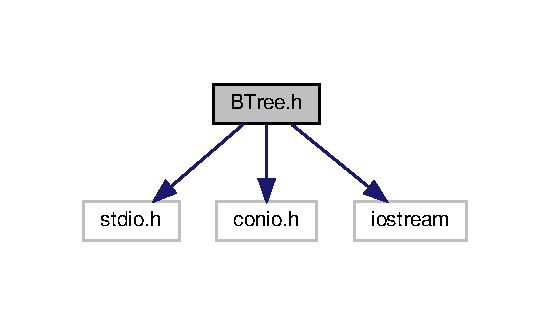
\includegraphics[width=264pt]{BTree_8h__incl}
\end{center}
\end{figure}
\subsection*{Classes}
\begin{DoxyCompactItemize}
\item 
struct \hyperlink{structBTreeNode}{B\+Tree\+Node$<$ T $>$}
\end{DoxyCompactItemize}
\subsection*{Functions}
\begin{DoxyCompactItemize}
\item 
{\footnotesize template$<$typename T $>$ }\\\hyperlink{structBTreeNode}{B\+Tree\+Node} $\ast$ \hyperlink{BTree_8h_a30a93849f7d32829662c20400ced546b}{init} ()
\item 
{\footnotesize template$<$typename T $>$ }\\void \hyperlink{BTree_8h_aeb0846dea9d7c76703072a63fdf91646}{traverse} (\hyperlink{structBTreeNode}{B\+Tree\+Node} $\ast$p)
\item 
{\footnotesize template$<$typename T $>$ }\\void \hyperlink{BTree_8h_aff368fafc4ab510f2054a0b8dd6ee685}{sort} (int $\ast$p, int n)
\item 
{\footnotesize template$<$typename T $>$ }\\T \hyperlink{BTree_8h_a80292238f91964bc30573f633a3b991c}{split\+\_\+child} (\hyperlink{structBTreeNode}{B\+Tree\+Node} $\ast$\hyperlink{BTree_8h_abd38bc6ba9fbde6b140bd94db822df78}{x}, int i)
\item 
{\footnotesize template$<$typename T $>$ }\\void \hyperlink{BTree_8h_ac86ce26a0b0ec9d79b918b285fe9da38}{insert} (T a)
\end{DoxyCompactItemize}
\subsection*{Variables}
\begin{DoxyCompactItemize}
\item 
struct \hyperlink{structBTreeNode}{B\+Tree\+Node} $\ast$ \hyperlink{BTree_8h_a060c65791205560994f49f7b4cdcd2f5}{root} = N\+U\+LL
\item 
struct \hyperlink{structBTreeNode}{B\+Tree\+Node} $\ast$ \hyperlink{BTree_8h_a84eeac28397095456715e78262e4fc9c}{np} = N\+U\+LL
\item 
struct \hyperlink{structBTreeNode}{B\+Tree\+Node} $\ast$ \hyperlink{BTree_8h_abd38bc6ba9fbde6b140bd94db822df78}{x} = N\+U\+LL
\end{DoxyCompactItemize}


\subsection{Function Documentation}
\mbox{\Hypertarget{BTree_8h_a30a93849f7d32829662c20400ced546b}\label{BTree_8h_a30a93849f7d32829662c20400ced546b}} 
\index{B\+Tree.\+h@{B\+Tree.\+h}!init@{init}}
\index{init@{init}!B\+Tree.\+h@{B\+Tree.\+h}}
\subsubsection{\texorpdfstring{init()}{init()}}
{\footnotesize\ttfamily template$<$typename T $>$ \\
\hyperlink{structBTreeNode}{B\+Tree\+Node}$\ast$ init (\begin{DoxyParamCaption}{ }\end{DoxyParamCaption})}

\mbox{\Hypertarget{BTree_8h_ac86ce26a0b0ec9d79b918b285fe9da38}\label{BTree_8h_ac86ce26a0b0ec9d79b918b285fe9da38}} 
\index{B\+Tree.\+h@{B\+Tree.\+h}!insert@{insert}}
\index{insert@{insert}!B\+Tree.\+h@{B\+Tree.\+h}}
\subsubsection{\texorpdfstring{insert()}{insert()}}
{\footnotesize\ttfamily template$<$typename T $>$ \\
void insert (\begin{DoxyParamCaption}\item[{T}]{a }\end{DoxyParamCaption})}

\mbox{\Hypertarget{BTree_8h_aff368fafc4ab510f2054a0b8dd6ee685}\label{BTree_8h_aff368fafc4ab510f2054a0b8dd6ee685}} 
\index{B\+Tree.\+h@{B\+Tree.\+h}!sort@{sort}}
\index{sort@{sort}!B\+Tree.\+h@{B\+Tree.\+h}}
\subsubsection{\texorpdfstring{sort()}{sort()}}
{\footnotesize\ttfamily template$<$typename T $>$ \\
void sort (\begin{DoxyParamCaption}\item[{int $\ast$}]{p,  }\item[{int}]{n }\end{DoxyParamCaption})}

\mbox{\Hypertarget{BTree_8h_a80292238f91964bc30573f633a3b991c}\label{BTree_8h_a80292238f91964bc30573f633a3b991c}} 
\index{B\+Tree.\+h@{B\+Tree.\+h}!split\+\_\+child@{split\+\_\+child}}
\index{split\+\_\+child@{split\+\_\+child}!B\+Tree.\+h@{B\+Tree.\+h}}
\subsubsection{\texorpdfstring{split\+\_\+child()}{split\_child()}}
{\footnotesize\ttfamily template$<$typename T $>$ \\
T split\+\_\+child (\begin{DoxyParamCaption}\item[{\hyperlink{structBTreeNode}{B\+Tree\+Node} $\ast$}]{x,  }\item[{int}]{i }\end{DoxyParamCaption})}

\mbox{\Hypertarget{BTree_8h_aeb0846dea9d7c76703072a63fdf91646}\label{BTree_8h_aeb0846dea9d7c76703072a63fdf91646}} 
\index{B\+Tree.\+h@{B\+Tree.\+h}!traverse@{traverse}}
\index{traverse@{traverse}!B\+Tree.\+h@{B\+Tree.\+h}}
\subsubsection{\texorpdfstring{traverse()}{traverse()}}
{\footnotesize\ttfamily template$<$typename T $>$ \\
void traverse (\begin{DoxyParamCaption}\item[{\hyperlink{structBTreeNode}{B\+Tree\+Node} $\ast$}]{p }\end{DoxyParamCaption})}



\subsection{Variable Documentation}
\mbox{\Hypertarget{BTree_8h_a84eeac28397095456715e78262e4fc9c}\label{BTree_8h_a84eeac28397095456715e78262e4fc9c}} 
\index{B\+Tree.\+h@{B\+Tree.\+h}!np@{np}}
\index{np@{np}!B\+Tree.\+h@{B\+Tree.\+h}}
\subsubsection{\texorpdfstring{np}{np}}
{\footnotesize\ttfamily struct \hyperlink{structBTreeNode}{B\+Tree\+Node} $\ast$  np = N\+U\+LL}

\mbox{\Hypertarget{BTree_8h_a060c65791205560994f49f7b4cdcd2f5}\label{BTree_8h_a060c65791205560994f49f7b4cdcd2f5}} 
\index{B\+Tree.\+h@{B\+Tree.\+h}!root@{root}}
\index{root@{root}!B\+Tree.\+h@{B\+Tree.\+h}}
\subsubsection{\texorpdfstring{root}{root}}
{\footnotesize\ttfamily struct \hyperlink{structBTreeNode}{B\+Tree\+Node}$\ast$ root = N\+U\+LL}

\mbox{\Hypertarget{BTree_8h_abd38bc6ba9fbde6b140bd94db822df78}\label{BTree_8h_abd38bc6ba9fbde6b140bd94db822df78}} 
\index{B\+Tree.\+h@{B\+Tree.\+h}!x@{x}}
\index{x@{x}!B\+Tree.\+h@{B\+Tree.\+h}}
\subsubsection{\texorpdfstring{x}{x}}
{\footnotesize\ttfamily struct \hyperlink{structBTreeNode}{B\+Tree\+Node} $\ast$  x = N\+U\+LL}


\hypertarget{BTree_8h_source}{}\section{B\+Tree.\+h}

\begin{DoxyCode}
00001 \textcolor{preprocessor}{#ifndef BTREE}
00002 \textcolor{preprocessor}{#define BTREE}
00003 
00004 
00005 \textcolor{preprocessor}{#include<stdio.h>}
00006 \textcolor{preprocessor}{#include<conio.h>}
00007 \textcolor{preprocessor}{#include<iostream>}
00008 \textcolor{keyword}{using namespace }\hyperlink{namespacestd}{std};
00009 
00010 \textcolor{keyword}{template} <\textcolor{keyword}{typename} T>
\Hypertarget{BTree_8h_source_l00011}\hyperlink{structBTreeNode}{00011} \textcolor{keyword}{struct }\hyperlink{structBTreeNode}{BTreeNode}
00012 \{
\Hypertarget{BTree_8h_source_l00013}\hyperlink{structBTreeNode_af877c66e47b110ed0f05e95351003531}{00013}     T *\hyperlink{structBTreeNode_af877c66e47b110ed0f05e95351003531}{data};
\Hypertarget{BTree_8h_source_l00014}\hyperlink{structBTreeNode_a723857b74be44c1921f17e177432a844}{00014}     \hyperlink{structBTreeNode}{BTreeNode}** \hyperlink{structBTreeNode_a723857b74be44c1921f17e177432a844}{child\_ptr};
\Hypertarget{BTree_8h_source_l00015}\hyperlink{structBTreeNode_a8350f9ddcf6e2323413d9d061c382ea6}{00015}     \textcolor{keywordtype}{bool} \hyperlink{structBTreeNode_a8350f9ddcf6e2323413d9d061c382ea6}{leaf};
\Hypertarget{BTree_8h_source_l00016}\hyperlink{structBTreeNode_ac6993709a99bec1116e1c6dccc3c0f8a}{00016}     \textcolor{keywordtype}{int} \hyperlink{structBTreeNode_ac6993709a99bec1116e1c6dccc3c0f8a}{n};
00017 \}*\hyperlink{BTree_8h_a060c65791205560994f49f7b4cdcd2f5}{root} = NULL, * \hyperlink{BTree_8h_a84eeac28397095456715e78262e4fc9c}{np} = NULL, * \hyperlink{BTree_8h_abd38bc6ba9fbde6b140bd94db822df78}{x} = NULL;
00018 \textcolor{keyword}{template} <\textcolor{keyword}{typename} T>
\Hypertarget{BTree_8h_source_l00019}\hyperlink{BTree_8h_a30a93849f7d32829662c20400ced546b}{00019} \hyperlink{structBTreeNode}{BTreeNode}* \hyperlink{BTree_8h_a30a93849f7d32829662c20400ced546b}{init}()
00020 \{
00021     \hyperlink{BTree_8h_a84eeac28397095456715e78262e4fc9c}{np} = \textcolor{keyword}{new} \hyperlink{structBTreeNode}{BTreeNode};
00022     \hyperlink{BTree_8h_a84eeac28397095456715e78262e4fc9c}{np}->\hyperlink{structBTreeNode_af877c66e47b110ed0f05e95351003531}{data} = \textcolor{keyword}{new} T[5];
00023     \hyperlink{BTree_8h_a84eeac28397095456715e78262e4fc9c}{np}->\hyperlink{structBTreeNode_a723857b74be44c1921f17e177432a844}{child\_ptr} = \textcolor{keyword}{new} \hyperlink{structBTreeNode}{BTreeNode} * [6];
00024     \hyperlink{BTree_8h_a84eeac28397095456715e78262e4fc9c}{np}->\hyperlink{structBTreeNode_a8350f9ddcf6e2323413d9d061c382ea6}{leaf} = \textcolor{keyword}{true};
00025     \hyperlink{BTree_8h_a84eeac28397095456715e78262e4fc9c}{np}->\hyperlink{structBTreeNode_ac6993709a99bec1116e1c6dccc3c0f8a}{n} = 0;
00026     \textcolor{keywordflow}{for} (\textcolor{keywordtype}{int} i = 0; i < 6; i++)
00027     \{
00028         \hyperlink{BTree_8h_a84eeac28397095456715e78262e4fc9c}{np}->\hyperlink{structBTreeNode_a723857b74be44c1921f17e177432a844}{child\_ptr}[i] = NULL;
00029     \}
00030     \textcolor{keywordflow}{return} \hyperlink{BTree_8h_a84eeac28397095456715e78262e4fc9c}{np};
00031 \}
00032 \textcolor{keyword}{template} <\textcolor{keyword}{typename} T>
\Hypertarget{BTree_8h_source_l00033}\hyperlink{BTree_8h_aeb0846dea9d7c76703072a63fdf91646}{00033} \textcolor{keywordtype}{void} \hyperlink{BTree_8h_aeb0846dea9d7c76703072a63fdf91646}{traverse}(\hyperlink{structBTreeNode}{BTreeNode}* p)
00034 \{
00035     cout << endl;
00036     \textcolor{keywordtype}{int} i;
00037     \textcolor{keywordflow}{for} (i = 0; i < p->\hyperlink{structBTreeNode_ac6993709a99bec1116e1c6dccc3c0f8a}{n}; i++)
00038     \{
00039         \textcolor{keywordflow}{if} (p->\hyperlink{structBTreeNode_a8350f9ddcf6e2323413d9d061c382ea6}{leaf} == \textcolor{keyword}{false})
00040         \{
00041             \hyperlink{BTree_8h_aeb0846dea9d7c76703072a63fdf91646}{traverse}(p->\hyperlink{structBTreeNode_a723857b74be44c1921f17e177432a844}{child\_ptr}[i]);
00042         \}
00043         cout << \textcolor{stringliteral}{" "} << p->\hyperlink{structBTreeNode_af877c66e47b110ed0f05e95351003531}{data}[i];
00044     \}
00045     \textcolor{keywordflow}{if} (p->\hyperlink{structBTreeNode_a8350f9ddcf6e2323413d9d061c382ea6}{leaf} == \textcolor{keyword}{false})
00046     \{
00047         \hyperlink{BTree_8h_aeb0846dea9d7c76703072a63fdf91646}{traverse}(p->\hyperlink{structBTreeNode_a723857b74be44c1921f17e177432a844}{child\_ptr}[i]);
00048     \}
00049     cout << endl;
00050 \}
00051 \textcolor{keyword}{template} <\textcolor{keyword}{typename} T>
\Hypertarget{BTree_8h_source_l00052}\hyperlink{BTree_8h_aff368fafc4ab510f2054a0b8dd6ee685}{00052} \textcolor{keywordtype}{void} \hyperlink{BTree_8h_aff368fafc4ab510f2054a0b8dd6ee685}{sort}(\textcolor{keywordtype}{int}* p, \textcolor{keywordtype}{int} n)
00053 \{
00054     \textcolor{keywordtype}{int} i, j;
00055     T temp;
00056     \textcolor{keywordflow}{for} (i = 0; i < n; i++)
00057     \{
00058         \textcolor{keywordflow}{for} (j = i; j <= n; j++)
00059         \{
00060             \textcolor{keywordflow}{if} (p[i] > p[j])
00061             \{
00062                 temp = p[i];
00063                 p[i] = p[j];
00064                 p[j] = temp;
00065             \}
00066         \}
00067     \}
00068 \}
00069 \textcolor{keyword}{template} <\textcolor{keyword}{typename} T>
\Hypertarget{BTree_8h_source_l00070}\hyperlink{BTree_8h_a80292238f91964bc30573f633a3b991c}{00070} T \hyperlink{BTree_8h_a80292238f91964bc30573f633a3b991c}{split\_child}(\hyperlink{structBTreeNode}{BTreeNode}* \hyperlink{BTree_8h_abd38bc6ba9fbde6b140bd94db822df78}{x}, \textcolor{keywordtype}{int} i)
00071 \{
00072     \textcolor{keywordtype}{int} j;
00073     T mid;
00074     \hyperlink{structBTreeNode}{BTreeNode}* np1, * np3, * y;
00075     np3 = \hyperlink{BTree_8h_a30a93849f7d32829662c20400ced546b}{init}();
00076     np3->\hyperlink{structBTreeNode_a8350f9ddcf6e2323413d9d061c382ea6}{leaf} = \textcolor{keyword}{true};
00077     \textcolor{keywordflow}{if} (i == -1)
00078     \{
00079         mid = x->\hyperlink{structBTreeNode_af877c66e47b110ed0f05e95351003531}{data}[2];
00080         x->\hyperlink{structBTreeNode_af877c66e47b110ed0f05e95351003531}{data}[2] = 0;
00081         x->\hyperlink{structBTreeNode_ac6993709a99bec1116e1c6dccc3c0f8a}{n}--;
00082         np1 = \hyperlink{BTree_8h_a30a93849f7d32829662c20400ced546b}{init}();
00083         np1->\hyperlink{structBTreeNode_a8350f9ddcf6e2323413d9d061c382ea6}{leaf} = \textcolor{keyword}{false};
00084         x->\hyperlink{structBTreeNode_a8350f9ddcf6e2323413d9d061c382ea6}{leaf} = \textcolor{keyword}{true};
00085         \textcolor{keywordflow}{for} (j = 3; j < 5; j++)
00086         \{
00087             np3->\hyperlink{structBTreeNode_af877c66e47b110ed0f05e95351003531}{data}[j - 3] = x->\hyperlink{structBTreeNode_af877c66e47b110ed0f05e95351003531}{data}[j];
00088             np3->\hyperlink{structBTreeNode_a723857b74be44c1921f17e177432a844}{child\_ptr}[j - 3] = x->\hyperlink{structBTreeNode_a723857b74be44c1921f17e177432a844}{child\_ptr}[j];
00089             np3->\hyperlink{structBTreeNode_ac6993709a99bec1116e1c6dccc3c0f8a}{n}++;
00090             x->\hyperlink{structBTreeNode_af877c66e47b110ed0f05e95351003531}{data}[j] = 0;
00091             x->\hyperlink{structBTreeNode_ac6993709a99bec1116e1c6dccc3c0f8a}{n}--;
00092         \}
00093         \textcolor{keywordflow}{for} (j = 0; j < 6; j++)
00094         \{
00095             x->\hyperlink{structBTreeNode_a723857b74be44c1921f17e177432a844}{child\_ptr}[j] = NULL;
00096         \}
00097         np1->\hyperlink{structBTreeNode_af877c66e47b110ed0f05e95351003531}{data}[0] = mid;
00098         np1->\hyperlink{structBTreeNode_a723857b74be44c1921f17e177432a844}{child\_ptr}[np1->\hyperlink{structBTreeNode_ac6993709a99bec1116e1c6dccc3c0f8a}{n}] = \hyperlink{BTree_8h_abd38bc6ba9fbde6b140bd94db822df78}{x};
00099         np1->\hyperlink{structBTreeNode_a723857b74be44c1921f17e177432a844}{child\_ptr}[np1->\hyperlink{structBTreeNode_ac6993709a99bec1116e1c6dccc3c0f8a}{n} + 1] = np3;
00100         np1->\hyperlink{structBTreeNode_ac6993709a99bec1116e1c6dccc3c0f8a}{n}++;
00101         \hyperlink{BTree_8h_a060c65791205560994f49f7b4cdcd2f5}{root} = np1;
00102     \}
00103     \textcolor{keywordflow}{else}
00104     \{
00105         y = x->\hyperlink{structBTreeNode_a723857b74be44c1921f17e177432a844}{child\_ptr}[i];
00106         mid = y->\hyperlink{structBTreeNode_af877c66e47b110ed0f05e95351003531}{data}[2];
00107         y->\hyperlink{structBTreeNode_af877c66e47b110ed0f05e95351003531}{data}[2] = 0;
00108         y->\hyperlink{structBTreeNode_ac6993709a99bec1116e1c6dccc3c0f8a}{n}--;
00109         \textcolor{keywordflow}{for} (j = 3; j < 5; j++)
00110         \{
00111             np3->\hyperlink{structBTreeNode_af877c66e47b110ed0f05e95351003531}{data}[j - 3] = y->\hyperlink{structBTreeNode_af877c66e47b110ed0f05e95351003531}{data}[j];
00112             np3->\hyperlink{structBTreeNode_ac6993709a99bec1116e1c6dccc3c0f8a}{n}++;
00113             y->\hyperlink{structBTreeNode_af877c66e47b110ed0f05e95351003531}{data}[j] = 0;
00114             y->\hyperlink{structBTreeNode_ac6993709a99bec1116e1c6dccc3c0f8a}{n}--;
00115         \}
00116         x->\hyperlink{structBTreeNode_a723857b74be44c1921f17e177432a844}{child\_ptr}[i + 1] = y;
00117         x->\hyperlink{structBTreeNode_a723857b74be44c1921f17e177432a844}{child\_ptr}[i + 1] = np3;
00118     \}
00119     \textcolor{keywordflow}{return} mid;
00120 \}
00121 \textcolor{keyword}{template} <\textcolor{keyword}{typename} T>
\Hypertarget{BTree_8h_source_l00122}\hyperlink{BTree_8h_ac86ce26a0b0ec9d79b918b285fe9da38}{00122} \textcolor{keywordtype}{void} \hyperlink{BTree_8h_ac86ce26a0b0ec9d79b918b285fe9da38}{insert}(T a)
00123 \{
00124     \textcolor{keywordtype}{int} i;
00125     T temp;
00126     \hyperlink{BTree_8h_abd38bc6ba9fbde6b140bd94db822df78}{x} = \hyperlink{BTree_8h_a060c65791205560994f49f7b4cdcd2f5}{root};
00127     \textcolor{keywordflow}{if} (\hyperlink{BTree_8h_abd38bc6ba9fbde6b140bd94db822df78}{x} == NULL)
00128     \{
00129         \hyperlink{BTree_8h_a060c65791205560994f49f7b4cdcd2f5}{root} = \hyperlink{BTree_8h_a30a93849f7d32829662c20400ced546b}{init}();
00130         \hyperlink{BTree_8h_abd38bc6ba9fbde6b140bd94db822df78}{x} = \hyperlink{BTree_8h_a060c65791205560994f49f7b4cdcd2f5}{root};
00131     \}
00132     \textcolor{keywordflow}{else}
00133     \{
00134         \textcolor{keywordflow}{if} (\hyperlink{BTree_8h_abd38bc6ba9fbde6b140bd94db822df78}{x}->\hyperlink{structBTreeNode_a8350f9ddcf6e2323413d9d061c382ea6}{leaf} == \textcolor{keyword}{true} && \hyperlink{BTree_8h_abd38bc6ba9fbde6b140bd94db822df78}{x}->\hyperlink{structBTreeNode_ac6993709a99bec1116e1c6dccc3c0f8a}{n} == 5)
00135         \{
00136             temp = \hyperlink{BTree_8h_a80292238f91964bc30573f633a3b991c}{split\_child}(\hyperlink{BTree_8h_abd38bc6ba9fbde6b140bd94db822df78}{x}, -1);
00137             \hyperlink{BTree_8h_abd38bc6ba9fbde6b140bd94db822df78}{x} = \hyperlink{BTree_8h_a060c65791205560994f49f7b4cdcd2f5}{root};
00138             \textcolor{keywordflow}{for} (i = 0; i < (\hyperlink{BTree_8h_abd38bc6ba9fbde6b140bd94db822df78}{x}->\hyperlink{structBTreeNode_ac6993709a99bec1116e1c6dccc3c0f8a}{n}); i++)
00139             \{
00140                 \textcolor{keywordflow}{if} ((a > \hyperlink{BTree_8h_abd38bc6ba9fbde6b140bd94db822df78}{x}->\hyperlink{structBTreeNode_af877c66e47b110ed0f05e95351003531}{data}[i]) && (a < \hyperlink{BTree_8h_abd38bc6ba9fbde6b140bd94db822df78}{x}->\hyperlink{structBTreeNode_af877c66e47b110ed0f05e95351003531}{data}[i + 1]))
00141                 \{
00142                     i++;
00143                     \textcolor{keywordflow}{break};
00144                 \}
00145                 \textcolor{keywordflow}{else} \textcolor{keywordflow}{if} (a < x->data[0])
00146                 \{
00147                     \textcolor{keywordflow}{break};
00148                 \}
00149                 \textcolor{keywordflow}{else}
00150                 \{
00151                     \textcolor{keywordflow}{continue};
00152                 \}
00153             \}
00154             \hyperlink{BTree_8h_abd38bc6ba9fbde6b140bd94db822df78}{x} = \hyperlink{BTree_8h_abd38bc6ba9fbde6b140bd94db822df78}{x}->\hyperlink{structBTreeNode_a723857b74be44c1921f17e177432a844}{child\_ptr}[i];
00155         \}
00156         \textcolor{keywordflow}{else}
00157         \{
00158             \textcolor{keywordflow}{while} (\hyperlink{BTree_8h_abd38bc6ba9fbde6b140bd94db822df78}{x}->\hyperlink{structBTreeNode_a8350f9ddcf6e2323413d9d061c382ea6}{leaf} == \textcolor{keyword}{false})
00159             \{
00160                 \textcolor{keywordflow}{for} (i = 0; i < (\hyperlink{BTree_8h_abd38bc6ba9fbde6b140bd94db822df78}{x}->\hyperlink{structBTreeNode_ac6993709a99bec1116e1c6dccc3c0f8a}{n}); i++)
00161                 \{
00162                     \textcolor{keywordflow}{if} ((a > \hyperlink{BTree_8h_abd38bc6ba9fbde6b140bd94db822df78}{x}->\hyperlink{structBTreeNode_af877c66e47b110ed0f05e95351003531}{data}[i]) && (a < \hyperlink{BTree_8h_abd38bc6ba9fbde6b140bd94db822df78}{x}->\hyperlink{structBTreeNode_af877c66e47b110ed0f05e95351003531}{data}[i + 1]))
00163                     \{
00164                         i++;
00165                         \textcolor{keywordflow}{break};
00166                     \}
00167                     \textcolor{keywordflow}{else} \textcolor{keywordflow}{if} (a < x->data[0])
00168                     \{
00169                         \textcolor{keywordflow}{break};
00170                     \}
00171                     \textcolor{keywordflow}{else}
00172                     \{
00173                         \textcolor{keywordflow}{continue};
00174                     \}
00175                 \}
00176                 \textcolor{keywordflow}{if} ((\hyperlink{BTree_8h_abd38bc6ba9fbde6b140bd94db822df78}{x}->\hyperlink{structBTreeNode_a723857b74be44c1921f17e177432a844}{child\_ptr}[i])->n == 5)
00177                 \{
00178                     temp = \hyperlink{BTree_8h_a80292238f91964bc30573f633a3b991c}{split\_child}(\hyperlink{BTree_8h_abd38bc6ba9fbde6b140bd94db822df78}{x}, i);
00179                     \hyperlink{BTree_8h_abd38bc6ba9fbde6b140bd94db822df78}{x}->\hyperlink{structBTreeNode_af877c66e47b110ed0f05e95351003531}{data}[\hyperlink{BTree_8h_abd38bc6ba9fbde6b140bd94db822df78}{x}->\hyperlink{structBTreeNode_ac6993709a99bec1116e1c6dccc3c0f8a}{n}] = temp;
00180                     \hyperlink{BTree_8h_abd38bc6ba9fbde6b140bd94db822df78}{x}->\hyperlink{structBTreeNode_ac6993709a99bec1116e1c6dccc3c0f8a}{n}++;
00181                     \textcolor{keywordflow}{continue};
00182                 \}
00183                 \textcolor{keywordflow}{else}
00184                 \{
00185                     \hyperlink{BTree_8h_abd38bc6ba9fbde6b140bd94db822df78}{x} = \hyperlink{BTree_8h_abd38bc6ba9fbde6b140bd94db822df78}{x}->\hyperlink{structBTreeNode_a723857b74be44c1921f17e177432a844}{child\_ptr}[i];
00186                 \}
00187             \}
00188         \}
00189     \}
00190     \hyperlink{BTree_8h_abd38bc6ba9fbde6b140bd94db822df78}{x}->\hyperlink{structBTreeNode_af877c66e47b110ed0f05e95351003531}{data}[\hyperlink{BTree_8h_abd38bc6ba9fbde6b140bd94db822df78}{x}->\hyperlink{structBTreeNode_ac6993709a99bec1116e1c6dccc3c0f8a}{n}] = a;
00191     \hyperlink{BTree_8h_aff368fafc4ab510f2054a0b8dd6ee685}{sort}(\hyperlink{BTree_8h_abd38bc6ba9fbde6b140bd94db822df78}{x}->\hyperlink{structBTreeNode_af877c66e47b110ed0f05e95351003531}{data}, \hyperlink{BTree_8h_abd38bc6ba9fbde6b140bd94db822df78}{x}->\hyperlink{structBTreeNode_ac6993709a99bec1116e1c6dccc3c0f8a}{n});
00192     \hyperlink{BTree_8h_abd38bc6ba9fbde6b140bd94db822df78}{x}->\hyperlink{structBTreeNode_ac6993709a99bec1116e1c6dccc3c0f8a}{n}++;
00193 \}
00194 \textcolor{preprocessor}{#endif}
\end{DoxyCode}

\hypertarget{LinkedList_8cpp}{}\section{Linked\+List.\+cpp File Reference}
\label{LinkedList_8cpp}\index{Linked\+List.\+cpp@{Linked\+List.\+cpp}}
{\ttfamily \#include \char`\"{}Linked\+List.\+h\char`\"{}}\newline
{\ttfamily \#include \char`\"{}Node.\+h\char`\"{}}\newline
{\ttfamily \#include $<$cassert$>$}\newline
{\ttfamily \#include $<$fstream$>$}\newline
{\ttfamily \#include $<$iostream$>$}\newline
{\ttfamily \#include $<$string$>$}\newline
{\ttfamily \#include $<$vector$>$}\newline
{\ttfamily \#include $<$algorithm$>$}\newline
Include dependency graph for Linked\+List.\+cpp\+:\nopagebreak
\begin{figure}[H]
\begin{center}
\leavevmode
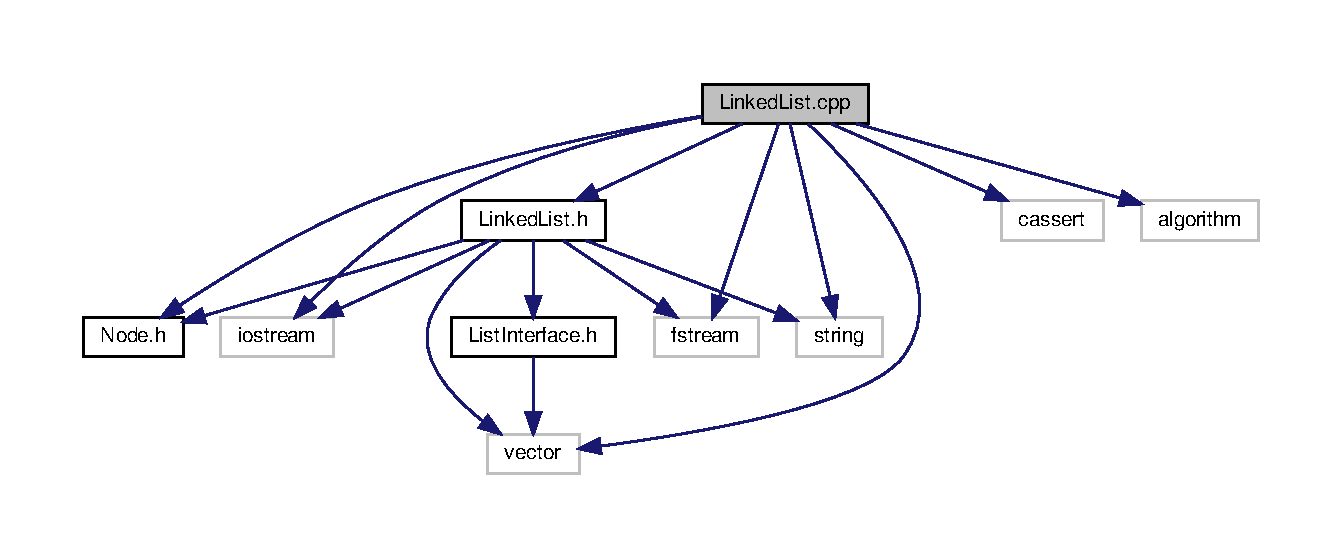
\includegraphics[width=350pt]{LinkedList_8cpp__incl}
\end{center}
\end{figure}
This graph shows which files directly or indirectly include this file\+:\nopagebreak
\begin{figure}[H]
\begin{center}
\leavevmode
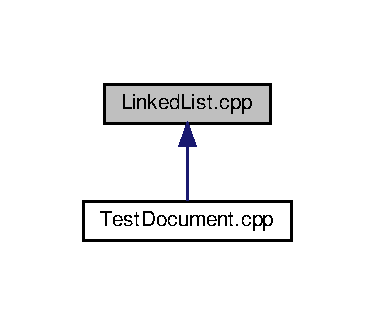
\includegraphics[width=180pt]{LinkedList_8cpp__dep__incl}
\end{center}
\end{figure}

\hypertarget{LinkedList_8cpp_source}{}\section{Linked\+List.\+cpp}

\begin{DoxyCode}
00001 \textcolor{preprocessor}{#include "\hyperlink{LinkedList_8h}{LinkedList.h}"}  \textcolor{comment}{// Header file}
00002 \textcolor{preprocessor}{#include "\hyperlink{Node_8h}{Node.h}"}
00003 \textcolor{comment}{//#include "PrecondViolatedExcep.h"}
00004 \textcolor{preprocessor}{#include <cassert>}
00005 \textcolor{preprocessor}{#include <fstream>}
00006 \textcolor{preprocessor}{#include <iostream>}
00007 \textcolor{preprocessor}{#include <string>}
00008 \textcolor{preprocessor}{#include <vector>}
00009 \textcolor{preprocessor}{#include <algorithm>}
00010   
00011 \textcolor{keyword}{using namespace }\hyperlink{namespacestd}{std};
00012 
00014 
00017 \textcolor{keyword}{template}<\textcolor{keyword}{class} ItemType>
\Hypertarget{LinkedList_8cpp_source_l00018}\hyperlink{classLinkedList_adf8d8164e06b6d358a36df7e53e814ee}{00018} \hyperlink{classLinkedList_adf8d8164e06b6d358a36df7e53e814ee}{LinkedList<ItemType>::LinkedList}() : headPtr(NULL), itemCount(0)
00019 \{
00020 \}  \textcolor{comment}{// end default constructor}
00021 
00023 
00027 \textcolor{keyword}{template}<\textcolor{keyword}{class} ItemType>
\Hypertarget{LinkedList_8cpp_source_l00028}\hyperlink{classLinkedList_a6f1443c6120352f1f5b6bd3c0d95e41e}{00028} \hyperlink{classLinkedList_adf8d8164e06b6d358a36df7e53e814ee}{LinkedList<ItemType>::LinkedList}(\textcolor{keyword}{const} 
      \hyperlink{classLinkedList}{LinkedList<ItemType>}& aList) : itemCount(aList.itemCount)
00029 \{
00030    \hyperlink{classNode}{Node<ItemType>}* origChainPtr = aList.headPtr;  \textcolor{comment}{// Points to nodes in original chain}
00031 
00032    \textcolor{keywordflow}{if} (origChainPtr == NULL)
00033       headPtr = NULL;  \textcolor{comment}{// Original list is empty}
00034    \textcolor{keywordflow}{else}
00035    \{
00036       \textcolor{comment}{// Copy first node}
00037       headPtr = \textcolor{keyword}{new} \hyperlink{classNode}{Node<ItemType>}();
00038       headPtr->setItem(origChainPtr->\hyperlink{classNode_a6c08caef312b6f2f69b5e090cf047514}{getItem}());
00039       
00040       \textcolor{comment}{// Copy remaining nodes}
00041       \hyperlink{classNode}{Node<ItemType>}* newChainPtr = headPtr;      \textcolor{comment}{// Points to last node in new chain}
00042       origChainPtr = origChainPtr->\hyperlink{classNode_a3eb0c96e03a3fd46ea1cff4c305bbedd}{getNext}();     \textcolor{comment}{// Advance original-chain pointer}
00043       \textcolor{keywordflow}{while} (origChainPtr != NULL)
00044       \{
00045          \textcolor{comment}{// Get next item from original chain}
00046          ItemType nextItem = origChainPtr->\hyperlink{classNode_a6c08caef312b6f2f69b5e090cf047514}{getItem}();
00047          
00048          \textcolor{comment}{// Create a new node containing the next item }
00049          \hyperlink{classNode}{Node<ItemType>}* newNodePtr = \textcolor{keyword}{new} \hyperlink{classNode}{Node<ItemType>}(nextItem);  
00050          
00051          \textcolor{comment}{// Link new node to end of new chain}
00052          newChainPtr->\hyperlink{classNode_a01c1a66d4e39f5b149e090413deb4633}{setNext}(newNodePtr); 
00053          
00054          \textcolor{comment}{// Advance pointer to new last node      }
00055          newChainPtr = newChainPtr->\hyperlink{classNode_a3eb0c96e03a3fd46ea1cff4c305bbedd}{getNext}();
00056          
00057          \textcolor{comment}{// Advance original-chain pointer}
00058          origChainPtr = origChainPtr->\hyperlink{classNode_a3eb0c96e03a3fd46ea1cff4c305bbedd}{getNext}();
00059       \}  \textcolor{comment}{// end while}
00060       
00061       newChainPtr->\hyperlink{classNode_a01c1a66d4e39f5b149e090413deb4633}{setNext}(NULL);              \textcolor{comment}{// Flag end of chain}
00062    \}  \textcolor{comment}{// end if}
00063 \}  \textcolor{comment}{// end copy constructor}
00064 
00066 
00069 \textcolor{keyword}{template}<\textcolor{keyword}{class} ItemType>
\Hypertarget{LinkedList_8cpp_source_l00070}\hyperlink{classLinkedList_a66aee17d756fe0e002375897383c180b}{00070} \hyperlink{classLinkedList_a66aee17d756fe0e002375897383c180b}{LinkedList<ItemType>::~LinkedList}()
00071 \{
00072    \hyperlink{classLinkedList_a7d1d9cf83eef67b6c4d700a3cc5970e1}{clear}();
00073 \}  \textcolor{comment}{// end destructor}
00074 
00076 
00080 \textcolor{keyword}{template}<\textcolor{keyword}{class} ItemType>
\Hypertarget{LinkedList_8cpp_source_l00081}\hyperlink{classLinkedList_a008e916c3d51d28b4cc9c8cdf3e9d921}{00081} \textcolor{keywordtype}{bool} \hyperlink{classLinkedList_a008e916c3d51d28b4cc9c8cdf3e9d921}{LinkedList<ItemType>::isEmpty}()\textcolor{keyword}{ const}
00082 \textcolor{keyword}{}\{
00083    \textcolor{keywordflow}{return} itemCount == 0;
00084 \}  \textcolor{comment}{// end isEmpty}
00085 
00087 
00090 \textcolor{keyword}{template}<\textcolor{keyword}{class} ItemType>
\Hypertarget{LinkedList_8cpp_source_l00091}\hyperlink{classLinkedList_a61d045ef6008b494a1a516ecc992c0e7}{00091} \textcolor{keywordtype}{int} \hyperlink{classLinkedList_a61d045ef6008b494a1a516ecc992c0e7}{LinkedList<ItemType>::getLength}()\textcolor{keyword}{ const}
00092 \textcolor{keyword}{}\{
00093    \textcolor{keywordflow}{return} itemCount;
00094 \}  \textcolor{comment}{// end getLength}
00095 
00097 
00105 \textcolor{keyword}{template}<\textcolor{keyword}{class} ItemType>
\Hypertarget{LinkedList_8cpp_source_l00106}\hyperlink{classLinkedList_ae8a19375505e87e2e4fc0e9b5afe4d4d}{00106} \textcolor{keywordtype}{bool} \hyperlink{classLinkedList_ae8a19375505e87e2e4fc0e9b5afe4d4d}{LinkedList<ItemType>::insert}(\textcolor{keywordtype}{int} newPosition, \textcolor{keyword}{const} ItemType& newEntry)
00107 \{
00108    \textcolor{keywordtype}{bool} ableToInsert = (newPosition >= 1) && (newPosition <= itemCount + 1);
00109    \textcolor{keywordflow}{if} (ableToInsert)
00110    \{
00111       \hyperlink{classNode}{Node<ItemType>}* newNodePtr = \textcolor{keyword}{new} \hyperlink{classNode}{Node<ItemType>}(newEntry);  
00112       \textcolor{keywordflow}{if} (newPosition == 1)
00113       \{
00114          newNodePtr->\hyperlink{classNode_a01c1a66d4e39f5b149e090413deb4633}{setNext}(headPtr); 
00115          headPtr = newNodePtr;
00116       \}
00117       \textcolor{keywordflow}{else}
00118       \{
00119          \hyperlink{classNode}{Node<ItemType>}* prevPtr = getNodeAt(newPosition - 1);
00120          newNodePtr->\hyperlink{classNode_a01c1a66d4e39f5b149e090413deb4633}{setNext}(prevPtr->\hyperlink{classNode_a3eb0c96e03a3fd46ea1cff4c305bbedd}{getNext}()); 
00121          prevPtr->\hyperlink{classNode_a01c1a66d4e39f5b149e090413deb4633}{setNext}(newNodePtr);
00122       \}  \textcolor{comment}{// end if}
00123       itemCount++; 
00124    \}  \textcolor{comment}{// end if}
00125    \textcolor{keywordflow}{return} ableToInsert;
00126 \}  \textcolor{comment}{// end inser}
00127 
00128 
00129 \textcolor{comment}{/*}
00130 \textcolor{comment}{template<class ItemType>}
00131 \textcolor{comment}{void LinkedList<ItemType>::remove(int position)}
00132 \textcolor{comment}{\{}
00133 \textcolor{comment}{       bool ableToNull = (position >= 1) && (position <= itemCount);}
00134 \textcolor{comment}{       if (ableToNull)}
00135 \textcolor{comment}{       \{}
00136 \textcolor{comment}{          Node<ItemType>* nodePtr = getNodeAt(position);}
00137 \textcolor{comment}{          nodePtr->setItem(NULL);}
00138 \textcolor{comment}{       \}  // end if}
00139 \textcolor{comment}{    }
00140 \textcolor{comment}{}
00141 \textcolor{comment}{\}  // end remove}
00142 \textcolor{comment}{*/}
00143 
00145 
00150 \textcolor{keyword}{template}<\textcolor{keyword}{class} ItemType>
\Hypertarget{LinkedList_8cpp_source_l00151}\hyperlink{classLinkedList_a7dc3cca217b45c6fe5d28c9d16b7bf9e}{00151} \textcolor{keywordtype}{bool} \hyperlink{classLinkedList_a7dc3cca217b45c6fe5d28c9d16b7bf9e}{LinkedList<ItemType>::deletion}(\textcolor{keywordtype}{int} position)
00152 \{
00153        \textcolor{keywordtype}{bool} ableToRemove = (position >= 1) && (position <= itemCount);
00154        \textcolor{keywordflow}{if} (ableToRemove)
00155        \{
00156           \hyperlink{classNode}{Node<ItemType>}* curPtr = NULL;
00157           \textcolor{keywordflow}{if} (position == 1)
00158           \{
00159              curPtr = headPtr; \textcolor{comment}{// Save pointer to node}
00160              headPtr = headPtr->getNext();
00161           \}
00162           \textcolor{keywordflow}{else}
00163           \{
00164              \hyperlink{classNode}{Node<ItemType>}* prevPtr = getNodeAt(position - 1);
00165              curPtr = prevPtr->\hyperlink{classNode_a3eb0c96e03a3fd46ea1cff4c305bbedd}{getNext}();
00166              prevPtr->\hyperlink{classNode_a01c1a66d4e39f5b149e090413deb4633}{setNext}(curPtr->\hyperlink{classNode_a3eb0c96e03a3fd46ea1cff4c305bbedd}{getNext}());
00167           \}  \textcolor{comment}{// end if}
00168       
00169           curPtr->\hyperlink{classNode_a01c1a66d4e39f5b149e090413deb4633}{setNext}(NULL);
00170           \textcolor{keyword}{delete} curPtr;
00171           curPtr = NULL;
00172           itemCount--; 
00173       
00174  \textcolor{comment}{// Decrease count of entries}
00175    \}  \textcolor{comment}{// end if}
00176    
00177    \textcolor{keywordflow}{return} ableToRemove;
00178 \}  \textcolor{comment}{// end remove}
00179 
00181 
00184 \textcolor{keyword}{template}<\textcolor{keyword}{class} ItemType>
\Hypertarget{LinkedList_8cpp_source_l00185}\hyperlink{classLinkedList_a7d1d9cf83eef67b6c4d700a3cc5970e1}{00185} \textcolor{keywordtype}{void} \hyperlink{classLinkedList_a7d1d9cf83eef67b6c4d700a3cc5970e1}{LinkedList<ItemType>::clear}()
00186 \{
00187    \textcolor{keywordflow}{while} (!\hyperlink{classLinkedList_a008e916c3d51d28b4cc9c8cdf3e9d921}{isEmpty}())
00188       \hyperlink{classLinkedList_a7dc3cca217b45c6fe5d28c9d16b7bf9e}{deletion}(1);
00189 \}  \textcolor{comment}{// end clear}
00190 
00192 
00197 \textcolor{keyword}{template}<\textcolor{keyword}{class} ItemType>
\Hypertarget{LinkedList_8cpp_source_l00198}\hyperlink{classLinkedList_a341bfd7772c9d24d29eb7a7f3936915b}{00198} ItemType \hyperlink{classLinkedList_a341bfd7772c9d24d29eb7a7f3936915b}{LinkedList<ItemType>::getEntry}(\textcolor{keywordtype}{int} position) \textcolor{keyword}{const}\textcolor{comment}{//const
       throw(PrecondViolatedExcep)}
00199 \{
00200    \textcolor{keywordtype}{bool} ableToGet = (position > 0) && (position <= itemCount);
00201    \textcolor{keywordflow}{if} (ableToGet)
00202    \{
00203       \hyperlink{classNode}{Node<ItemType>}* nodePtr = getNodeAt(position);
00204       \textcolor{keywordflow}{return} nodePtr->\hyperlink{classNode_a6c08caef312b6f2f69b5e090cf047514}{getItem}();
00205    \}
00206    \textcolor{keywordflow}{else}
00207    \{
00208        \textcolor{keywordflow}{return} ItemType();
00209        \textcolor{comment}{//throw(PrecondViolatedExcep(message)); }
00210    \}  \textcolor{comment}{// end if}
00211 \}  \textcolor{comment}{// end getEntr}
00212 
00214 
00218 \textcolor{keyword}{template}<\textcolor{keyword}{class} ItemType>
\Hypertarget{LinkedList_8cpp_source_l00219}\hyperlink{classLinkedList_a3035f880c50e7d8f68e67c093d4607ca}{00219} \textcolor{keywordtype}{void} \hyperlink{classLinkedList_a3035f880c50e7d8f68e67c093d4607ca}{LinkedList<ItemType>::replace}(\textcolor{keywordtype}{int} position, \textcolor{keyword}{const} ItemType& newEntry)\textcolor{comment}{//
       throw(PrecondViolatedExcep)}
00220 \{
00221    \textcolor{keywordtype}{bool} ableToSet = (position >= 1) && (position <= itemCount);
00222    \textcolor{keywordflow}{if} (ableToSet)
00223    \{
00224       \hyperlink{classNode}{Node<ItemType>}* nodePtr = getNodeAt(position);
00225       nodePtr->\hyperlink{classNode_ab4ceecdecc5df799011de486b9f54974}{setItem}(newEntry);
00226    \}
00227    \textcolor{keywordflow}{else}
00228    \{
00229       \textcolor{keywordtype}{string} message = \textcolor{stringliteral}{"replace() called with an invalid position."};
00230       \textcolor{comment}{//throw(PrecondViolatedExcep(message)); }
00231    \}  \textcolor{comment}{// end if}
00232 \}  \textcolor{comment}{// end replace}
00233 
00234 
00236 
00243 \textcolor{keyword}{template}<\textcolor{keyword}{class} ItemType>
00244 \hyperlink{classNode}{Node<ItemType>}* \hyperlink{classLinkedList}{LinkedList<ItemType>::getNodeAt}(\textcolor{keywordtype}{int} position)\textcolor{keyword}{
       const}
00245 \textcolor{keyword}{}\{
00246    \textcolor{comment}{// Debugging check of precondition}
00247    assert( (position >= 1) && (position <= itemCount) );
00248    
00249    \textcolor{comment}{// Count from the beginning of the chain}
00250    \hyperlink{classNode}{Node<ItemType>}* curPtr = headPtr;
00251    \textcolor{keywordflow}{for} (\textcolor{keywordtype}{int} skip = 1; skip < position; skip++)
00252       curPtr = curPtr->\hyperlink{classNode_a3eb0c96e03a3fd46ea1cff4c305bbedd}{getNext}();
00253       
00254    \textcolor{keywordflow}{return} curPtr;
00255 \}  \textcolor{comment}{// end getNodeAt}
00256 \textcolor{comment}{//  End of implementation file.}
00257 
00259 
00262 \textcolor{keyword}{template}<\textcolor{keyword}{class} ItemType>
\Hypertarget{LinkedList_8cpp_source_l00263}\hyperlink{classLinkedList_afc6635f854f48f2f126cf3b60d845220}{00263} \textcolor{keywordtype}{int} \hyperlink{classLinkedList_afc6635f854f48f2f126cf3b60d845220}{LinkedList<ItemType>::getItemCount}()\textcolor{keyword}{ const}
00264 \textcolor{keyword}{}\{
00265     \textcolor{keywordflow}{return} itemCount;
00266 \}
00267 
00269 
00273 \textcolor{keyword}{template}<\textcolor{keyword}{class} ItemType>
\Hypertarget{LinkedList_8cpp_source_l00274}\hyperlink{classLinkedList_a65fb58d9f9b8af41e9569d1dc3200583}{00274} ItemType \hyperlink{classLinkedList_a65fb58d9f9b8af41e9569d1dc3200583}{LinkedList<ItemType>::displayList}()
00275 \{
00276     \textcolor{keywordflow}{for} (\textcolor{keywordtype}{int} i = 0; i > itemCount; i++)
00277     \{
00278         \hyperlink{classNode}{Node<ItemType>}* nodePtr = getNodeAt(i);
00279         \textcolor{keywordflow}{return} nodePtr->\hyperlink{classNode_a6c08caef312b6f2f69b5e090cf047514}{getItem}();
00280     \}
00281 \}
00282 
00284 
00288 \textcolor{keyword}{template}<\textcolor{keyword}{class} ItemType>
\Hypertarget{LinkedList_8cpp_source_l00289}\hyperlink{classLinkedList_a25b0fba69e66b0fa409be992530029bc}{00289} \hyperlink{classLinkedList}{LinkedList<ItemType>}& \hyperlink{classLinkedList_a25b0fba69e66b0fa409be992530029bc}{LinkedList<ItemType>::operator = }
      (\textcolor{keyword}{const} \hyperlink{classLinkedList}{LinkedList<ItemType>}& rhs) 
00290 \{
00291     \hyperlink{classLinkedList}{LinkedList<ItemType>} temp(rhs);
00292     swap(temp.headPtr, headPtr);
00293     \textcolor{keywordflow}{return} *\textcolor{keyword}{this};
00294 \}
\end{DoxyCode}

\hypertarget{LinkedList_8h}{}\section{Linked\+List.\+h File Reference}
\label{LinkedList_8h}\index{Linked\+List.\+h@{Linked\+List.\+h}}
{\ttfamily \#include \char`\"{}List\+Interface.\+h\char`\"{}}\newline
{\ttfamily \#include \char`\"{}Node.\+h\char`\"{}}\newline
{\ttfamily \#include $<$iostream$>$}\newline
{\ttfamily \#include $<$fstream$>$}\newline
{\ttfamily \#include $<$string$>$}\newline
{\ttfamily \#include $<$vector$>$}\newline
Include dependency graph for Linked\+List.\+h\+:\nopagebreak
\begin{figure}[H]
\begin{center}
\leavevmode
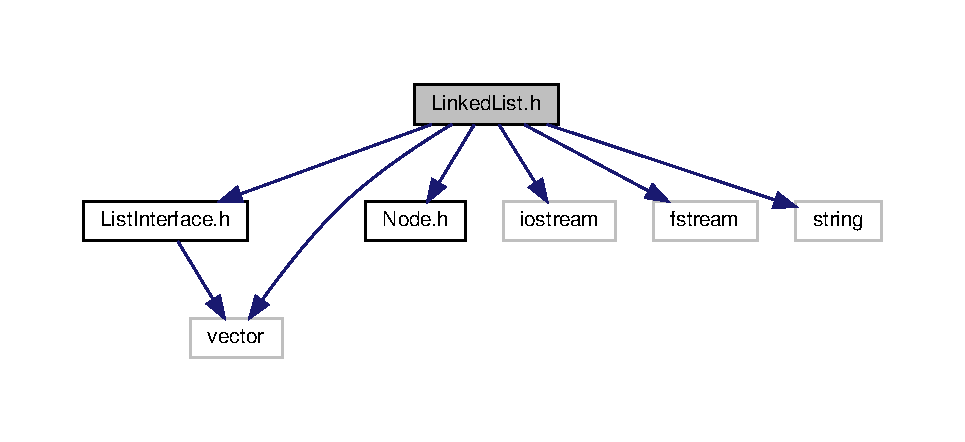
\includegraphics[width=350pt]{LinkedList_8h__incl}
\end{center}
\end{figure}
This graph shows which files directly or indirectly include this file\+:\nopagebreak
\begin{figure}[H]
\begin{center}
\leavevmode
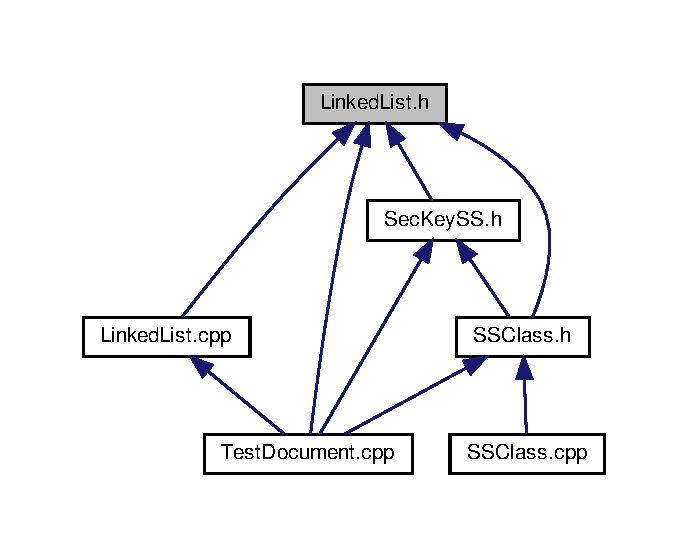
\includegraphics[width=330pt]{LinkedList_8h__dep__incl}
\end{center}
\end{figure}
\subsection*{Classes}
\begin{DoxyCompactItemize}
\item 
class \hyperlink{classLinkedList}{Linked\+List$<$ Item\+Type $>$}
\begin{DoxyCompactList}\small\item\em This is \hyperlink{classLinkedList}{Linked\+List} class creating a list of linked nodes. \end{DoxyCompactList}\end{DoxyCompactItemize}

\hypertarget{LinkedList_8h_source}{}\section{Linked\+List.\+h}

\begin{DoxyCode}
00001 \textcolor{comment}{/***************************************************************************/}
00008 \textcolor{preprocessor}{#ifndef LINKED\_LIST\_}
00009 \textcolor{preprocessor}{#define LINKED\_LIST\_}
00010 
00011 \textcolor{preprocessor}{#include "\hyperlink{ListInterface_8h}{ListInterface.h}"}
00012 \textcolor{preprocessor}{#include "\hyperlink{Node_8h}{Node.h}"}
00013 \textcolor{preprocessor}{#include <iostream>}
00014 \textcolor{preprocessor}{#include <fstream>}
00015 \textcolor{preprocessor}{#include <string>}
00016 \textcolor{preprocessor}{#include <vector>}
00017 
00018 \textcolor{keyword}{template}<\textcolor{keyword}{class} ItemType>
\Hypertarget{LinkedList_8h_source_l00019}\hyperlink{classLinkedList}{00019} \textcolor{keyword}{class }\hyperlink{classLinkedList}{LinkedList} : \textcolor{keyword}{public} \hyperlink{classListInterface}{ListInterface}<ItemType>
00020 \{
00021 \textcolor{keyword}{private}:
00022    \hyperlink{classNode}{Node<ItemType>}* headPtr; \textcolor{comment}{// Pointer to first node in the chain;}
00023    \textcolor{comment}{// (contains the first entry in the list)}
00024    \textcolor{keywordtype}{int} itemCount; \textcolor{comment}{// Current count of list items   }
00025    \textcolor{comment}{// Locates a specified node in this linked list.}
00026    \textcolor{comment}{// @pre  position is the number of the desired node;}
00027    \textcolor{comment}{//       position >= 1 and position <= itemCount.}
00028    \textcolor{comment}{// @post  The node is found and a pointer to it is returned.}
00029    \textcolor{comment}{// @param position  The number of the node to locate.}
00030    \textcolor{comment}{// @return  A pointer to the node at the given position.}
00031    \hyperlink{classNode}{Node<ItemType>}* getNodeAt(\textcolor{keywordtype}{int} position) \textcolor{keyword}{const};
00032    
00033 \textcolor{keyword}{public}:
00034    \hyperlink{classLinkedList_adf8d8164e06b6d358a36df7e53e814ee}{LinkedList}();
00035    \hyperlink{classLinkedList_adf8d8164e06b6d358a36df7e53e814ee}{LinkedList}(\textcolor{keyword}{const} \hyperlink{classLinkedList}{LinkedList<ItemType>}& aList);
00036    \textcolor{keyword}{virtual} \hyperlink{classLinkedList_a66aee17d756fe0e002375897383c180b}{~LinkedList}();
00037 
00038    
00039    \textcolor{keywordtype}{bool} \hyperlink{classLinkedList_a008e916c3d51d28b4cc9c8cdf3e9d921}{isEmpty}() \textcolor{keyword}{const};
00040    \textcolor{keywordtype}{int} \hyperlink{classLinkedList_a61d045ef6008b494a1a516ecc992c0e7}{getLength}() \textcolor{keyword}{const};
00041    \textcolor{keywordtype}{bool} \hyperlink{classLinkedList_ae8a19375505e87e2e4fc0e9b5afe4d4d}{insert}(\textcolor{keywordtype}{int} newPosition, \textcolor{keyword}{const} ItemType& newEntry);
00042    \textcolor{comment}{//void remove(int position);}
00043    \textcolor{keywordtype}{bool} \hyperlink{classLinkedList_a7dc3cca217b45c6fe5d28c9d16b7bf9e}{deletion}(\textcolor{keywordtype}{int} position);
00044    \textcolor{keywordtype}{void} \hyperlink{classLinkedList_a7d1d9cf83eef67b6c4d700a3cc5970e1}{clear}();
00045    \textcolor{keywordtype}{int} \hyperlink{classLinkedList_afc6635f854f48f2f126cf3b60d845220}{getItemCount}() \textcolor{keyword}{const};
00046    \hyperlink{classLinkedList}{LinkedList<ItemType>}& \hyperlink{classLinkedList_a25b0fba69e66b0fa409be992530029bc}{operator = }(\textcolor{keyword}{const} 
      \hyperlink{classLinkedList}{LinkedList<ItemType>}& rhs);
00047 
00050    ItemType \hyperlink{classLinkedList_a341bfd7772c9d24d29eb7a7f3936915b}{getEntry}(\textcolor{keywordtype}{int} position) \textcolor{keyword}{const}; 
00051 
00054    \textcolor{keywordtype}{void} \hyperlink{classLinkedList_a3035f880c50e7d8f68e67c093d4607ca}{replace}(\textcolor{keywordtype}{int} position, \textcolor{keyword}{const} ItemType &newEntry); 
00055 
00056    ItemType \hyperlink{classLinkedList_a65fb58d9f9b8af41e9569d1dc3200583}{displayList}();
00057 
00058 
00059 
00060 \}; \textcolor{comment}{// end LinkedList}
00061 
00062 \textcolor{comment}{//#include "LinkedList.cpp"}
00063 \textcolor{preprocessor}{#endif }
\end{DoxyCode}

\hypertarget{ListInterface_8h}{}\section{List\+Interface.\+h File Reference}
\label{ListInterface_8h}\index{List\+Interface.\+h@{List\+Interface.\+h}}
{\ttfamily \#include $<$vector$>$}\newline
Include dependency graph for List\+Interface.\+h\+:\nopagebreak
\begin{figure}[H]
\begin{center}
\leavevmode
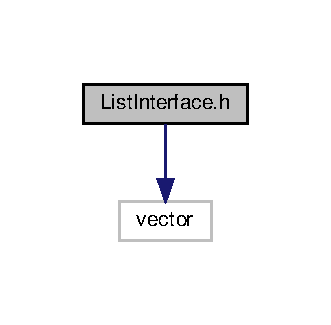
\includegraphics[width=159pt]{ListInterface_8h__incl}
\end{center}
\end{figure}
This graph shows which files directly or indirectly include this file\+:\nopagebreak
\begin{figure}[H]
\begin{center}
\leavevmode
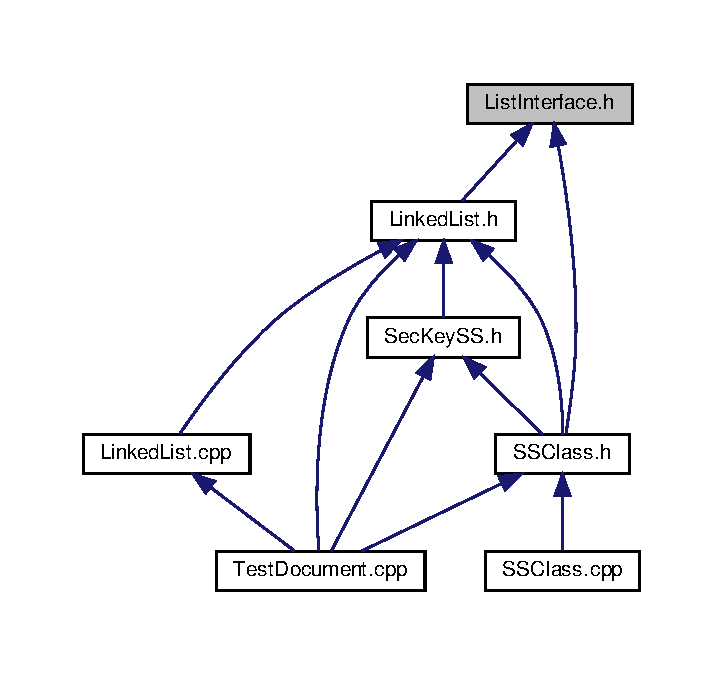
\includegraphics[width=347pt]{ListInterface_8h__dep__incl}
\end{center}
\end{figure}
\subsection*{Classes}
\begin{DoxyCompactItemize}
\item 
class \hyperlink{classListInterface}{List\+Interface$<$ Item\+Type $>$}
\end{DoxyCompactItemize}

\hypertarget{ListInterface_8h_source}{}\section{List\+Interface.\+h}

\begin{DoxyCode}
00001 \textcolor{preprocessor}{#include <vector>}
00002 
00003 \textcolor{preprocessor}{#ifndef \_LIST\_INTERFACE}
00004 \textcolor{preprocessor}{#define \_LIST\_INTERFACE}
00005 
00006 \textcolor{keyword}{template}<\textcolor{keyword}{class} ItemType>
\Hypertarget{ListInterface_8h_source_l00007}\hyperlink{classListInterface}{00007} \textcolor{keyword}{class }\hyperlink{classListInterface}{ListInterface}
00008 \{
00009 \textcolor{keyword}{public}:
00012    \textcolor{keyword}{virtual} \textcolor{keywordtype}{bool} \hyperlink{classListInterface_a924f91e7f81d7dcd3fda79bbcc671394}{isEmpty}() \textcolor{keyword}{const} = 0;
00013    
00016    \textcolor{keyword}{virtual} \textcolor{keywordtype}{int} \hyperlink{classListInterface_afc85695d4137f1e29ff02e179c9f3221}{getLength}() \textcolor{keyword}{const} = 0;
00017    \textcolor{keyword}{virtual} \textcolor{keywordtype}{int} \hyperlink{classListInterface_a3e085e6ea9c5dc3e8007010cd889159c}{getItemCount}() \textcolor{keyword}{const} = 0;
00027    \textcolor{keyword}{virtual} \textcolor{keywordtype}{bool} \hyperlink{classListInterface_a5b2f86954a86172699a3495982c38e77}{insert}(\textcolor{keywordtype}{int} newPosition, \textcolor{keyword}{const} ItemType& newEntry) = 0;
00028 
00029    \textcolor{comment}{//virtual void remove(int position);}
00037 \textcolor{comment}{}   \textcolor{comment}{//virtual void remove(int position) = 0;}
00038    \textcolor{keyword}{virtual} \textcolor{keywordtype}{bool} \hyperlink{classListInterface_a68520ce2942ec716c745b1137c50a3c6}{deletion}(\textcolor{keywordtype}{int} position) = 0;
00041    \textcolor{keyword}{virtual} \textcolor{keywordtype}{void} \hyperlink{classListInterface_adfda414908b645bdf19bcab8269168b7}{clear}() = 0;
00042    
00048    \textcolor{keyword}{virtual} ItemType \hyperlink{classListInterface_a86987f69e5056d287212ede41db1956a}{getEntry}(\textcolor{keywordtype}{int} position) \textcolor{keyword}{const} = 0;
00049    
00055    \textcolor{keyword}{virtual} \textcolor{keywordtype}{void} \hyperlink{classListInterface_aae877a56b7b9f5f526c37a00e234fad1}{replace}(\textcolor{keywordtype}{int} position, \textcolor{keyword}{const} ItemType& newEntry) = 0;
00056 
00057    \textcolor{keyword}{virtual} ItemType \hyperlink{classListInterface_a2f2f533e962dd89111ee50b972dc28e7}{displayList}() = 0;
00058 \}; \textcolor{comment}{// end ListInterface}
00059 \textcolor{preprocessor}{#endif}
\end{DoxyCode}

\hypertarget{Node_8cpp}{}\section{Node.\+cpp File Reference}
\label{Node_8cpp}\index{Node.\+cpp@{Node.\+cpp}}
{\ttfamily \#include \char`\"{}Node.\+h\char`\"{}}\newline
Include dependency graph for Node.\+cpp\+:\nopagebreak
\begin{figure}[H]
\begin{center}
\leavevmode
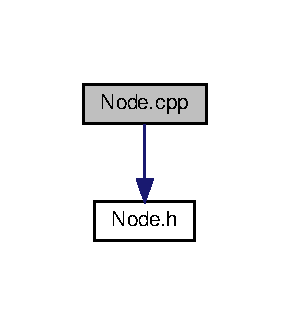
\includegraphics[width=139pt]{Node_8cpp__incl}
\end{center}
\end{figure}
This graph shows which files directly or indirectly include this file\+:\nopagebreak
\begin{figure}[H]
\begin{center}
\leavevmode
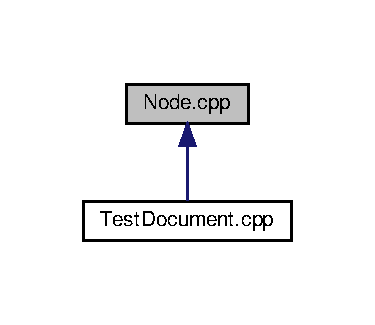
\includegraphics[width=180pt]{Node_8cpp__dep__incl}
\end{center}
\end{figure}

\hypertarget{Node_8cpp_source}{}\section{Node.\+cpp}

\begin{DoxyCode}
00001 \textcolor{preprocessor}{#include "\hyperlink{Node_8h}{Node.h}"}
00002 
00004 
00007 \textcolor{keyword}{template}<\textcolor{keyword}{class} ItemType>
\Hypertarget{Node_8cpp_source_l00008}\hyperlink{classNode_a627e94f4fba0e73c546e0fb2a7266f36}{00008} \hyperlink{classNode_a627e94f4fba0e73c546e0fb2a7266f36}{Node<ItemType>::Node}() : next(nullptr)
00009 \{
00010 \} \textcolor{comment}{// end default constructor}
00011 
00013 
00017 \textcolor{keyword}{template}<\textcolor{keyword}{class} ItemType>
\Hypertarget{Node_8cpp_source_l00018}\hyperlink{classNode_a0288598fcb0244739ce95099c26250ae}{00018} \hyperlink{classNode_a627e94f4fba0e73c546e0fb2a7266f36}{Node<ItemType>::Node}(\textcolor{keyword}{const} ItemType& anItem) : item(anItem), next(nullptr)
00019 \{
00020 \} \textcolor{comment}{// end constructor}
00021 
00023 
00029 \textcolor{keyword}{template}<\textcolor{keyword}{class} ItemType>
\Hypertarget{Node_8cpp_source_l00030}\hyperlink{classNode_adf98d3f9b7227622cb5a0fdd7e8f0b18}{00030} \hyperlink{classNode_a627e94f4fba0e73c546e0fb2a7266f36}{Node<ItemType>::Node}(\textcolor{keyword}{const} ItemType& anItem, \hyperlink{classNode}{Node<ItemType>}* nextNodePtr)
       :
00031     item(anItem), next(nextNodePtr)
00032 \{
00033 \} \textcolor{comment}{// end constructor}
00034 
00036 
00039 \textcolor{keyword}{template}<\textcolor{keyword}{class} ItemType>
\Hypertarget{Node_8cpp_source_l00040}\hyperlink{classNode_ab4ceecdecc5df799011de486b9f54974}{00040} \textcolor{keywordtype}{void} \hyperlink{classNode_ab4ceecdecc5df799011de486b9f54974}{Node<ItemType>::setItem}(\textcolor{keyword}{const} ItemType& anItem)
00041 \{
00042     item = anItem;
00043 \} \textcolor{comment}{// end setItem}
00044 
00046 
00049 \textcolor{keyword}{template}<\textcolor{keyword}{class} ItemType>
\Hypertarget{Node_8cpp_source_l00050}\hyperlink{classNode_a01c1a66d4e39f5b149e090413deb4633}{00050} \textcolor{keywordtype}{void} \hyperlink{classNode_a01c1a66d4e39f5b149e090413deb4633}{Node<ItemType>::setNext}(\hyperlink{classNode}{Node<ItemType>}* nextNodePtr)
00051 \{
00052     next = nextNodePtr;
00053 \} \textcolor{comment}{// end setNext}
00054 
00056 
00059 \textcolor{keyword}{template}<\textcolor{keyword}{class} ItemType>
\Hypertarget{Node_8cpp_source_l00060}\hyperlink{classNode_a6c08caef312b6f2f69b5e090cf047514}{00060} ItemType \hyperlink{classNode_a6c08caef312b6f2f69b5e090cf047514}{Node<ItemType>::getItem}()\textcolor{keyword}{ const}
00061 \textcolor{keyword}{}\{
00062     \textcolor{keywordflow}{return} item;
00063 \} \textcolor{comment}{// end getItem}
00064 
00066 
00069 \textcolor{keyword}{template}<\textcolor{keyword}{class} ItemType>
\Hypertarget{Node_8cpp_source_l00070}\hyperlink{classNode_a3eb0c96e03a3fd46ea1cff4c305bbedd}{00070} \hyperlink{classNode}{Node<ItemType>}* \hyperlink{classNode_a3eb0c96e03a3fd46ea1cff4c305bbedd}{Node<ItemType>::getNext}()\textcolor{keyword}{ const}
00071 \textcolor{keyword}{}\{
00072     \textcolor{keywordflow}{return} next;
00073 \} \textcolor{comment}{// end getNext}
\end{DoxyCode}

\hypertarget{Node_8h}{}\section{Node.\+h File Reference}
\label{Node_8h}\index{Node.\+h@{Node.\+h}}
This graph shows which files directly or indirectly include this file\+:\nopagebreak
\begin{figure}[H]
\begin{center}
\leavevmode
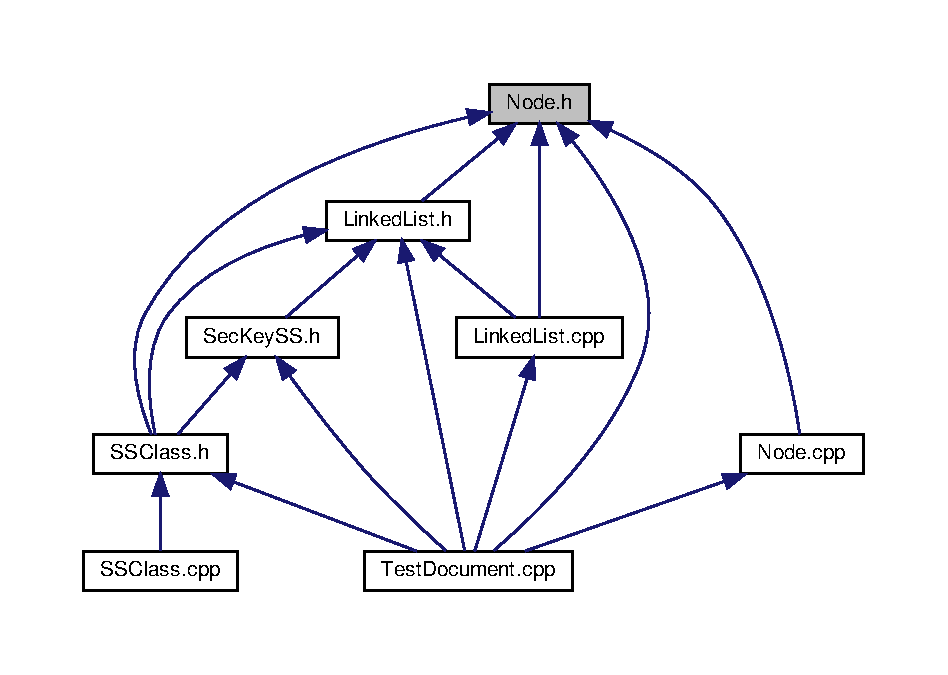
\includegraphics[width=350pt]{Node_8h__dep__incl}
\end{center}
\end{figure}
\subsection*{Classes}
\begin{DoxyCompactItemize}
\item 
class \hyperlink{classNode}{Node$<$ Item\+Type $>$}
\begin{DoxyCompactList}\small\item\em This is \hyperlink{classNode}{Node} class for linked list. \end{DoxyCompactList}\end{DoxyCompactItemize}

\hypertarget{Node_8h_source}{}\section{Node.\+h}

\begin{DoxyCode}
00001 \textcolor{comment}{/***************************************************************************/}
00008 \textcolor{preprocessor}{#ifndef NODE\_}
00009 \textcolor{preprocessor}{#define NODE\_}
00010 
00011 \textcolor{keyword}{template}<\textcolor{keyword}{class} ItemType>
\Hypertarget{Node_8h_source_l00012}\hyperlink{classNode}{00012} \textcolor{keyword}{class }\hyperlink{classNode}{Node}
00013 \{
00014 \textcolor{keyword}{private}:
00015    ItemType        item; \textcolor{comment}{// A data item}
00016    \hyperlink{classNode}{Node<ItemType>}* next; \textcolor{comment}{// Pointer to next node}
00017    
00018 \textcolor{keyword}{public}:      
00019    \hyperlink{classNode_a627e94f4fba0e73c546e0fb2a7266f36}{Node}();
00020    \hyperlink{classNode_a627e94f4fba0e73c546e0fb2a7266f36}{Node}(\textcolor{keyword}{const} ItemType& anItem);
00021    \hyperlink{classNode_a627e94f4fba0e73c546e0fb2a7266f36}{Node}(\textcolor{keyword}{const} ItemType& anItem, \hyperlink{classNode}{Node<ItemType>}* nextNodePtr);
00022    \textcolor{keywordtype}{void} \hyperlink{classNode_ab4ceecdecc5df799011de486b9f54974}{setItem}(\textcolor{keyword}{const} ItemType& anItem);
00023    \textcolor{keywordtype}{void} \hyperlink{classNode_a01c1a66d4e39f5b149e090413deb4633}{setNext}(\hyperlink{classNode}{Node<ItemType>}* nextNodePtr);
00024    ItemType \hyperlink{classNode_a6c08caef312b6f2f69b5e090cf047514}{getItem}() \textcolor{keyword}{const} ;
00025    \hyperlink{classNode}{Node<ItemType>}* \hyperlink{classNode_a3eb0c96e03a3fd46ea1cff4c305bbedd}{getNext}() \textcolor{keyword}{const} ;
00026 \}; \textcolor{comment}{// end Node}
00027 
00028 \textcolor{comment}{//#include "Node.cpp"}
00029 \textcolor{preprocessor}{#endif}
\end{DoxyCode}

\hypertarget{README_8md}{}\section{R\+E\+A\+D\+M\+E.\+md File Reference}
\label{README_8md}\index{R\+E\+A\+D\+M\+E.\+md@{R\+E\+A\+D\+M\+E.\+md}}

\hypertarget{README_8md_source}{}\section{R\+E\+A\+D\+M\+E.\+md}

\begin{DoxyCode}
00001 # CSCI331Project
00002 Github for the CSCI 331 Sequence Set Class Group Programming Project 
\end{DoxyCode}

\hypertarget{SecKeySS_8h}{}\section{Sec\+Key\+S\+S.\+h File Reference}
\label{SecKeySS_8h}\index{Sec\+Key\+S\+S.\+h@{Sec\+Key\+S\+S.\+h}}
{\ttfamily \#include \char`\"{}Linked\+List.\+h\char`\"{}}\newline
Include dependency graph for Sec\+Key\+S\+S.\+h\+:\nopagebreak
\begin{figure}[H]
\begin{center}
\leavevmode
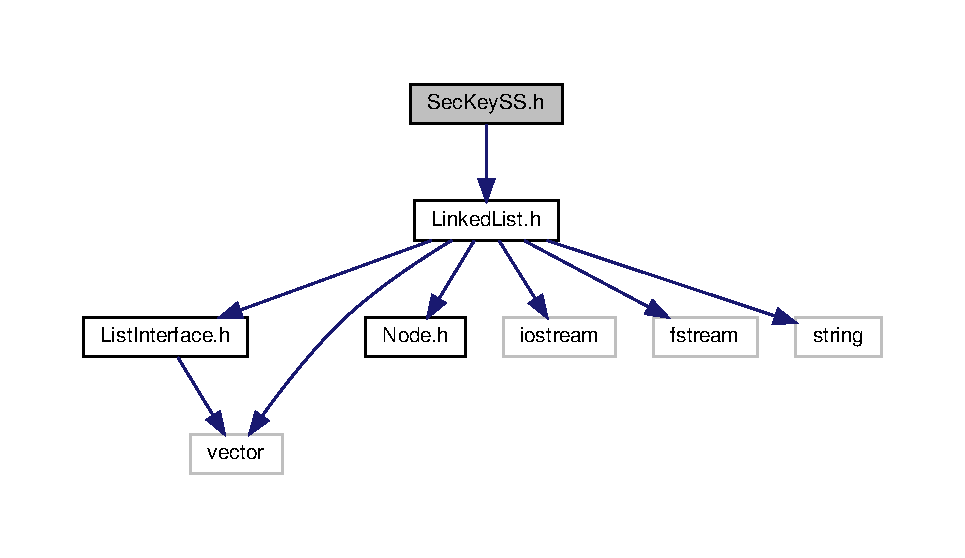
\includegraphics[width=350pt]{SecKeySS_8h__incl}
\end{center}
\end{figure}
This graph shows which files directly or indirectly include this file\+:\nopagebreak
\begin{figure}[H]
\begin{center}
\leavevmode
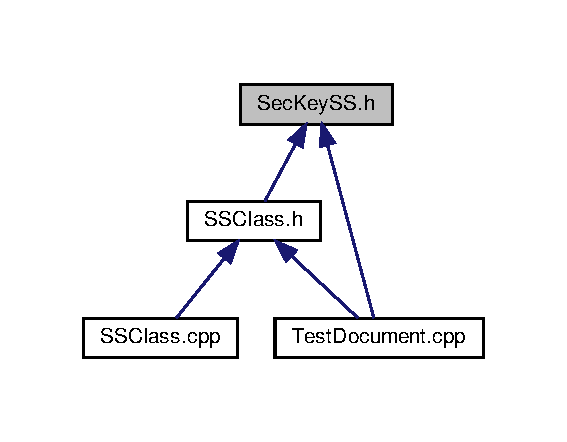
\includegraphics[width=272pt]{SecKeySS_8h__dep__incl}
\end{center}
\end{figure}
\subsection*{Classes}
\begin{DoxyCompactItemize}
\item 
class \hyperlink{classSecKeySS}{Sec\+Key\+S\+S$<$ T $>$}
\begin{DoxyCompactList}\small\item\em This is the class for Section Keys of the SS class. \end{DoxyCompactList}\end{DoxyCompactItemize}
\subsection*{Functions}
\begin{DoxyCompactItemize}
\item 
{\footnotesize template$<$typename T $>$ }\\bool \hyperlink{SecKeySS_8h_a242be966939216bfc391883fbaf6b580}{operator$<$} (const T s1, \hyperlink{classSecKeySS}{Sec\+Key\+SS}$<$ T $>$ \&s2)
\item 
{\footnotesize template$<$typename T $>$ }\\bool \hyperlink{SecKeySS_8h_a4a6ce8378114d62c4438e007eb02dd59}{operator$>$} (const T s1, \hyperlink{classSecKeySS}{Sec\+Key\+SS}$<$ T $>$ s2)
\item 
{\footnotesize template$<$typename T $>$ }\\bool \hyperlink{SecKeySS_8h_a38938ffedfa91568328ae9fef2a2bd02}{operator==} (const T s1, \hyperlink{classSecKeySS}{Sec\+Key\+SS}$<$ T $>$ s2)
\end{DoxyCompactItemize}


\subsection{Function Documentation}
\mbox{\Hypertarget{SecKeySS_8h_a242be966939216bfc391883fbaf6b580}\label{SecKeySS_8h_a242be966939216bfc391883fbaf6b580}} 
\index{Sec\+Key\+S\+S.\+h@{Sec\+Key\+S\+S.\+h}!operator$<$@{operator$<$}}
\index{operator$<$@{operator$<$}!Sec\+Key\+S\+S.\+h@{Sec\+Key\+S\+S.\+h}}
\subsubsection{\texorpdfstring{operator$<$()}{operator<()}}
{\footnotesize\ttfamily template$<$typename T $>$ \\
bool operator$<$ (\begin{DoxyParamCaption}\item[{const T}]{s1,  }\item[{\hyperlink{classSecKeySS}{Sec\+Key\+SS}$<$ T $>$ \&}]{s2 }\end{DoxyParamCaption})}



Definition at line \hyperlink{SecKeySS_8h_source_l00113}{113} of file \hyperlink{SecKeySS_8h_source}{Sec\+Key\+S\+S.\+h}.

\mbox{\Hypertarget{SecKeySS_8h_a38938ffedfa91568328ae9fef2a2bd02}\label{SecKeySS_8h_a38938ffedfa91568328ae9fef2a2bd02}} 
\index{Sec\+Key\+S\+S.\+h@{Sec\+Key\+S\+S.\+h}!operator==@{operator==}}
\index{operator==@{operator==}!Sec\+Key\+S\+S.\+h@{Sec\+Key\+S\+S.\+h}}
\subsubsection{\texorpdfstring{operator==()}{operator==()}}
{\footnotesize\ttfamily template$<$typename T $>$ \\
bool operator== (\begin{DoxyParamCaption}\item[{const T}]{s1,  }\item[{\hyperlink{classSecKeySS}{Sec\+Key\+SS}$<$ T $>$}]{s2 }\end{DoxyParamCaption})}



Definition at line \hyperlink{SecKeySS_8h_source_l00121}{121} of file \hyperlink{SecKeySS_8h_source}{Sec\+Key\+S\+S.\+h}.

\mbox{\Hypertarget{SecKeySS_8h_a4a6ce8378114d62c4438e007eb02dd59}\label{SecKeySS_8h_a4a6ce8378114d62c4438e007eb02dd59}} 
\index{Sec\+Key\+S\+S.\+h@{Sec\+Key\+S\+S.\+h}!operator$>$@{operator$>$}}
\index{operator$>$@{operator$>$}!Sec\+Key\+S\+S.\+h@{Sec\+Key\+S\+S.\+h}}
\subsubsection{\texorpdfstring{operator$>$()}{operator>()}}
{\footnotesize\ttfamily template$<$typename T $>$ \\
bool operator$>$ (\begin{DoxyParamCaption}\item[{const T}]{s1,  }\item[{\hyperlink{classSecKeySS}{Sec\+Key\+SS}$<$ T $>$}]{s2 }\end{DoxyParamCaption})}



Definition at line \hyperlink{SecKeySS_8h_source_l00117}{117} of file \hyperlink{SecKeySS_8h_source}{Sec\+Key\+S\+S.\+h}.


\hypertarget{SecKeySS_8h_source}{}\section{Sec\+Key\+S\+S.\+h}

\begin{DoxyCode}
00001 
00006 \textcolor{preprocessor}{#ifndef SECKEYSS}
00007 \textcolor{preprocessor}{#define SECKEYSS}
00008 
00009 \textcolor{preprocessor}{#include "\hyperlink{LinkedList_8h}{LinkedList.h}"}
00010 \textcolor{comment}{//#include <string>}
00011 
00012 \textcolor{keyword}{using namespace }\hyperlink{namespacestd}{std};
00013 \textcolor{keyword}{template} <\textcolor{keyword}{typename} T>
\Hypertarget{SecKeySS_8h_source_l00014}\hyperlink{classSecKeySS}{00014} \textcolor{keyword}{class }\hyperlink{classSecKeySS}{SecKeySS} \{
00015 \textcolor{keyword}{private}:
00016     T data;
00017     \hyperlink{classLinkedList}{LinkedList<T>} duplicates;
00018     \hyperlink{classLinkedList}{LinkedList<T>} list;
00019 \textcolor{keyword}{public}:
00021     \textcolor{comment}{//template <typename T>}
\Hypertarget{SecKeySS_8h_source_l00022}\hyperlink{classSecKeySS_a9f905dffce0987d620cb2883b3f774cc}{00022}     \hyperlink{classSecKeySS_a9f905dffce0987d620cb2883b3f774cc}{SecKeySS}() \{ duplicates = \hyperlink{classLinkedList}{LinkedList<T>}(); \};
00023     
00025 \textcolor{comment}{//  template <typename T>}
00026     \hyperlink{classSecKeySS}{SecKeySS}( \hyperlink{classSecKeySS}{SecKeySS<T>}& s);
00027 
00029 \textcolor{comment}{//  template <typename T>}
00030     ~\hyperlink{classSecKeySS}{SecKeySS}();
00031 
00035 \textcolor{comment}{//  template <typename T>}
\Hypertarget{SecKeySS_8h_source_l00036}\hyperlink{classSecKeySS_a9fdb8a771250b7aaab556f019b381eab}{00036}     T \hyperlink{classSecKeySS_a9fdb8a771250b7aaab556f019b381eab}{getData}()\textcolor{keyword}{ const }\{ \textcolor{keywordflow}{return} data; \};
00037 
00041     \textcolor{comment}{//template <typename T>}
00042     \hyperlink{classLinkedList}{LinkedList<T>} getDuplicates() ;
00043 
00047 \textcolor{comment}{//  template <typename T>}
\Hypertarget{SecKeySS_8h_source_l00048}\hyperlink{classSecKeySS_ae893fbaf619bf61f73f1585ae5686609}{00048}     \textcolor{keywordtype}{void} \hyperlink{classSecKeySS_ae893fbaf619bf61f73f1585ae5686609}{setData}(\textcolor{keyword}{const} T s) \{ data = s; \};
00049 
00053 \textcolor{comment}{//  template <typename T>}
00054     \textcolor{keywordtype}{void} setDuplicates( \hyperlink{classLinkedList}{LinkedList<T>} dup);
00055 
00060 \textcolor{comment}{//  template <typename T>}
\Hypertarget{SecKeySS_8h_source_l00061}\hyperlink{classSecKeySS_a4a77c5d5b609ef01c17f82001e9f1a7b}{00061}     \textcolor{keywordtype}{bool} \hyperlink{SecKeySS_8h_a242be966939216bfc391883fbaf6b580}{operator <}(\textcolor{keyword}{const} T &s)\textcolor{keyword}{const }\{ \textcolor{keywordflow}{return} data < s; \};
00062 
00063 
00068 \textcolor{comment}{//  template <typename T>}
\Hypertarget{SecKeySS_8h_source_l00069}\hyperlink{classSecKeySS_ae39c46934a033ff213c1d1a7a32cd2bf}{00069}     \textcolor{keywordtype}{bool} operator <(const SecKeySS<T>& s)\textcolor{keyword}{const} \{ \textcolor{keywordflow}{return} data < s.data; \};
00070 
00071 
00076 \textcolor{comment}{//  template <typename T>}
\Hypertarget{SecKeySS_8h_source_l00077}\hyperlink{classSecKeySS_a31bd2d2a2d8eeed14d478cbe88365843}{00077}     \textcolor{keywordtype}{bool} \hyperlink{SecKeySS_8h_a4a6ce8378114d62c4438e007eb02dd59}{operator >}(\textcolor{keyword}{const} T &s)\textcolor{keyword}{const }\{ \textcolor{keywordflow}{return} data > s; \};
00078 
00079 
00084 \textcolor{comment}{//  template <typename T>}
\Hypertarget{SecKeySS_8h_source_l00085}\hyperlink{classSecKeySS_a5c5416d15e14212627b1076644abbb42}{00085}     \textcolor{keywordtype}{bool} \hyperlink{SecKeySS_8h_a4a6ce8378114d62c4438e007eb02dd59}{operator >}(\textcolor{keyword}{const} \hyperlink{classSecKeySS}{SecKeySS<T>} &s)\textcolor{keyword}{const }\{ \textcolor{keywordflow}{return} data > s.data; \};
00086 
00091 \textcolor{comment}{//  template <typename T>}
\Hypertarget{SecKeySS_8h_source_l00092}\hyperlink{classSecKeySS_ace15e2f5c729c58526f97919aff33036}{00092}     \textcolor{keywordtype}{bool} \hyperlink{SecKeySS_8h_a38938ffedfa91568328ae9fef2a2bd02}{operator ==}(\textcolor{keyword}{const} T &s)\textcolor{keyword}{const }\{ \textcolor{keywordflow}{return} data == s; \};
00093 
00094 
00099 \textcolor{comment}{//  template <typename T>}
\Hypertarget{SecKeySS_8h_source_l00100}\hyperlink{classSecKeySS_abf4a9212fdc1af29ddf44d5cbd6efca7}{00100}     \textcolor{keywordtype}{bool} \hyperlink{SecKeySS_8h_a38938ffedfa91568328ae9fef2a2bd02}{operator ==}(\textcolor{keyword}{const} \hyperlink{classSecKeySS}{SecKeySS<T>} &s)\textcolor{keyword}{const }\{ \textcolor{keywordflow}{return} data == s.data; \};
00101 
00105 \textcolor{comment}{//  template <typename T>}
00106     \textcolor{keywordtype}{void} operator = (\textcolor{keyword}{const} \hyperlink{classSecKeySS}{SecKeySS<T>} &s);
00107 \};
00108 \textcolor{keyword}{template} <\textcolor{keyword}{typename} T>
\Hypertarget{SecKeySS_8h_source_l00109}\hyperlink{classSecKeySS_ac9aecc7e01d33d17a98b732ac4f864c9}{00109} \hyperlink{classSecKeySS_a9f905dffce0987d620cb2883b3f774cc}{SecKeySS<T>::SecKeySS}( \hyperlink{classSecKeySS}{SecKeySS<T>}& s) \{ data = s.
      \hyperlink{classSecKeySS_a9fdb8a771250b7aaab556f019b381eab}{getData}(); setDuplicates(s.\hyperlink{classSecKeySS_abef7c9c03e9bc6b818d599966428fdec}{getDuplicates}()); \}
00110 \textcolor{keyword}{template} <\textcolor{keyword}{typename} T>
\Hypertarget{SecKeySS_8h_source_l00111}\hyperlink{classSecKeySS_ada9aac8a98536f84b46bc04b7acf9fec}{00111} \hyperlink{classSecKeySS_ada9aac8a98536f84b46bc04b7acf9fec}{SecKeySS<T>::~SecKeySS}() \{ duplicates.clear(); \}
00112 \textcolor{keyword}{template} <\textcolor{keyword}{typename} T>
\Hypertarget{SecKeySS_8h_source_l00113}\hyperlink{SecKeySS_8h_a242be966939216bfc391883fbaf6b580}{00113} \textcolor{keywordtype}{bool} operator <(const T s1, SecKeySS<T> &s2) \{
00114     \textcolor{keywordflow}{return} s1 < s2.getData();
00115 \}
00116 \textcolor{keyword}{template} <\textcolor{keyword}{typename} T>
\Hypertarget{SecKeySS_8h_source_l00117}\hyperlink{SecKeySS_8h_a4a6ce8378114d62c4438e007eb02dd59}{00117} \textcolor{keywordtype}{bool} \hyperlink{SecKeySS_8h_a4a6ce8378114d62c4438e007eb02dd59}{operator >}(\textcolor{keyword}{const} T s1, \hyperlink{classSecKeySS}{SecKeySS<T>} s2) \{
00118     \textcolor{keywordflow}{return} s1 > s2.\hyperlink{classSecKeySS_a9fdb8a771250b7aaab556f019b381eab}{getData}();
00119 \}
00120 \textcolor{keyword}{template} <\textcolor{keyword}{typename} T>
\Hypertarget{SecKeySS_8h_source_l00121}\hyperlink{SecKeySS_8h_a38938ffedfa91568328ae9fef2a2bd02}{00121} \textcolor{keywordtype}{bool} \hyperlink{SecKeySS_8h_a38938ffedfa91568328ae9fef2a2bd02}{operator ==}(\textcolor{keyword}{const} T s1, \hyperlink{classSecKeySS}{SecKeySS<T>} s2) \{
00122     \textcolor{keywordflow}{return} s1 == s2.\hyperlink{classSecKeySS_a9fdb8a771250b7aaab556f019b381eab}{getData}();
00123 \}
00124 \textcolor{keyword}{template} <\textcolor{keyword}{typename} T>
\Hypertarget{SecKeySS_8h_source_l00125}\hyperlink{classSecKeySS_a2a04aabc21e56094354fd6c843d5a491}{00125} \textcolor{keywordtype}{void} \hyperlink{classSecKeySS_a2a04aabc21e56094354fd6c843d5a491}{SecKeySS<T>::operator = }(\textcolor{keyword}{const} \hyperlink{classSecKeySS}{SecKeySS<T>} &s)\{
00126     data = s.data;
00127     duplicates = s.duplicates;
00128 \}
00129 \textcolor{keyword}{template} <\textcolor{keyword}{typename} T>
\Hypertarget{SecKeySS_8h_source_l00130}\hyperlink{classSecKeySS_abef7c9c03e9bc6b818d599966428fdec}{00130} \hyperlink{classLinkedList}{LinkedList<T>} \hyperlink{classSecKeySS_abef7c9c03e9bc6b818d599966428fdec}{SecKeySS<T>::getDuplicates}() \{
00131     T temp;
00132     \textcolor{keywordflow}{for} (\textcolor{keywordtype}{int} i = 1; i < duplicates.getItemCount() + 1; i++) \{
00133         temp = duplicates.\hyperlink{classLinkedList_a341bfd7772c9d24d29eb7a7f3936915b}{getEntry}(i);
00134         list.insert(i, temp);
00135     \}
00136     \textcolor{keywordflow}{return} list;
00137 \}
00138 \textcolor{keyword}{template} <\textcolor{keyword}{typename} T>
\Hypertarget{SecKeySS_8h_source_l00139}\hyperlink{classSecKeySS_a95fdde8fc0b590359692784d15481dd4}{00139} \textcolor{keywordtype}{void} \hyperlink{classSecKeySS_a95fdde8fc0b590359692784d15481dd4}{SecKeySS<T>::setDuplicates}(\hyperlink{classLinkedList}{LinkedList<T>} list) \{
00140     T temp;
00141     duplicates.clear();
00142     \textcolor{keywordflow}{for} (\textcolor{keywordtype}{int} i = 1; i < list.\hyperlink{classLinkedList_afc6635f854f48f2f126cf3b60d845220}{getItemCount}() + 1; i++) \{
00143         temp = list.\hyperlink{classLinkedList_a341bfd7772c9d24d29eb7a7f3936915b}{getEntry}(i);
00144         duplicates.insert(i, temp);
00145     \}
00146 \}
00147 
00148 \textcolor{preprocessor}{#endif}
\end{DoxyCode}

\hypertarget{SSClass_8cpp}{}\section{S\+S\+Class.\+cpp File Reference}
\label{SSClass_8cpp}\index{S\+S\+Class.\+cpp@{S\+S\+Class.\+cpp}}
{\ttfamily \#include \char`\"{}S\+S\+Class.\+h\char`\"{}}\newline
Include dependency graph for S\+S\+Class.\+cpp\+:\nopagebreak
\begin{figure}[H]
\begin{center}
\leavevmode
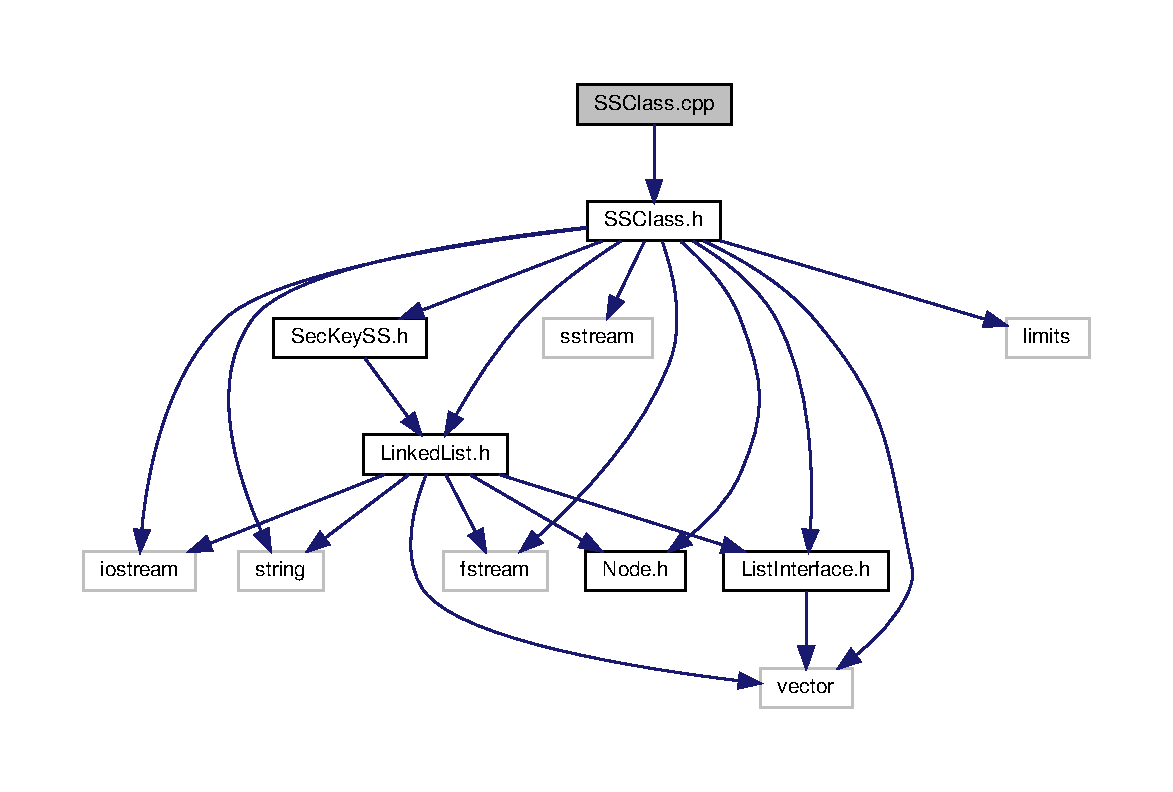
\includegraphics[width=350pt]{SSClass_8cpp__incl}
\end{center}
\end{figure}

\hypertarget{SSClass_8cpp_source}{}\section{S\+S\+Class.\+cpp}

\begin{DoxyCode}
00001 
00002 \textcolor{preprocessor}{#include "\hyperlink{SSClass_8h}{SSClass.h}"}
00003 
00004 
00005 \textcolor{comment}{/*---------------------------------------------------------------------------}
00006 \textcolor{comment}{    Opens file}
00007 \textcolor{comment}{    Preconditions:   File needs to be created}
00008 \textcolor{comment}{    Postconditions:  None}
00009 \textcolor{comment}{*/}
\Hypertarget{SSClass_8cpp_source_l00010}\hyperlink{classSSClass_a92e012441608ea36f3013fb3cbea9da8}{00010} \textcolor{keywordtype}{bool} \hyperlink{classSSClass_a92e012441608ea36f3013fb3cbea9da8}{SSClass::openFile}(\textcolor{keywordtype}{string} input) \{ \textcolor{comment}{//input is a file name}
00011     indexFile.open(input);
00012     nextEmpty = -1;
00013     \textcolor{keywordflow}{return} (indexFile.is\_open());
00014 
00015 \}
00016 
00017 \textcolor{comment}{/*}
00018 \textcolor{comment}{bool SSClass::createIndexFile() \{}
00019 \textcolor{comment}{    indexFile.open("index.txt");}
00020 \textcolor{comment}{    return indexFile.is\_open();}
00021 \textcolor{comment}{\}}
00022 \textcolor{comment}{*/}
00023 \textcolor{comment}{/*---------------------------------------------------------------------------}
00024 \textcolor{comment}{    Creates block record file}
00025 \textcolor{comment}{    Preconditions:   None}
00026 \textcolor{comment}{    Postconditions:  None}
00027 \textcolor{comment}{*/}
00028 \textcolor{comment}{/*}
00029 \textcolor{comment}{bool SSClass::createBlockRecordFile() \{}
00030 \textcolor{comment}{    blockRecordFile.open("blockRecord.txt");}
00031 \textcolor{comment}{    return blockRecord.is\_open();}
00032 \textcolor{comment}{\}}
00033 \textcolor{comment}{*/}
00034 \textcolor{comment}{/*---------------------------------------------------------------------------}
00035 \textcolor{comment}{    Default constructor}
00036 \textcolor{comment}{    Preconditions:   None}
00037 \textcolor{comment}{    Postconditions:  None}
00038 \textcolor{comment}{*/}
\Hypertarget{SSClass_8cpp_source_l00039}\hyperlink{classSSClass_ab4603d6a236c4fa65f896a1158c0d2ef}{00039} \hyperlink{classSSClass_ab4603d6a236c4fa65f896a1158c0d2ef}{SSClass::SSClass}() \{
00040     numRecords = 0;
00041     \hyperlink{classSSClass_a92e012441608ea36f3013fb3cbea9da8}{openFile}(\textcolor{stringliteral}{"us\_postal\_codes.txt"});
00042 \}
\Hypertarget{SSClass_8cpp_source_l00043}\hyperlink{classSSClass_a5801614847b5403b1a5899150acd3b5c}{00043} \hyperlink{classSSClass_ab4603d6a236c4fa65f896a1158c0d2ef}{SSClass::SSClass}(\textcolor{keyword}{const} \hyperlink{classSSClass}{SSClass}& ss) \{
00044     numLinesIndex = ss.numLinesIndex;
00045     numRecords = ss.numRecords;
00046     nextEmpty = ss.nextEmpty;
00047     secKeyZip = ss.secKeyZip;
00048     secKeyPlace= ss.secKeyPlace;
00049     secKeyState = ss.secKeyState;
00050     secKeyCounty = ss.secKeyCounty;
00051     secKeyLat = ss.secKeyLat;
00052     secKeyLon = ss.secKeyLon;
00053     \hyperlink{classSSClass_a92e012441608ea36f3013fb3cbea9da8}{openFile}(\textcolor{stringliteral}{"us\_postal\_codes.txt"});
00054 \}
\Hypertarget{SSClass_8cpp_source_l00055}\hyperlink{classSSClass_a6e5abb04de9b90e34cc6422069ff5729}{00055} \hyperlink{classSSClass_a6e5abb04de9b90e34cc6422069ff5729}{SSClass::~SSClass}()\{
00056     secKeyZip.\hyperlink{classLinkedList_a7d1d9cf83eef67b6c4d700a3cc5970e1}{clear}();
00057     secKeyPlace.\hyperlink{classLinkedList_a7d1d9cf83eef67b6c4d700a3cc5970e1}{clear}();
00058     secKeyState.\hyperlink{classLinkedList_a7d1d9cf83eef67b6c4d700a3cc5970e1}{clear}();
00059     secKeyCounty.\hyperlink{classLinkedList_a7d1d9cf83eef67b6c4d700a3cc5970e1}{clear}();
00060     secKeyLat.\hyperlink{classLinkedList_a7d1d9cf83eef67b6c4d700a3cc5970e1}{clear}();
00061     secKeyLon.\hyperlink{classLinkedList_a7d1d9cf83eef67b6c4d700a3cc5970e1}{clear}();
00062     indexFile.close();
00063     \textcolor{comment}{//blockRecord.close();}
00064 \}
00065 
\Hypertarget{SSClass_8cpp_source_l00070}\hyperlink{classSSClass_a45c5585c784bf7c4f823f66426664aea}{00070} \textcolor{keywordtype}{void} \hyperlink{classSSClass_a45c5585c784bf7c4f823f66426664aea}{SSClass::insert}(\textcolor{keywordtype}{string} s) \{
00071     \textcolor{keywordflow}{if} (nextEmpty == -1) \{
00072         goToLine(indexFile, numLinesIndex);
00073         indexFile << \textcolor{stringliteral}{"\(\backslash\)n"} << s;
00074         insertZip(getZip(s), numLinesIndex);
00075         insertPlace(getPlace(s), numLinesIndex);
00076         insertState(getState(s), numLinesIndex);
00077         insertCounty(getCounty(s), numLinesIndex);
00078         insertLat(getLat(s), numLinesIndex);
00079         insertLon(getLon(s), numLinesIndex);
00080         numLinesIndex++;
00081         \textcolor{keywordflow}{return};
00082     \}
00083     goToLine(indexFile, nextEmpty);
00084     \textcolor{comment}{//replace(s, nextEmpty);}
00085     insertZip(getZip(s), nextEmpty);
00086     insertPlace(getPlace(s), nextEmpty);
00087     insertState(getState(s), nextEmpty);
00088     insertCounty(getCounty(s), nextEmpty);
00089     insertLat(getLat(s), nextEmpty);
00090     insertLon(getLon(s), nextEmpty);
00091 \}
00092 
\Hypertarget{SSClass_8cpp_source_l00093}\hyperlink{classSSClass_ab0a8ea1af895df28359b5733bd920ef3}{00093} \textcolor{keywordtype}{string} \hyperlink{classSSClass_ab0a8ea1af895df28359b5733bd920ef3}{SSClass::returnLine}(\textcolor{keywordtype}{int} rrn) \{
00094     \textcolor{keywordtype}{string} returnVal;
00095     goToLine(indexFile, rrn);
00096     getline(indexFile, returnVal);
00097     \textcolor{keywordflow}{return} returnVal;
00098 \}
00099 
00100 
\Hypertarget{SSClass_8cpp_source_l00101}\hyperlink{classSSClass_a9df3598c000a6a5e9ef994d19196e69f}{00101} vector<int> \hyperlink{classSSClass_a9df3598c000a6a5e9ef994d19196e69f}{SSClass::search}(\textcolor{keywordtype}{string} s, \textcolor{keywordtype}{unsigned} fieldNum) \{
00102     \textcolor{keyword}{typedef} \hyperlink{classSecKeySS}{SecKeySS<string>} secCopy;
00103     \textcolor{keywordtype}{int} i;
00104     vector<int> results;
00105     \textcolor{keywordflow}{switch} (fieldNum) \{
00106     \textcolor{keywordflow}{case} 1:
00107     \{
00108         \textcolor{keywordflow}{for} (i = 1; (i < (secKeyZip.\hyperlink{classLinkedList_afc6635f854f48f2f126cf3b60d845220}{getItemCount}() + 1)) && (secKeyZip.
      \hyperlink{classLinkedList_a341bfd7772c9d24d29eb7a7f3936915b}{getEntry}(i).\hyperlink{classSecKeySS_a9fdb8a771250b7aaab556f019b381eab}{getData}() < stoi(s)); i++);
00109         \textcolor{keywordflow}{if} (secKeyZip.\hyperlink{classLinkedList_a341bfd7772c9d24d29eb7a7f3936915b}{getEntry}(i).\hyperlink{classSecKeySS_a9fdb8a771250b7aaab556f019b381eab}{getData}() == stoi(s)) \{
00110             \hyperlink{classLinkedList}{LinkedList<int>} toCopy = \hyperlink{classLinkedList}{LinkedList<int>}(secKeyZip.
      \hyperlink{classLinkedList_a341bfd7772c9d24d29eb7a7f3936915b}{getEntry}(i).\hyperlink{classSecKeySS_abef7c9c03e9bc6b818d599966428fdec}{getDuplicates}());
00111             \textcolor{keywordflow}{for} (\textcolor{keywordtype}{int} j = 1; j < (toCopy.\hyperlink{classLinkedList_afc6635f854f48f2f126cf3b60d845220}{getItemCount}() + 1); j++) \{
00112                 results.push\_back(toCopy.\hyperlink{classLinkedList_a341bfd7772c9d24d29eb7a7f3936915b}{getEntry}(j));
00113             \}
00114         \}
00115     \}
00116     \textcolor{keywordflow}{break};
00117     \textcolor{keywordflow}{case} 2:
00118     \{
00119         \textcolor{keywordflow}{for}(i = 1; (i < (secKeyPlace.\hyperlink{classLinkedList_afc6635f854f48f2f126cf3b60d845220}{getItemCount}() + 1)) && (secKeyPlace.
      \hyperlink{classLinkedList_a341bfd7772c9d24d29eb7a7f3936915b}{getEntry}(i).\hyperlink{classSecKeySS_a9fdb8a771250b7aaab556f019b381eab}{getData}() < s); i++);
00120         \textcolor{keywordflow}{if} ((secKeyPlace.\hyperlink{classLinkedList_a341bfd7772c9d24d29eb7a7f3936915b}{getEntry}(i).\hyperlink{classSecKeySS_a9fdb8a771250b7aaab556f019b381eab}{getData}()) == (s)) \{
00121             \hyperlink{classLinkedList}{LinkedList<string>} toCopy = \hyperlink{classLinkedList}{LinkedList<string>}(secKeyPlace.
      \hyperlink{classLinkedList_a341bfd7772c9d24d29eb7a7f3936915b}{getEntry}(i).\hyperlink{classSecKeySS_abef7c9c03e9bc6b818d599966428fdec}{getDuplicates}());
00122             \textcolor{keywordflow}{for} (\textcolor{keywordtype}{int} j = 1; j < (toCopy.\hyperlink{classLinkedList_afc6635f854f48f2f126cf3b60d845220}{getItemCount}() + 1); j++) \{
00123                 \textcolor{comment}{// stoi toCopy.getEntry returns string}
00124                 results.push\_back(stoi(toCopy.\hyperlink{classLinkedList_a341bfd7772c9d24d29eb7a7f3936915b}{getEntry}(j)));
00125             \}
00126         \}
00127     \}
00128     \textcolor{keywordflow}{break};
00129     \textcolor{keywordflow}{case} 3:
00130     \{
00131         \textcolor{keywordflow}{for} (i = 1; (i < (secKeyState.\hyperlink{classLinkedList_afc6635f854f48f2f126cf3b60d845220}{getItemCount}() + 1)) && (secKeyState.
      \hyperlink{classLinkedList_a341bfd7772c9d24d29eb7a7f3936915b}{getEntry}(i).\hyperlink{classSecKeySS_a9fdb8a771250b7aaab556f019b381eab}{getData}() < s); i++);
00132         \textcolor{keywordflow}{if} ((secKeyState.\hyperlink{classLinkedList_a341bfd7772c9d24d29eb7a7f3936915b}{getEntry}(i).\hyperlink{classSecKeySS_a9fdb8a771250b7aaab556f019b381eab}{getData}()) == (s)) \{
00133             \hyperlink{classLinkedList}{LinkedList<string>} toCopy = \hyperlink{classLinkedList}{LinkedList<string>}(secKeyState.
      \hyperlink{classLinkedList_a341bfd7772c9d24d29eb7a7f3936915b}{getEntry}(i).\hyperlink{classSecKeySS_abef7c9c03e9bc6b818d599966428fdec}{getDuplicates}());
00134             \textcolor{keywordflow}{for} (\textcolor{keywordtype}{int} j = 1; j < (toCopy.\hyperlink{classLinkedList_afc6635f854f48f2f126cf3b60d845220}{getItemCount}() + 1); j++) \{
00135                 \textcolor{comment}{// stoi toCopy.getEntry returns string}
00136                 results.push\_back(stoi(toCopy.\hyperlink{classLinkedList_a341bfd7772c9d24d29eb7a7f3936915b}{getEntry}(j)));
00137             \}
00138         \}
00139     \}
00140     \textcolor{keywordflow}{break};
00141     \textcolor{keywordflow}{case} 4:
00142     \{
00143         \textcolor{keywordflow}{for} (i = 1; (i < (secKeyCounty.\hyperlink{classLinkedList_afc6635f854f48f2f126cf3b60d845220}{getItemCount}() + 1)) && (secKeyCounty.
      \hyperlink{classLinkedList_a341bfd7772c9d24d29eb7a7f3936915b}{getEntry}(i).\hyperlink{classSecKeySS_a9fdb8a771250b7aaab556f019b381eab}{getData}() < s); i++);
00144         \textcolor{keywordflow}{if} ((secKeyCounty.\hyperlink{classLinkedList_a341bfd7772c9d24d29eb7a7f3936915b}{getEntry}(i).\hyperlink{classSecKeySS_a9fdb8a771250b7aaab556f019b381eab}{getData}()) == (s)) \{
00145             \hyperlink{classLinkedList}{LinkedList<string>} toCopy = \hyperlink{classLinkedList}{LinkedList<string>}(secKeyCounty
      .\hyperlink{classLinkedList_a341bfd7772c9d24d29eb7a7f3936915b}{getEntry}(i).\hyperlink{classSecKeySS_abef7c9c03e9bc6b818d599966428fdec}{getDuplicates}());
00146             \textcolor{keywordflow}{for} (\textcolor{keywordtype}{int} j = 1; j < (toCopy.\hyperlink{classLinkedList_afc6635f854f48f2f126cf3b60d845220}{getItemCount}() + 1); j++) \{
00147                 \textcolor{comment}{// stoi toCopy.getEntry returns string}
00148                 results.push\_back(stoi(toCopy.\hyperlink{classLinkedList_a341bfd7772c9d24d29eb7a7f3936915b}{getEntry}(j)));
00149             \}
00150         \}
00151     \}
00152     \textcolor{keywordflow}{break};
00153     \textcolor{keywordflow}{case} 5:
00154     \{
00155         \textcolor{keywordflow}{for} (i = 1; (i < (secKeyLat.\hyperlink{classLinkedList_afc6635f854f48f2f126cf3b60d845220}{getItemCount}() + 1)) && (secKeyLat.
      \hyperlink{classLinkedList_a341bfd7772c9d24d29eb7a7f3936915b}{getEntry}(i).\hyperlink{classSecKeySS_a9fdb8a771250b7aaab556f019b381eab}{getData}() < stoi(s)); i++);
00156         \textcolor{keywordflow}{if} (secKeyLat.\hyperlink{classLinkedList_a341bfd7772c9d24d29eb7a7f3936915b}{getEntry}(i).\hyperlink{classSecKeySS_a9fdb8a771250b7aaab556f019b381eab}{getData}() == \textcolor{keyword}{static\_cast<}\textcolor{keywordtype}{int}\textcolor{keyword}{>}(stod(s))) \{
00157             \hyperlink{classLinkedList}{LinkedList<int>} toCopy = \hyperlink{classLinkedList}{LinkedList<int>}(secKeyLat.
      \hyperlink{classLinkedList_a341bfd7772c9d24d29eb7a7f3936915b}{getEntry}(i).\hyperlink{classSecKeySS_abef7c9c03e9bc6b818d599966428fdec}{getDuplicates}());
00158             \textcolor{keywordflow}{for} (\textcolor{keywordtype}{int} j = 1; j < (toCopy.\hyperlink{classLinkedList_afc6635f854f48f2f126cf3b60d845220}{getItemCount}() + 1); j++) \{
00159                 results.push\_back(toCopy.\hyperlink{classLinkedList_a341bfd7772c9d24d29eb7a7f3936915b}{getEntry}(j));
00160             \}
00161         \}
00162     \}
00163     \textcolor{keywordflow}{break};
00164     \textcolor{keywordflow}{case} 6:
00165     \{
00166         \textcolor{keywordflow}{for} (i = 1; (i < (secKeyLon.\hyperlink{classLinkedList_afc6635f854f48f2f126cf3b60d845220}{getItemCount}() + 1)) && (secKeyLon.
      \hyperlink{classLinkedList_a341bfd7772c9d24d29eb7a7f3936915b}{getEntry}(i).\hyperlink{classSecKeySS_a9fdb8a771250b7aaab556f019b381eab}{getData}() < stoi(s)); i++);
00167         \textcolor{keywordflow}{if} (secKeyLon.\hyperlink{classLinkedList_a341bfd7772c9d24d29eb7a7f3936915b}{getEntry}(i).\hyperlink{classSecKeySS_a9fdb8a771250b7aaab556f019b381eab}{getData}() == \textcolor{keyword}{static\_cast<}\textcolor{keywordtype}{int}\textcolor{keyword}{>}(stod(s))) \{
00168             \hyperlink{classLinkedList}{LinkedList<int>} toCopy = \hyperlink{classLinkedList}{LinkedList<int>}(secKeyLon.
      \hyperlink{classLinkedList_a341bfd7772c9d24d29eb7a7f3936915b}{getEntry}(i).\hyperlink{classSecKeySS_abef7c9c03e9bc6b818d599966428fdec}{getDuplicates}());
00169             \textcolor{keywordflow}{for} (\textcolor{keywordtype}{int} j = 1; j < (toCopy.\hyperlink{classLinkedList_afc6635f854f48f2f126cf3b60d845220}{getItemCount}() + 1); j++) \{
00170                 results.push\_back(toCopy.\hyperlink{classLinkedList_a341bfd7772c9d24d29eb7a7f3936915b}{getEntry}(j));
00171             \}
00172         \}
00173     \}
00174     \textcolor{keywordflow}{break};
00175     \}
00176     \textcolor{keywordflow}{return} results;
00177 \}
00178 
\Hypertarget{SSClass_8cpp_source_l00179}\hyperlink{classSSClass_ad03c99840c2946a2112f5f1942c287f2}{00179} \textcolor{keywordtype}{int} \hyperlink{classSSClass_ad03c99840c2946a2112f5f1942c287f2}{SSClass::directionalSearch}(\textcolor{keywordtype}{string} stateS, \textcolor{keywordtype}{char} direction) \{
00180     direction = toupper(direction);
00181     \textcolor{keywordtype}{int} i = 1;
00182     \textcolor{keywordtype}{int} returnIndex = -1;
00183     \textcolor{keywordtype}{double} highOrLow;
00184     vector<int> state = \hyperlink{classSSClass_a9df3598c000a6a5e9ef994d19196e69f}{search}(stateS, 3);
00185     \textcolor{keywordflow}{switch} (direction) \{
00186     \textcolor{keywordflow}{case} \textcolor{charliteral}{'N'}:
00187     \{
00188         returnIndex = state[0];
00189         highOrLow = stod(getLat(\hyperlink{classSSClass_ab0a8ea1af895df28359b5733bd920ef3}{returnLine}(state[0])));
00190         \textcolor{keywordflow}{for} (i; i < state.size(); i++) \{
00191             \textcolor{keywordflow}{if} (highOrLow < stod(getLat(\hyperlink{classSSClass_ab0a8ea1af895df28359b5733bd920ef3}{returnLine}(state[i])))) \{
00192                 highOrLow = stod(getLat(\hyperlink{classSSClass_ab0a8ea1af895df28359b5733bd920ef3}{returnLine}(state[i])));
00193                 returnIndex = i;
00194             \}
00195 
00196         \}
00197     \}
00198     \textcolor{keywordflow}{break};
00199     \textcolor{keywordflow}{case} \textcolor{charliteral}{'E'}:
00200     \{
00201         returnIndex = state[0];
00202         highOrLow = stod(getLon(\hyperlink{classSSClass_ab0a8ea1af895df28359b5733bd920ef3}{returnLine}(state[0])));
00203         \textcolor{keywordflow}{for} (i; i < state.size(); i++) \{
00204             \textcolor{keywordflow}{if} (highOrLow < stod(getLon(\hyperlink{classSSClass_ab0a8ea1af895df28359b5733bd920ef3}{returnLine}(state[i])))) \{
00205                 highOrLow = stod(getLon(\hyperlink{classSSClass_ab0a8ea1af895df28359b5733bd920ef3}{returnLine}(state[i])));
00206                 returnIndex = i;
00207             \}
00208         \}
00209         
00210     \}
00211     \textcolor{keywordflow}{break};
00212     \textcolor{keywordflow}{case} \textcolor{charliteral}{'S'}:
00213     \{
00214         returnIndex = state[0];
00215         highOrLow = stod(getLat(\hyperlink{classSSClass_ab0a8ea1af895df28359b5733bd920ef3}{returnLine}(state[0])));
00216         \textcolor{keywordflow}{for} (i; i < state.size(); i++) \{
00217             \textcolor{keywordflow}{if} (highOrLow > stod(getLat(\hyperlink{classSSClass_ab0a8ea1af895df28359b5733bd920ef3}{returnLine}(state[i])))) \{
00218                 highOrLow = stod(getLat(\hyperlink{classSSClass_ab0a8ea1af895df28359b5733bd920ef3}{returnLine}(state[i])));
00219                 returnIndex = i;
00220             \}
00221         \}
00222         \textcolor{keywordflow}{break};
00223     \}
00224     \textcolor{keywordflow}{case} \textcolor{charliteral}{'W'}:
00225     \{
00226         returnIndex = state[0];
00227         highOrLow = stod(getLon(\hyperlink{classSSClass_ab0a8ea1af895df28359b5733bd920ef3}{returnLine}(state[0])));
00228         \textcolor{keywordflow}{for} (i; i < state.size(); i++) \{
00229             \textcolor{keywordflow}{if} (highOrLow > stod(getLon(\hyperlink{classSSClass_ab0a8ea1af895df28359b5733bd920ef3}{returnLine}(state[i])))) \{
00230                 highOrLow = stod(getLon(\hyperlink{classSSClass_ab0a8ea1af895df28359b5733bd920ef3}{returnLine}(state[i])));
00231                 returnIndex = i;
00232             \}
00233         \}
00234 
00235     \}
00236     \textcolor{keywordflow}{break};
00237     \}
00238     \textcolor{keywordflow}{return} returnIndex;
00239 
00240 \}
00241 
00242 \textcolor{comment}{//get value at index in getEntry(index)         insert is insert(index)   }
00243 \textcolor{keywordtype}{void} SSClass::insertZip(\textcolor{keywordtype}{string} st, \textcolor{keywordtype}{int} rrn) \{                \textcolor{comment}{//no sec key matching -> create new one....   
       match found -> insert at index 1}
00244     \textcolor{keywordtype}{int} index;
00245     \textcolor{keywordtype}{int} s = stoi(st);
00246     \hyperlink{classSecKeySS}{SecKeySS<int>} secCopy;
00247     \hyperlink{classLinkedList}{LinkedList<int>} copyDup;
00248         \textcolor{keywordtype}{int} i;
00249     \textcolor{keywordflow}{for} (i = 1; (i < (secKeyZip.\hyperlink{classLinkedList_afc6635f854f48f2f126cf3b60d845220}{getItemCount}() + 1)) && (secKeyZip.
      \hyperlink{classLinkedList_a341bfd7772c9d24d29eb7a7f3936915b}{getEntry}(i).\hyperlink{classSecKeySS_a9fdb8a771250b7aaab556f019b381eab}{getData}() < s); i++);
00250     \textcolor{keywordflow}{if} (secKeyZip.\hyperlink{classLinkedList_a341bfd7772c9d24d29eb7a7f3936915b}{getEntry}(i).\hyperlink{classSecKeySS_a9fdb8a771250b7aaab556f019b381eab}{getData}() == s) \{
00251         secCopy = secKeyZip.\hyperlink{classLinkedList_a341bfd7772c9d24d29eb7a7f3936915b}{getEntry}(i);
00252         copyDup = \hyperlink{classLinkedList}{LinkedList<int>}(secCopy.\hyperlink{classSecKeySS_abef7c9c03e9bc6b818d599966428fdec}{getDuplicates}());
00253         copyDup.\hyperlink{classLinkedList_ae8a19375505e87e2e4fc0e9b5afe4d4d}{insert}(1, rrn);
00254         secCopy.\hyperlink{classSecKeySS_a95fdde8fc0b590359692784d15481dd4}{setDuplicates}(copyDup);
00255         secKeyZip.\hyperlink{classLinkedList_a3035f880c50e7d8f68e67c093d4607ca}{replace}(i, secCopy);
00256         \textcolor{keywordflow}{return};
00257     \}
00258     copyDup.\hyperlink{classLinkedList_ae8a19375505e87e2e4fc0e9b5afe4d4d}{insert}(1, rrn);
00259     secCopy.\hyperlink{classSecKeySS_a95fdde8fc0b590359692784d15481dd4}{setDuplicates}(copyDup);
00260     secCopy.\hyperlink{classSecKeySS_ae893fbaf619bf61f73f1585ae5686609}{setData}(s);
00261     secKeyZip.\hyperlink{classLinkedList_ae8a19375505e87e2e4fc0e9b5afe4d4d}{insert}(i, secCopy);
00262 
00263 \}
00264 
00265 \textcolor{keywordtype}{void} SSClass::insertPlace(\textcolor{keywordtype}{string} s, \textcolor{keywordtype}{int} rrn) \{
00266     \textcolor{keywordtype}{int} index;
00267     \hyperlink{classSecKeySS}{SecKeySS<string>} secCopy;
00268     \hyperlink{classLinkedList}{LinkedList<string>} copyDup;
00269         \textcolor{keywordtype}{int} i;
00270     \textcolor{keywordflow}{for} (i = 1; (i < (secKeyPlace.\hyperlink{classLinkedList_afc6635f854f48f2f126cf3b60d845220}{getItemCount}() + 1)) && (secKeyPlace.
      \hyperlink{classLinkedList_a341bfd7772c9d24d29eb7a7f3936915b}{getEntry}(i).\hyperlink{classSecKeySS_a9fdb8a771250b7aaab556f019b381eab}{getData}() < s); i++);
00271     \textcolor{keywordflow}{if} (secKeyPlace.\hyperlink{classLinkedList_a341bfd7772c9d24d29eb7a7f3936915b}{getEntry}(i).\hyperlink{classSecKeySS_a9fdb8a771250b7aaab556f019b381eab}{getData}() == s) \{
00272         secCopy = secKeyPlace.\hyperlink{classLinkedList_a341bfd7772c9d24d29eb7a7f3936915b}{getEntry}(i);
00273         copyDup = \hyperlink{classLinkedList}{LinkedList<string>}(secCopy.\hyperlink{classSecKeySS_abef7c9c03e9bc6b818d599966428fdec}{getDuplicates}());
00274         copyDup.\hyperlink{classLinkedList_ae8a19375505e87e2e4fc0e9b5afe4d4d}{insert}(1, to\_string(rrn));
00275         secCopy.\hyperlink{classSecKeySS_a95fdde8fc0b590359692784d15481dd4}{setDuplicates}(copyDup);
00276         secKeyPlace.\hyperlink{classLinkedList_a3035f880c50e7d8f68e67c093d4607ca}{replace}(i, secCopy);
00277         \textcolor{keywordflow}{return};
00278     \}
00279     copyDup.\hyperlink{classLinkedList_ae8a19375505e87e2e4fc0e9b5afe4d4d}{insert}(1, to\_string(rrn));
00280     secCopy.\hyperlink{classSecKeySS_a95fdde8fc0b590359692784d15481dd4}{setDuplicates}(copyDup);
00281     secCopy.\hyperlink{classSecKeySS_ae893fbaf619bf61f73f1585ae5686609}{setData}(getPlace(s));
00282     secKeyPlace.\hyperlink{classLinkedList_ae8a19375505e87e2e4fc0e9b5afe4d4d}{insert}(i, secCopy);
00283 \}
00284 
00285 \textcolor{keywordtype}{void} SSClass::insertState(\textcolor{keywordtype}{string} s, \textcolor{keywordtype}{int} rrn) \{
00286     \textcolor{keywordtype}{int} index;
00287     \hyperlink{classSecKeySS}{SecKeySS<string>} secCopy;
00288     \hyperlink{classLinkedList}{LinkedList<string>} copyDup;
00289         \textcolor{keywordtype}{int} i;
00290     \textcolor{keywordflow}{for} (i = 1; (i < (secKeyState.\hyperlink{classLinkedList_afc6635f854f48f2f126cf3b60d845220}{getItemCount}() + 1)) && (secKeyState.
      \hyperlink{classLinkedList_a341bfd7772c9d24d29eb7a7f3936915b}{getEntry}(i).\hyperlink{classSecKeySS_a9fdb8a771250b7aaab556f019b381eab}{getData}() < s); i++);
00291     \textcolor{keywordflow}{if} (secKeyState.\hyperlink{classLinkedList_a341bfd7772c9d24d29eb7a7f3936915b}{getEntry}(i).\hyperlink{classSecKeySS_a9fdb8a771250b7aaab556f019b381eab}{getData}() == s) \{
00292         secCopy = secKeyState.\hyperlink{classLinkedList_a341bfd7772c9d24d29eb7a7f3936915b}{getEntry}(i);
00293         copyDup = \hyperlink{classLinkedList}{LinkedList<string>}(secCopy.\hyperlink{classSecKeySS_abef7c9c03e9bc6b818d599966428fdec}{getDuplicates}());
00294         copyDup.\hyperlink{classLinkedList_ae8a19375505e87e2e4fc0e9b5afe4d4d}{insert}(1, to\_string(rrn));
00295         secCopy.\hyperlink{classSecKeySS_a95fdde8fc0b590359692784d15481dd4}{setDuplicates}(copyDup);
00296         secKeyState.\hyperlink{classLinkedList_a3035f880c50e7d8f68e67c093d4607ca}{replace}(i, secCopy);
00297         \textcolor{keywordflow}{return};
00298     \}
00299     copyDup.\hyperlink{classLinkedList_ae8a19375505e87e2e4fc0e9b5afe4d4d}{insert}(1, to\_string(rrn));
00300     secCopy.\hyperlink{classSecKeySS_a95fdde8fc0b590359692784d15481dd4}{setDuplicates}(copyDup);
00301     secCopy.\hyperlink{classSecKeySS_ae893fbaf619bf61f73f1585ae5686609}{setData}(getState(s));
00302     secKeyState.\hyperlink{classLinkedList_ae8a19375505e87e2e4fc0e9b5afe4d4d}{insert}(i, secCopy);
00303 \}
00304 
00305 \textcolor{keywordtype}{void} SSClass::insertCounty(\textcolor{keywordtype}{string} s, \textcolor{keywordtype}{int} rrn) \{
00306     \textcolor{keywordtype}{int} index;
00307     \hyperlink{classSecKeySS}{SecKeySS<string>} secCopy;
00308     \hyperlink{classLinkedList}{LinkedList<string>} copyDup;
00309         \textcolor{keywordtype}{int} i;
00310     \textcolor{keywordflow}{for} (i = 1; (i < (secKeyCounty.\hyperlink{classLinkedList_afc6635f854f48f2f126cf3b60d845220}{getItemCount}() + 1)) && (secKeyCounty.
      \hyperlink{classLinkedList_a341bfd7772c9d24d29eb7a7f3936915b}{getEntry}(i).\hyperlink{classSecKeySS_a9fdb8a771250b7aaab556f019b381eab}{getData}() < s); i++);
00311     \textcolor{keywordflow}{if} (secKeyCounty.\hyperlink{classLinkedList_a341bfd7772c9d24d29eb7a7f3936915b}{getEntry}(i).\hyperlink{classSecKeySS_a9fdb8a771250b7aaab556f019b381eab}{getData}() == s) \{
00312         secCopy = secKeyCounty.\hyperlink{classLinkedList_a341bfd7772c9d24d29eb7a7f3936915b}{getEntry}(i);
00313         copyDup = \hyperlink{classLinkedList}{LinkedList<string>}(secCopy.\hyperlink{classSecKeySS_abef7c9c03e9bc6b818d599966428fdec}{getDuplicates}());
00314         copyDup.\hyperlink{classLinkedList_ae8a19375505e87e2e4fc0e9b5afe4d4d}{insert}(1, to\_string(rrn));
00315         secCopy.\hyperlink{classSecKeySS_a95fdde8fc0b590359692784d15481dd4}{setDuplicates}(copyDup);
00316         secKeyCounty.\hyperlink{classLinkedList_a3035f880c50e7d8f68e67c093d4607ca}{replace}(i, secCopy);
00317         \textcolor{keywordflow}{return};
00318     \}
00319     copyDup.\hyperlink{classLinkedList_ae8a19375505e87e2e4fc0e9b5afe4d4d}{insert}(1, to\_string(rrn));
00320     secCopy.\hyperlink{classSecKeySS_a95fdde8fc0b590359692784d15481dd4}{setDuplicates}(copyDup);
00321     secCopy.\hyperlink{classSecKeySS_ae893fbaf619bf61f73f1585ae5686609}{setData}(getCounty(s));
00322     secKeyCounty.\hyperlink{classLinkedList_ae8a19375505e87e2e4fc0e9b5afe4d4d}{insert}(i, secCopy);
00323 \}
00324 
00325 \textcolor{keywordtype}{void} SSClass::insertLat(\textcolor{keywordtype}{string} st, \textcolor{keywordtype}{int} rrn) \{
00326     \textcolor{keywordtype}{int} index;
00327     \textcolor{keywordtype}{int} s = \textcolor{keyword}{static\_cast<}\textcolor{keywordtype}{int}\textcolor{keyword}{>}(stod(st));
00328     \hyperlink{classSecKeySS}{SecKeySS<int>} secCopy;
00329     \hyperlink{classLinkedList}{LinkedList<int>} copyDup;
00330         \textcolor{keywordtype}{int} i;
00331     \textcolor{keywordflow}{for} (i = 1; (i < (secKeyLat.\hyperlink{classLinkedList_afc6635f854f48f2f126cf3b60d845220}{getItemCount}() + 1)) && (secKeyLat.
      \hyperlink{classLinkedList_a341bfd7772c9d24d29eb7a7f3936915b}{getEntry}(i).\hyperlink{classSecKeySS_a9fdb8a771250b7aaab556f019b381eab}{getData}() < s); i++);
00332     \textcolor{keywordflow}{if} (secKeyLat.\hyperlink{classLinkedList_a341bfd7772c9d24d29eb7a7f3936915b}{getEntry}(i).\hyperlink{classSecKeySS_a9fdb8a771250b7aaab556f019b381eab}{getData}() == s) \{
00333         secCopy = secKeyLat.\hyperlink{classLinkedList_a341bfd7772c9d24d29eb7a7f3936915b}{getEntry}(i);
00334         copyDup = \hyperlink{classLinkedList}{LinkedList<int>}(secCopy.\hyperlink{classSecKeySS_abef7c9c03e9bc6b818d599966428fdec}{getDuplicates}());
00335         copyDup.\hyperlink{classLinkedList_ae8a19375505e87e2e4fc0e9b5afe4d4d}{insert}(1, rrn);
00336         secCopy.\hyperlink{classSecKeySS_a95fdde8fc0b590359692784d15481dd4}{setDuplicates}(copyDup);
00337         secKeyLat.\hyperlink{classLinkedList_a3035f880c50e7d8f68e67c093d4607ca}{replace}(i, secCopy);
00338         \textcolor{keywordflow}{return};
00339     \}
00340     copyDup.\hyperlink{classLinkedList_ae8a19375505e87e2e4fc0e9b5afe4d4d}{insert}(1, rrn);
00341     secCopy.\hyperlink{classSecKeySS_a95fdde8fc0b590359692784d15481dd4}{setDuplicates}(copyDup);
00342     secCopy.\hyperlink{classSecKeySS_ae893fbaf619bf61f73f1585ae5686609}{setData}(static\_cast<int>(stod(st)));
00343     secKeyLat.\hyperlink{classLinkedList_ae8a19375505e87e2e4fc0e9b5afe4d4d}{insert}(i, secCopy);
00344 \}
00345 
00346 \textcolor{keywordtype}{void} SSClass::insertLon(\textcolor{keywordtype}{string} st, \textcolor{keywordtype}{int} rrn) \{
00347     \textcolor{keywordtype}{int} index;
00348     \textcolor{keywordtype}{int} s = \textcolor{keyword}{static\_cast<}\textcolor{keywordtype}{int}\textcolor{keyword}{>}(stod(st));
00349     \hyperlink{classSecKeySS}{SecKeySS<int>} secCopy;
00350     \hyperlink{classLinkedList}{LinkedList<int>} copyDup;
00351         \textcolor{keywordtype}{int} i;
00352     \textcolor{keywordflow}{for} (i = 1; (i < (secKeyLon.\hyperlink{classLinkedList_afc6635f854f48f2f126cf3b60d845220}{getItemCount}() + 1)) && (secKeyLon.
      \hyperlink{classLinkedList_a341bfd7772c9d24d29eb7a7f3936915b}{getEntry}(i).\hyperlink{classSecKeySS_a9fdb8a771250b7aaab556f019b381eab}{getData}() < s); i++);
00353     \textcolor{keywordflow}{if} (secKeyLon.\hyperlink{classLinkedList_a341bfd7772c9d24d29eb7a7f3936915b}{getEntry}(i).\hyperlink{classSecKeySS_a9fdb8a771250b7aaab556f019b381eab}{getData}() == s) \{
00354         secCopy = secKeyLon.\hyperlink{classLinkedList_a341bfd7772c9d24d29eb7a7f3936915b}{getEntry}(i);
00355         copyDup = \hyperlink{classLinkedList}{LinkedList<int>}(secCopy.\hyperlink{classSecKeySS_abef7c9c03e9bc6b818d599966428fdec}{getDuplicates}());
00356         copyDup.\hyperlink{classLinkedList_ae8a19375505e87e2e4fc0e9b5afe4d4d}{insert}(1, rrn);
00357         secCopy.\hyperlink{classSecKeySS_a95fdde8fc0b590359692784d15481dd4}{setDuplicates}(copyDup);
00358         secKeyLon.\hyperlink{classLinkedList_a3035f880c50e7d8f68e67c093d4607ca}{replace}(i, secCopy);
00359         \textcolor{keywordflow}{return};
00360     \}
00361     copyDup.\hyperlink{classLinkedList_ae8a19375505e87e2e4fc0e9b5afe4d4d}{insert}(1, rrn);
00362     secCopy.\hyperlink{classSecKeySS_a95fdde8fc0b590359692784d15481dd4}{setDuplicates}(copyDup);
00363     secCopy.\hyperlink{classSecKeySS_ae893fbaf619bf61f73f1585ae5686609}{setData}(static\_cast<int>(stod(st)));
00364     secKeyLon.\hyperlink{classLinkedList_ae8a19375505e87e2e4fc0e9b5afe4d4d}{insert}(i, secCopy);
00365 \}
00366 
00367 \textcolor{keywordtype}{void} SSClass::goToLine(fstream& file, \textcolor{keywordtype}{unsigned} num) \{
00368     goToData(file); \textcolor{comment}{//beginning of our data file}
00369     \textcolor{keywordflow}{for} (\textcolor{keywordtype}{int} i = 0; i < num - 1; ++i) \{
00370         file.ignore(1000, \textcolor{charliteral}{'\(\backslash\)n'}); \textcolor{comment}{//ignore one line}
00371     \}
00372     \textcolor{comment}{//return file;}
00373 \}
00374 
00375 \textcolor{keywordtype}{void} SSClass::goToData(fstream& file) \{ \textcolor{comment}{//puts cursor at the beginning of the data portion of the txt file}
00376     file.seekg(ios::beg);
00377     \textcolor{keywordtype}{string} in;
00378     getline(file, in);
00379     \textcolor{keywordflow}{while} (in != \textcolor{stringliteral}{"ENDOFHDR"})
00380         getline(file, in);
00381 \}
00382 
00383 \textcolor{keywordtype}{string} SSClass::getZip(\textcolor{keywordtype}{string} s) \{ \textcolor{comment}{//use stoi(getzip(s)); to return int value}
00384     \textcolor{keywordtype}{string} returnValue;
00385     \textcolor{keywordflow}{for} (\textcolor{keywordtype}{int} i = 0; i < \hyperlink{SSClass_8h_afed733ffdf6aafbaf75b52ea1999b6b4}{ZIPSIZE}; i++)
00386         returnValue[i] = s[\hyperlink{SSClass_8h_a23160a846653bd4df3c5b10c77d23073}{ZIPOFFSET} + i];
00387     \textcolor{keywordflow}{return} returnValue;
00388 \}
00389 
00390 \textcolor{keywordtype}{string} SSClass::getPlace(\textcolor{keywordtype}{string} s) \{
00391     \textcolor{keywordtype}{string} returnvalue;
00392     \textcolor{keywordflow}{for} (\textcolor{keywordtype}{int} i = 0; i < \hyperlink{SSClass_8h_a6802669f0c794331636a12aad9da53f5}{PLACESIZE}; i++)
00393         returnvalue[i] = s[\hyperlink{SSClass_8h_af8f8ce23c8243455601f7d14ac1e1f0b}{PLACEOFFSET} + i];
00394     \textcolor{keywordflow}{return} returnvalue;
00395 \}
00396 
00397 \textcolor{keywordtype}{string} SSClass::getState(\textcolor{keywordtype}{string} s) \{
00398     \textcolor{keywordtype}{string} returnvalue;
00399     \textcolor{keywordflow}{for} (\textcolor{keywordtype}{int} i = 0; i < \hyperlink{SSClass_8h_afca7ce02d5a6576fdfbd5e9ec81907d9}{STATESIZE}; i++)
00400         returnvalue[i] = s[\hyperlink{SSClass_8h_a5b27069b5f4f6134864692af92c6a10e}{STATEOFFSET} + i];
00401     \textcolor{keywordflow}{return} returnvalue;
00402 \}
00403 
00404 \textcolor{keywordtype}{string} SSClass::getCounty(\textcolor{keywordtype}{string} s) \{
00405     \textcolor{keywordtype}{string} returnvalue;
00406     \textcolor{keywordflow}{for} (\textcolor{keywordtype}{int} i = 0; i < \hyperlink{SSClass_8h_a5abe6ba10e2e2da36a217ddc89de08ca}{COUNTYSIZE}; i++)
00407         returnvalue[i] = s[\hyperlink{SSClass_8h_a1ef0c56bf76a1106c7a04816609297b6}{COUNTYOFFSET} + i];
00408     \textcolor{keywordflow}{return} returnvalue;
00409 \}
00410 
00411 \textcolor{keywordtype}{string} SSClass::getLat(\textcolor{keywordtype}{string} s) \{ \textcolor{comment}{//use stod(getlat(s)); to return double value}
00412     \textcolor{keywordtype}{string} returnvalue;
00413     \textcolor{keywordflow}{for} (\textcolor{keywordtype}{int} i = 0; i < \hyperlink{SSClass_8h_a68fc5e9dd6f56a07f44be183f6e4838b}{LATSIZE}; i++)
00414         returnvalue[i] = s[\hyperlink{SSClass_8h_a008e15601aa41491b6e9093364fbe38a}{LATOFFSET} + i];
00415     \textcolor{keywordflow}{return} returnvalue;
00416 \}
00417 
00418 \textcolor{keywordtype}{string} SSClass::getLon(\textcolor{keywordtype}{string} s) \{ \textcolor{comment}{//use stod(getLon(s)); to return double value}
00419     \textcolor{keywordtype}{string} returnValue;
00420     \textcolor{keywordflow}{for} (\textcolor{keywordtype}{int} i = 0; i < \hyperlink{SSClass_8h_a6f928b3e03e80473ea43f148bdb39156}{LONSIZE}; i++)
00421         returnValue[i] = s[\hyperlink{SSClass_8h_a6e916bbc2eb39605cceaee1adc47c3e3}{LONOFFSET} + i];
00422     \textcolor{keywordflow}{return} returnValue;
00423 \}
00424 
00425 \textcolor{keywordtype}{string} SSClass::createUnusedLine(\textcolor{keywordtype}{int} next) \{ \textcolor{comment}{//pass in the integer value of the next empty line}
00426     \textcolor{keywordtype}{string} unusedLine = to\_string(next);
00427     \textcolor{keywordtype}{int} i;
00428     \textcolor{keywordflow}{for} (i = unusedLine.size(); i < \hyperlink{SSClass_8h_ab9a6169c3849700398c71a392857cb9c}{CHARINLINE}; i++) \{
00429         unusedLine += \textcolor{stringliteral}{" "};
00430     \}
00431     \textcolor{keywordflow}{return} unusedLine;
00432 \}
00433 
00434 \textcolor{comment}{/*}
00435 \textcolor{comment}{bool SSClass::replace(string s, int line) \{ // To be able to replace a line in a text file, you have to
       write everything to a new file, with the updated line, then delete the previous file }
00436 \textcolor{comment}{    goToLine(indexFile, line);              // and rename the temperary file}
00437 \textcolor{comment}{    string strReplace;}
00438 \textcolor{comment}{    getline(indexFile, strReplace);}
00439 \textcolor{comment}{    string strNew = s;}
00440 \textcolor{comment}{    ofstream fileout("temp\_file.txt"); //Temporary file}
00441 \textcolor{comment}{    if (!fileout)}
00442 \textcolor{comment}{        return false;}
00443 \textcolor{comment}{}
00444 \textcolor{comment}{    string strTemp;}
00445 \textcolor{comment}{    indexFile.seekg(ios::beg);}
00446 \textcolor{comment}{    while (strTemp = indexFile.getline())}
00447 \textcolor{comment}{    \{}
00448 \textcolor{comment}{        if (strTemp == strReplace) \{}
00449 \textcolor{comment}{            strTemp = strNew;}
00450 \textcolor{comment}{        \}}
00451 \textcolor{comment}{        fileout << "\(\backslash\)n";}
00452 \textcolor{comment}{        for (int i = 0; i < ZIPSIZE; i++) \{ //use this for zip since there may be leading whitespace}
00453 \textcolor{comment}{            fileout << strTemp[i];}
00454 \textcolor{comment}{            strTemp[i] = ' ';}
00455 \textcolor{comment}{        \}}
00456 \textcolor{comment}{        fileout << strTemp;}
00457 \textcolor{comment}{    \}}
00458 \textcolor{comment}{    remove(indexFile);}
00459 \textcolor{comment}{    rename("temp\_file.txt", "us\_postal\_codes.txt");}
00460 \textcolor{comment}{    close(fileout);}
00461 \textcolor{comment}{    openFile("us\_postal\_codes.txt");}
00462 \textcolor{comment}{    return true;}
00463 \textcolor{comment}{\}}
00464 \textcolor{comment}{\}}
00465 \textcolor{comment}{*/}
00466 
00467 \textcolor{keywordtype}{void} SSClass::populate() \{
00468     goToData(indexFile);
00469     \textcolor{keywordtype}{string} line;
00470     \textcolor{keywordflow}{while} (!indexFile.eof()) \{
00471         getline(indexFile, line);
00472         \hyperlink{classSSClass_a45c5585c784bf7c4f823f66426664aea}{insert}(line);
00473     \}
00474 \}
\end{DoxyCode}

\hypertarget{SSClass_8h}{}\section{S\+S\+Class.\+h File Reference}
\label{SSClass_8h}\index{S\+S\+Class.\+h@{S\+S\+Class.\+h}}
{\ttfamily \#include $<$iostream$>$}\newline
{\ttfamily \#include $<$string$>$}\newline
{\ttfamily \#include $<$vector$>$}\newline
{\ttfamily \#include $<$fstream$>$}\newline
{\ttfamily \#include $<$sstream$>$}\newline
{\ttfamily \#include \char`\"{}Linked\+List.\+h\char`\"{}}\newline
{\ttfamily \#include \char`\"{}Node.\+h\char`\"{}}\newline
{\ttfamily \#include \char`\"{}Sec\+Key\+S\+S.\+h\char`\"{}}\newline
{\ttfamily \#include \char`\"{}List\+Interface.\+h\char`\"{}}\newline
{\ttfamily \#include $<$limits$>$}\newline
Include dependency graph for S\+S\+Class.\+h\+:\nopagebreak
\begin{figure}[H]
\begin{center}
\leavevmode
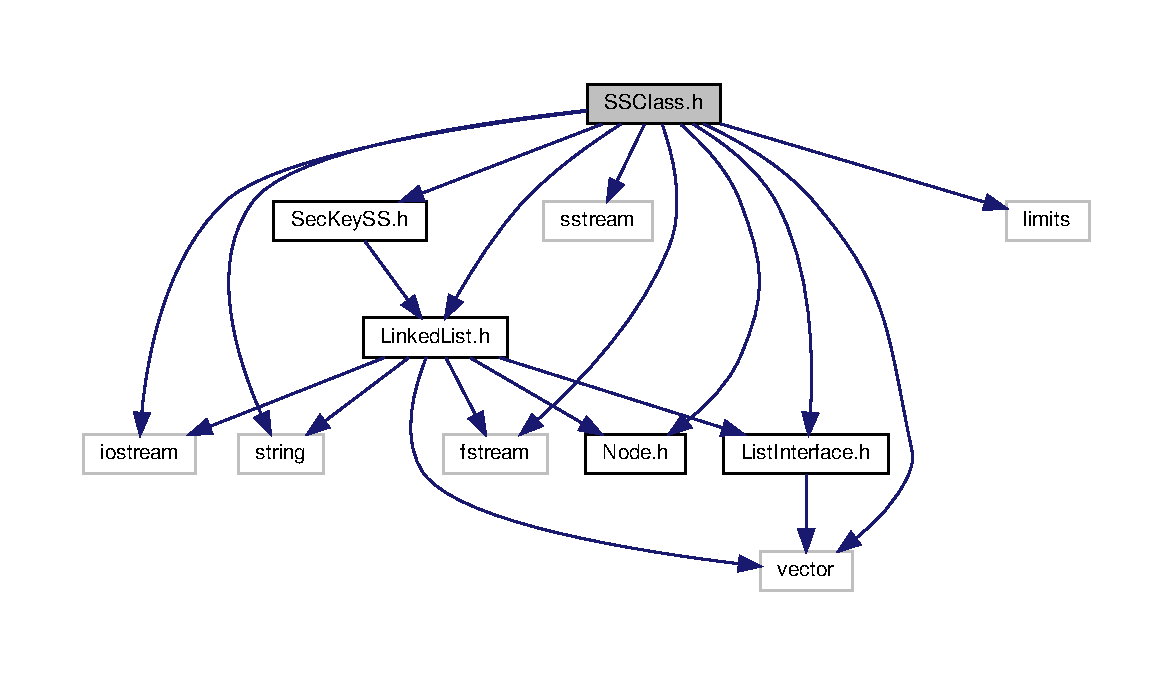
\includegraphics[width=350pt]{SSClass_8h__incl}
\end{center}
\end{figure}
This graph shows which files directly or indirectly include this file\+:\nopagebreak
\begin{figure}[H]
\begin{center}
\leavevmode
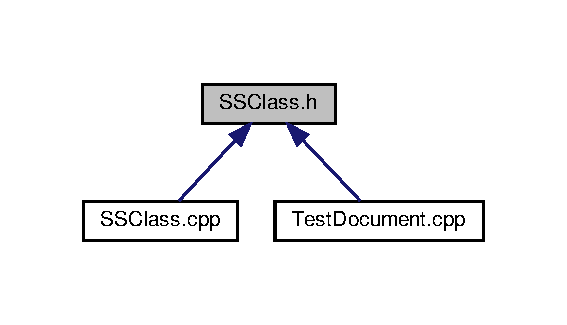
\includegraphics[width=272pt]{SSClass_8h__dep__incl}
\end{center}
\end{figure}
\subsection*{Classes}
\begin{DoxyCompactItemize}
\item 
class \hyperlink{classSSClass}{S\+S\+Class}
\begin{DoxyCompactList}\small\item\em \hyperlink{classLinkedList}{Linked\+List} integration for blocks, records, and fields. \end{DoxyCompactList}\end{DoxyCompactItemize}
\subsection*{Variables}
\begin{DoxyCompactItemize}
\item 
const int \hyperlink{SSClass_8h_ad0b49971b6f96c3d0772461b5de08c1a}{N\+U\+M\+S\+E\+C\+K\+E\+YS} = 6
\begin{DoxyCompactList}\small\item\em N\+U\+M\+S\+E\+C\+K\+E\+YS The numebr of section keys. \end{DoxyCompactList}\item 
const int \hyperlink{SSClass_8h_afed733ffdf6aafbaf75b52ea1999b6b4}{Z\+I\+P\+S\+I\+ZE} = 6
\begin{DoxyCompactList}\small\item\em Z\+I\+P\+S\+I\+ZE The size of the zip code. \end{DoxyCompactList}\item 
const int \hyperlink{SSClass_8h_a6802669f0c794331636a12aad9da53f5}{P\+L\+A\+C\+E\+S\+I\+ZE} = 31
\begin{DoxyCompactList}\small\item\em P\+L\+A\+C\+E\+S\+I\+ZE The size of the place (city) \end{DoxyCompactList}\item 
const int \hyperlink{SSClass_8h_afca7ce02d5a6576fdfbd5e9ec81907d9}{S\+T\+A\+T\+E\+S\+I\+ZE} = 2
\begin{DoxyCompactList}\small\item\em S\+T\+A\+T\+E\+S\+I\+ZE The size of the sate letters. \end{DoxyCompactList}\item 
const int \hyperlink{SSClass_8h_a5abe6ba10e2e2da36a217ddc89de08ca}{C\+O\+U\+N\+T\+Y\+S\+I\+ZE} = 36
\begin{DoxyCompactList}\small\item\em C\+O\+U\+N\+T\+Y\+S\+I\+ZE The size of letters for the county. \end{DoxyCompactList}\item 
const int \hyperlink{SSClass_8h_a68fc5e9dd6f56a07f44be183f6e4838b}{L\+A\+T\+S\+I\+ZE} = 9
\begin{DoxyCompactList}\small\item\em L\+A\+T\+S\+I\+ZE The size of the Lattatude. \end{DoxyCompactList}\item 
const int \hyperlink{SSClass_8h_a6f928b3e03e80473ea43f148bdb39156}{L\+O\+N\+S\+I\+ZE} = 10
\begin{DoxyCompactList}\small\item\em L\+O\+N\+S\+I\+ZE The size (including sign) of the longitude. \end{DoxyCompactList}\item 
const int \hyperlink{SSClass_8h_a23160a846653bd4df3c5b10c77d23073}{Z\+I\+P\+O\+F\+F\+S\+ET} = 0
\item 
const int \hyperlink{SSClass_8h_af8f8ce23c8243455601f7d14ac1e1f0b}{P\+L\+A\+C\+E\+O\+F\+F\+S\+ET} = \hyperlink{SSClass_8h_afed733ffdf6aafbaf75b52ea1999b6b4}{Z\+I\+P\+S\+I\+ZE} -\/ 1
\item 
const int \hyperlink{SSClass_8h_a5b27069b5f4f6134864692af92c6a10e}{S\+T\+A\+T\+E\+O\+F\+F\+S\+ET} = \hyperlink{SSClass_8h_af8f8ce23c8243455601f7d14ac1e1f0b}{P\+L\+A\+C\+E\+O\+F\+F\+S\+ET} + \hyperlink{SSClass_8h_a6802669f0c794331636a12aad9da53f5}{P\+L\+A\+C\+E\+S\+I\+ZE}
\item 
const int \hyperlink{SSClass_8h_a1ef0c56bf76a1106c7a04816609297b6}{C\+O\+U\+N\+T\+Y\+O\+F\+F\+S\+ET} = \hyperlink{SSClass_8h_a5b27069b5f4f6134864692af92c6a10e}{S\+T\+A\+T\+E\+O\+F\+F\+S\+ET} + \hyperlink{SSClass_8h_afca7ce02d5a6576fdfbd5e9ec81907d9}{S\+T\+A\+T\+E\+S\+I\+ZE}
\item 
const int \hyperlink{SSClass_8h_a008e15601aa41491b6e9093364fbe38a}{L\+A\+T\+O\+F\+F\+S\+ET} = \hyperlink{SSClass_8h_a1ef0c56bf76a1106c7a04816609297b6}{C\+O\+U\+N\+T\+Y\+O\+F\+F\+S\+ET} + \hyperlink{SSClass_8h_a5abe6ba10e2e2da36a217ddc89de08ca}{C\+O\+U\+N\+T\+Y\+S\+I\+ZE}
\item 
const int \hyperlink{SSClass_8h_a6e916bbc2eb39605cceaee1adc47c3e3}{L\+O\+N\+O\+F\+F\+S\+ET} = \hyperlink{SSClass_8h_a008e15601aa41491b6e9093364fbe38a}{L\+A\+T\+O\+F\+F\+S\+ET} + \hyperlink{SSClass_8h_a68fc5e9dd6f56a07f44be183f6e4838b}{L\+A\+T\+S\+I\+ZE}
\item 
const int \hyperlink{SSClass_8h_ab9a6169c3849700398c71a392857cb9c}{C\+H\+A\+R\+I\+N\+L\+I\+NE} = \hyperlink{SSClass_8h_a6e916bbc2eb39605cceaee1adc47c3e3}{L\+O\+N\+O\+F\+F\+S\+ET} + \hyperlink{SSClass_8h_a6f928b3e03e80473ea43f148bdb39156}{L\+O\+N\+S\+I\+ZE}
\end{DoxyCompactItemize}


\subsection{Variable Documentation}
\mbox{\Hypertarget{SSClass_8h_ab9a6169c3849700398c71a392857cb9c}\label{SSClass_8h_ab9a6169c3849700398c71a392857cb9c}} 
\index{S\+S\+Class.\+h@{S\+S\+Class.\+h}!C\+H\+A\+R\+I\+N\+L\+I\+NE@{C\+H\+A\+R\+I\+N\+L\+I\+NE}}
\index{C\+H\+A\+R\+I\+N\+L\+I\+NE@{C\+H\+A\+R\+I\+N\+L\+I\+NE}!S\+S\+Class.\+h@{S\+S\+Class.\+h}}
\subsubsection{\texorpdfstring{C\+H\+A\+R\+I\+N\+L\+I\+NE}{CHARINLINE}}
{\footnotesize\ttfamily const int C\+H\+A\+R\+I\+N\+L\+I\+NE = \hyperlink{SSClass_8h_a6e916bbc2eb39605cceaee1adc47c3e3}{L\+O\+N\+O\+F\+F\+S\+ET} + \hyperlink{SSClass_8h_a6f928b3e03e80473ea43f148bdb39156}{L\+O\+N\+S\+I\+ZE}}



Definition at line \hyperlink{SSClass_8h_source_l00063}{63} of file \hyperlink{SSClass_8h_source}{S\+S\+Class.\+h}.

\mbox{\Hypertarget{SSClass_8h_a1ef0c56bf76a1106c7a04816609297b6}\label{SSClass_8h_a1ef0c56bf76a1106c7a04816609297b6}} 
\index{S\+S\+Class.\+h@{S\+S\+Class.\+h}!C\+O\+U\+N\+T\+Y\+O\+F\+F\+S\+ET@{C\+O\+U\+N\+T\+Y\+O\+F\+F\+S\+ET}}
\index{C\+O\+U\+N\+T\+Y\+O\+F\+F\+S\+ET@{C\+O\+U\+N\+T\+Y\+O\+F\+F\+S\+ET}!S\+S\+Class.\+h@{S\+S\+Class.\+h}}
\subsubsection{\texorpdfstring{C\+O\+U\+N\+T\+Y\+O\+F\+F\+S\+ET}{COUNTYOFFSET}}
{\footnotesize\ttfamily const int C\+O\+U\+N\+T\+Y\+O\+F\+F\+S\+ET = \hyperlink{SSClass_8h_a5b27069b5f4f6134864692af92c6a10e}{S\+T\+A\+T\+E\+O\+F\+F\+S\+ET} + \hyperlink{SSClass_8h_afca7ce02d5a6576fdfbd5e9ec81907d9}{S\+T\+A\+T\+E\+S\+I\+ZE}}



Definition at line \hyperlink{SSClass_8h_source_l00060}{60} of file \hyperlink{SSClass_8h_source}{S\+S\+Class.\+h}.

\mbox{\Hypertarget{SSClass_8h_a5abe6ba10e2e2da36a217ddc89de08ca}\label{SSClass_8h_a5abe6ba10e2e2da36a217ddc89de08ca}} 
\index{S\+S\+Class.\+h@{S\+S\+Class.\+h}!C\+O\+U\+N\+T\+Y\+S\+I\+ZE@{C\+O\+U\+N\+T\+Y\+S\+I\+ZE}}
\index{C\+O\+U\+N\+T\+Y\+S\+I\+ZE@{C\+O\+U\+N\+T\+Y\+S\+I\+ZE}!S\+S\+Class.\+h@{S\+S\+Class.\+h}}
\subsubsection{\texorpdfstring{C\+O\+U\+N\+T\+Y\+S\+I\+ZE}{COUNTYSIZE}}
{\footnotesize\ttfamily const int C\+O\+U\+N\+T\+Y\+S\+I\+ZE = 36}



C\+O\+U\+N\+T\+Y\+S\+I\+ZE The size of letters for the county. 



Definition at line \hyperlink{SSClass_8h_source_l00049}{49} of file \hyperlink{SSClass_8h_source}{S\+S\+Class.\+h}.

\mbox{\Hypertarget{SSClass_8h_a008e15601aa41491b6e9093364fbe38a}\label{SSClass_8h_a008e15601aa41491b6e9093364fbe38a}} 
\index{S\+S\+Class.\+h@{S\+S\+Class.\+h}!L\+A\+T\+O\+F\+F\+S\+ET@{L\+A\+T\+O\+F\+F\+S\+ET}}
\index{L\+A\+T\+O\+F\+F\+S\+ET@{L\+A\+T\+O\+F\+F\+S\+ET}!S\+S\+Class.\+h@{S\+S\+Class.\+h}}
\subsubsection{\texorpdfstring{L\+A\+T\+O\+F\+F\+S\+ET}{LATOFFSET}}
{\footnotesize\ttfamily const int L\+A\+T\+O\+F\+F\+S\+ET = \hyperlink{SSClass_8h_a1ef0c56bf76a1106c7a04816609297b6}{C\+O\+U\+N\+T\+Y\+O\+F\+F\+S\+ET} + \hyperlink{SSClass_8h_a5abe6ba10e2e2da36a217ddc89de08ca}{C\+O\+U\+N\+T\+Y\+S\+I\+ZE}}



Definition at line \hyperlink{SSClass_8h_source_l00061}{61} of file \hyperlink{SSClass_8h_source}{S\+S\+Class.\+h}.

\mbox{\Hypertarget{SSClass_8h_a68fc5e9dd6f56a07f44be183f6e4838b}\label{SSClass_8h_a68fc5e9dd6f56a07f44be183f6e4838b}} 
\index{S\+S\+Class.\+h@{S\+S\+Class.\+h}!L\+A\+T\+S\+I\+ZE@{L\+A\+T\+S\+I\+ZE}}
\index{L\+A\+T\+S\+I\+ZE@{L\+A\+T\+S\+I\+ZE}!S\+S\+Class.\+h@{S\+S\+Class.\+h}}
\subsubsection{\texorpdfstring{L\+A\+T\+S\+I\+ZE}{LATSIZE}}
{\footnotesize\ttfamily const int L\+A\+T\+S\+I\+ZE = 9}



L\+A\+T\+S\+I\+ZE The size of the Lattatude. 



Definition at line \hyperlink{SSClass_8h_source_l00052}{52} of file \hyperlink{SSClass_8h_source}{S\+S\+Class.\+h}.

\mbox{\Hypertarget{SSClass_8h_a6e916bbc2eb39605cceaee1adc47c3e3}\label{SSClass_8h_a6e916bbc2eb39605cceaee1adc47c3e3}} 
\index{S\+S\+Class.\+h@{S\+S\+Class.\+h}!L\+O\+N\+O\+F\+F\+S\+ET@{L\+O\+N\+O\+F\+F\+S\+ET}}
\index{L\+O\+N\+O\+F\+F\+S\+ET@{L\+O\+N\+O\+F\+F\+S\+ET}!S\+S\+Class.\+h@{S\+S\+Class.\+h}}
\subsubsection{\texorpdfstring{L\+O\+N\+O\+F\+F\+S\+ET}{LONOFFSET}}
{\footnotesize\ttfamily const int L\+O\+N\+O\+F\+F\+S\+ET = \hyperlink{SSClass_8h_a008e15601aa41491b6e9093364fbe38a}{L\+A\+T\+O\+F\+F\+S\+ET} + \hyperlink{SSClass_8h_a68fc5e9dd6f56a07f44be183f6e4838b}{L\+A\+T\+S\+I\+ZE}}



Definition at line \hyperlink{SSClass_8h_source_l00062}{62} of file \hyperlink{SSClass_8h_source}{S\+S\+Class.\+h}.

\mbox{\Hypertarget{SSClass_8h_a6f928b3e03e80473ea43f148bdb39156}\label{SSClass_8h_a6f928b3e03e80473ea43f148bdb39156}} 
\index{S\+S\+Class.\+h@{S\+S\+Class.\+h}!L\+O\+N\+S\+I\+ZE@{L\+O\+N\+S\+I\+ZE}}
\index{L\+O\+N\+S\+I\+ZE@{L\+O\+N\+S\+I\+ZE}!S\+S\+Class.\+h@{S\+S\+Class.\+h}}
\subsubsection{\texorpdfstring{L\+O\+N\+S\+I\+ZE}{LONSIZE}}
{\footnotesize\ttfamily const int L\+O\+N\+S\+I\+ZE = 10}



L\+O\+N\+S\+I\+ZE The size (including sign) of the longitude. 



Definition at line \hyperlink{SSClass_8h_source_l00055}{55} of file \hyperlink{SSClass_8h_source}{S\+S\+Class.\+h}.

\mbox{\Hypertarget{SSClass_8h_ad0b49971b6f96c3d0772461b5de08c1a}\label{SSClass_8h_ad0b49971b6f96c3d0772461b5de08c1a}} 
\index{S\+S\+Class.\+h@{S\+S\+Class.\+h}!N\+U\+M\+S\+E\+C\+K\+E\+YS@{N\+U\+M\+S\+E\+C\+K\+E\+YS}}
\index{N\+U\+M\+S\+E\+C\+K\+E\+YS@{N\+U\+M\+S\+E\+C\+K\+E\+YS}!S\+S\+Class.\+h@{S\+S\+Class.\+h}}
\subsubsection{\texorpdfstring{N\+U\+M\+S\+E\+C\+K\+E\+YS}{NUMSECKEYS}}
{\footnotesize\ttfamily const int N\+U\+M\+S\+E\+C\+K\+E\+YS = 6}



N\+U\+M\+S\+E\+C\+K\+E\+YS The numebr of section keys. 



Definition at line \hyperlink{SSClass_8h_source_l00037}{37} of file \hyperlink{SSClass_8h_source}{S\+S\+Class.\+h}.

\mbox{\Hypertarget{SSClass_8h_af8f8ce23c8243455601f7d14ac1e1f0b}\label{SSClass_8h_af8f8ce23c8243455601f7d14ac1e1f0b}} 
\index{S\+S\+Class.\+h@{S\+S\+Class.\+h}!P\+L\+A\+C\+E\+O\+F\+F\+S\+ET@{P\+L\+A\+C\+E\+O\+F\+F\+S\+ET}}
\index{P\+L\+A\+C\+E\+O\+F\+F\+S\+ET@{P\+L\+A\+C\+E\+O\+F\+F\+S\+ET}!S\+S\+Class.\+h@{S\+S\+Class.\+h}}
\subsubsection{\texorpdfstring{P\+L\+A\+C\+E\+O\+F\+F\+S\+ET}{PLACEOFFSET}}
{\footnotesize\ttfamily const int P\+L\+A\+C\+E\+O\+F\+F\+S\+ET = \hyperlink{SSClass_8h_afed733ffdf6aafbaf75b52ea1999b6b4}{Z\+I\+P\+S\+I\+ZE} -\/ 1}



Definition at line \hyperlink{SSClass_8h_source_l00058}{58} of file \hyperlink{SSClass_8h_source}{S\+S\+Class.\+h}.

\mbox{\Hypertarget{SSClass_8h_a6802669f0c794331636a12aad9da53f5}\label{SSClass_8h_a6802669f0c794331636a12aad9da53f5}} 
\index{S\+S\+Class.\+h@{S\+S\+Class.\+h}!P\+L\+A\+C\+E\+S\+I\+ZE@{P\+L\+A\+C\+E\+S\+I\+ZE}}
\index{P\+L\+A\+C\+E\+S\+I\+ZE@{P\+L\+A\+C\+E\+S\+I\+ZE}!S\+S\+Class.\+h@{S\+S\+Class.\+h}}
\subsubsection{\texorpdfstring{P\+L\+A\+C\+E\+S\+I\+ZE}{PLACESIZE}}
{\footnotesize\ttfamily const int P\+L\+A\+C\+E\+S\+I\+ZE = 31}



P\+L\+A\+C\+E\+S\+I\+ZE The size of the place (city) 



Definition at line \hyperlink{SSClass_8h_source_l00043}{43} of file \hyperlink{SSClass_8h_source}{S\+S\+Class.\+h}.

\mbox{\Hypertarget{SSClass_8h_a5b27069b5f4f6134864692af92c6a10e}\label{SSClass_8h_a5b27069b5f4f6134864692af92c6a10e}} 
\index{S\+S\+Class.\+h@{S\+S\+Class.\+h}!S\+T\+A\+T\+E\+O\+F\+F\+S\+ET@{S\+T\+A\+T\+E\+O\+F\+F\+S\+ET}}
\index{S\+T\+A\+T\+E\+O\+F\+F\+S\+ET@{S\+T\+A\+T\+E\+O\+F\+F\+S\+ET}!S\+S\+Class.\+h@{S\+S\+Class.\+h}}
\subsubsection{\texorpdfstring{S\+T\+A\+T\+E\+O\+F\+F\+S\+ET}{STATEOFFSET}}
{\footnotesize\ttfamily const int S\+T\+A\+T\+E\+O\+F\+F\+S\+ET = \hyperlink{SSClass_8h_af8f8ce23c8243455601f7d14ac1e1f0b}{P\+L\+A\+C\+E\+O\+F\+F\+S\+ET} + \hyperlink{SSClass_8h_a6802669f0c794331636a12aad9da53f5}{P\+L\+A\+C\+E\+S\+I\+ZE}}



Definition at line \hyperlink{SSClass_8h_source_l00059}{59} of file \hyperlink{SSClass_8h_source}{S\+S\+Class.\+h}.

\mbox{\Hypertarget{SSClass_8h_afca7ce02d5a6576fdfbd5e9ec81907d9}\label{SSClass_8h_afca7ce02d5a6576fdfbd5e9ec81907d9}} 
\index{S\+S\+Class.\+h@{S\+S\+Class.\+h}!S\+T\+A\+T\+E\+S\+I\+ZE@{S\+T\+A\+T\+E\+S\+I\+ZE}}
\index{S\+T\+A\+T\+E\+S\+I\+ZE@{S\+T\+A\+T\+E\+S\+I\+ZE}!S\+S\+Class.\+h@{S\+S\+Class.\+h}}
\subsubsection{\texorpdfstring{S\+T\+A\+T\+E\+S\+I\+ZE}{STATESIZE}}
{\footnotesize\ttfamily const int S\+T\+A\+T\+E\+S\+I\+ZE = 2}



S\+T\+A\+T\+E\+S\+I\+ZE The size of the sate letters. 



Definition at line \hyperlink{SSClass_8h_source_l00046}{46} of file \hyperlink{SSClass_8h_source}{S\+S\+Class.\+h}.

\mbox{\Hypertarget{SSClass_8h_a23160a846653bd4df3c5b10c77d23073}\label{SSClass_8h_a23160a846653bd4df3c5b10c77d23073}} 
\index{S\+S\+Class.\+h@{S\+S\+Class.\+h}!Z\+I\+P\+O\+F\+F\+S\+ET@{Z\+I\+P\+O\+F\+F\+S\+ET}}
\index{Z\+I\+P\+O\+F\+F\+S\+ET@{Z\+I\+P\+O\+F\+F\+S\+ET}!S\+S\+Class.\+h@{S\+S\+Class.\+h}}
\subsubsection{\texorpdfstring{Z\+I\+P\+O\+F\+F\+S\+ET}{ZIPOFFSET}}
{\footnotesize\ttfamily const int Z\+I\+P\+O\+F\+F\+S\+ET = 0}



Definition at line \hyperlink{SSClass_8h_source_l00057}{57} of file \hyperlink{SSClass_8h_source}{S\+S\+Class.\+h}.

\mbox{\Hypertarget{SSClass_8h_afed733ffdf6aafbaf75b52ea1999b6b4}\label{SSClass_8h_afed733ffdf6aafbaf75b52ea1999b6b4}} 
\index{S\+S\+Class.\+h@{S\+S\+Class.\+h}!Z\+I\+P\+S\+I\+ZE@{Z\+I\+P\+S\+I\+ZE}}
\index{Z\+I\+P\+S\+I\+ZE@{Z\+I\+P\+S\+I\+ZE}!S\+S\+Class.\+h@{S\+S\+Class.\+h}}
\subsubsection{\texorpdfstring{Z\+I\+P\+S\+I\+ZE}{ZIPSIZE}}
{\footnotesize\ttfamily const int Z\+I\+P\+S\+I\+ZE = 6}



Z\+I\+P\+S\+I\+ZE The size of the zip code. 



Definition at line \hyperlink{SSClass_8h_source_l00040}{40} of file \hyperlink{SSClass_8h_source}{S\+S\+Class.\+h}.


\hypertarget{SSClass_8h_source}{}\section{S\+S\+Class.\+h}

\begin{DoxyCode}
00001 
00020 \textcolor{preprocessor}{#ifndef SSCLASS\_}
00021 \textcolor{preprocessor}{#define SSCLASS\_}
00022 
00023 \textcolor{preprocessor}{#include <iostream>}
00024 \textcolor{preprocessor}{#include <string>}
00025 \textcolor{preprocessor}{#include <vector>}
00026 \textcolor{preprocessor}{#include <fstream>}
00027 \textcolor{preprocessor}{#include <sstream>}
00028 \textcolor{preprocessor}{#include "\hyperlink{LinkedList_8h}{LinkedList.h}"}
00029 \textcolor{preprocessor}{#include "\hyperlink{Node_8h}{Node.h}"}
00030 \textcolor{preprocessor}{#include "\hyperlink{SecKeySS_8h}{SecKeySS.h}"}
00031 \textcolor{preprocessor}{#include "\hyperlink{ListInterface_8h}{ListInterface.h}"}
00032 \textcolor{preprocessor}{#include <limits>}
00033 
00034 \textcolor{keyword}{using namespace }\hyperlink{namespacestd}{std};
00035 
\Hypertarget{SSClass_8h_source_l00037}\hyperlink{SSClass_8h_ad0b49971b6f96c3d0772461b5de08c1a}{00037} \textcolor{keyword}{const} \textcolor{keywordtype}{int} \hyperlink{SSClass_8h_ad0b49971b6f96c3d0772461b5de08c1a}{NUMSECKEYS} = 6;
00038 
\Hypertarget{SSClass_8h_source_l00040}\hyperlink{SSClass_8h_afed733ffdf6aafbaf75b52ea1999b6b4}{00040} \textcolor{keyword}{const} \textcolor{keywordtype}{int} \hyperlink{SSClass_8h_afed733ffdf6aafbaf75b52ea1999b6b4}{ZIPSIZE} = 6;
00041 
\Hypertarget{SSClass_8h_source_l00043}\hyperlink{SSClass_8h_a6802669f0c794331636a12aad9da53f5}{00043} \textcolor{keyword}{const} \textcolor{keywordtype}{int} \hyperlink{SSClass_8h_a6802669f0c794331636a12aad9da53f5}{PLACESIZE} = 31;
00044 
\Hypertarget{SSClass_8h_source_l00046}\hyperlink{SSClass_8h_afca7ce02d5a6576fdfbd5e9ec81907d9}{00046} \textcolor{keyword}{const} \textcolor{keywordtype}{int} \hyperlink{SSClass_8h_afca7ce02d5a6576fdfbd5e9ec81907d9}{STATESIZE} = 2;
00047 
\Hypertarget{SSClass_8h_source_l00049}\hyperlink{SSClass_8h_a5abe6ba10e2e2da36a217ddc89de08ca}{00049} \textcolor{keyword}{const} \textcolor{keywordtype}{int} \hyperlink{SSClass_8h_a5abe6ba10e2e2da36a217ddc89de08ca}{COUNTYSIZE} = 36;
00050 
\Hypertarget{SSClass_8h_source_l00052}\hyperlink{SSClass_8h_a68fc5e9dd6f56a07f44be183f6e4838b}{00052} \textcolor{keyword}{const} \textcolor{keywordtype}{int} \hyperlink{SSClass_8h_a68fc5e9dd6f56a07f44be183f6e4838b}{LATSIZE} = 9;
00053 
\Hypertarget{SSClass_8h_source_l00055}\hyperlink{SSClass_8h_a6f928b3e03e80473ea43f148bdb39156}{00055} \textcolor{keyword}{const} \textcolor{keywordtype}{int} \hyperlink{SSClass_8h_a6f928b3e03e80473ea43f148bdb39156}{LONSIZE} = 10;
00056  
\Hypertarget{SSClass_8h_source_l00057}\hyperlink{SSClass_8h_a23160a846653bd4df3c5b10c77d23073}{00057} \textcolor{keyword}{const} \textcolor{keywordtype}{int} \hyperlink{SSClass_8h_a23160a846653bd4df3c5b10c77d23073}{ZIPOFFSET} = 0;
\Hypertarget{SSClass_8h_source_l00058}\hyperlink{SSClass_8h_af8f8ce23c8243455601f7d14ac1e1f0b}{00058} \textcolor{keyword}{const} \textcolor{keywordtype}{int} \hyperlink{SSClass_8h_af8f8ce23c8243455601f7d14ac1e1f0b}{PLACEOFFSET} = \hyperlink{SSClass_8h_afed733ffdf6aafbaf75b52ea1999b6b4}{ZIPSIZE} - 1;
\Hypertarget{SSClass_8h_source_l00059}\hyperlink{SSClass_8h_a5b27069b5f4f6134864692af92c6a10e}{00059} \textcolor{keyword}{const} \textcolor{keywordtype}{int} \hyperlink{SSClass_8h_a5b27069b5f4f6134864692af92c6a10e}{STATEOFFSET} = \hyperlink{SSClass_8h_af8f8ce23c8243455601f7d14ac1e1f0b}{PLACEOFFSET} + \hyperlink{SSClass_8h_a6802669f0c794331636a12aad9da53f5}{PLACESIZE};
\Hypertarget{SSClass_8h_source_l00060}\hyperlink{SSClass_8h_a1ef0c56bf76a1106c7a04816609297b6}{00060} \textcolor{keyword}{const} \textcolor{keywordtype}{int} \hyperlink{SSClass_8h_a1ef0c56bf76a1106c7a04816609297b6}{COUNTYOFFSET} = \hyperlink{SSClass_8h_a5b27069b5f4f6134864692af92c6a10e}{STATEOFFSET} + \hyperlink{SSClass_8h_afca7ce02d5a6576fdfbd5e9ec81907d9}{STATESIZE};
\Hypertarget{SSClass_8h_source_l00061}\hyperlink{SSClass_8h_a008e15601aa41491b6e9093364fbe38a}{00061} \textcolor{keyword}{const} \textcolor{keywordtype}{int} \hyperlink{SSClass_8h_a008e15601aa41491b6e9093364fbe38a}{LATOFFSET} = \hyperlink{SSClass_8h_a1ef0c56bf76a1106c7a04816609297b6}{COUNTYOFFSET} + \hyperlink{SSClass_8h_a5abe6ba10e2e2da36a217ddc89de08ca}{COUNTYSIZE};
\Hypertarget{SSClass_8h_source_l00062}\hyperlink{SSClass_8h_a6e916bbc2eb39605cceaee1adc47c3e3}{00062} \textcolor{keyword}{const} \textcolor{keywordtype}{int} \hyperlink{SSClass_8h_a6e916bbc2eb39605cceaee1adc47c3e3}{LONOFFSET} = \hyperlink{SSClass_8h_a008e15601aa41491b6e9093364fbe38a}{LATOFFSET} + \hyperlink{SSClass_8h_a68fc5e9dd6f56a07f44be183f6e4838b}{LATSIZE};
\Hypertarget{SSClass_8h_source_l00063}\hyperlink{SSClass_8h_ab9a6169c3849700398c71a392857cb9c}{00063} \textcolor{keyword}{const} \textcolor{keywordtype}{int} \hyperlink{SSClass_8h_ab9a6169c3849700398c71a392857cb9c}{CHARINLINE} = \hyperlink{SSClass_8h_a6e916bbc2eb39605cceaee1adc47c3e3}{LONOFFSET} + \hyperlink{SSClass_8h_a6f928b3e03e80473ea43f148bdb39156}{LONSIZE};
00064 
\Hypertarget{SSClass_8h_source_l00065}\hyperlink{classSSClass}{00065} \textcolor{keyword}{class }\hyperlink{classSSClass}{SSClass}
00066 \{
00067 \textcolor{keyword}{private}:
00068     \textcolor{keywordtype}{unsigned} numLinesIndex;
00069     \textcolor{keywordtype}{unsigned} numRecords;
00070     \textcolor{keywordtype}{int} nextEmpty;
00071     \textcolor{comment}{//int will be the zipcode location (RRN) The first LinkedList is a list of different sec key values}
00072     \hyperlink{classLinkedList}{LinkedList<SecKeySS<int>}> secKeyZip;
00073     \hyperlink{classLinkedList}{LinkedList<SecKeySS<string>}> secKeyPlace;
00074     \hyperlink{classLinkedList}{LinkedList<SecKeySS<string>}> secKeyState;
00075     \hyperlink{classLinkedList}{LinkedList<SecKeySS<string>}> secKeyCounty;
00076     \hyperlink{classLinkedList}{LinkedList<SecKeySS<int>}> secKeyLat;
00077     \hyperlink{classLinkedList}{LinkedList<SecKeySS<int>}> secKeyLon;
00078     fstream indexFile;
00079     \textcolor{comment}{//fstream blockRecordFile;}
00080     
00082 
00086     \textcolor{keywordtype}{void} insertZip(\textcolor{keywordtype}{string} s, \textcolor{keywordtype}{int} rrn);
00087     
00089 
00093     \textcolor{keywordtype}{void} insertPlace(\textcolor{keywordtype}{string} s, \textcolor{keywordtype}{int} rrn);
00094     
00096 
00100     \textcolor{keywordtype}{void} insertState(\textcolor{keywordtype}{string} s, \textcolor{keywordtype}{int} rrn);
00101     
00103 
00107     \textcolor{keywordtype}{void} insertCounty(\textcolor{keywordtype}{string} s, \textcolor{keywordtype}{int} rrn);
00108     
00110 
00114     \textcolor{keywordtype}{void} insertLat(\textcolor{keywordtype}{string} s, \textcolor{keywordtype}{int} rrn);
00115     
00117 
00121     \textcolor{keywordtype}{void} insertLon(\textcolor{keywordtype}{string} s, \textcolor{keywordtype}{int} rrn);
00122     
00123 
00124     \textcolor{comment}{//get functions take the entire line for a record and return the specified data member}
00126 \textcolor{comment}{}
00130     \textcolor{keywordtype}{string} getZip(\textcolor{keywordtype}{string} s);    
00131 
00133 
00137     \textcolor{keywordtype}{string} getPlace(\textcolor{keywordtype}{string} s);
00138 
00140 
00144     \textcolor{keywordtype}{string} getState(\textcolor{keywordtype}{string} s);
00145 
00147 
00151     \textcolor{keywordtype}{string} getCounty(\textcolor{keywordtype}{string} s);
00152 
00154 
00158     \textcolor{keywordtype}{string} getLat(\textcolor{keywordtype}{string} s);
00159 
00161 
00165     \textcolor{keywordtype}{string} getLon(\textcolor{keywordtype}{string} s);
00166     
00168 
00172     \textcolor{keywordtype}{void} goToLine(fstream& file, \textcolor{keywordtype}{unsigned} num);
00173 
00175 
00179     \textcolor{keywordtype}{void} goToData(fstream& file);
00180     \textcolor{comment}{//bool replace(string s);}
00181     \textcolor{comment}{//bool delete(int position);}
00182 
00184 
00188     \textcolor{keywordtype}{string} createUnusedLine(\textcolor{keywordtype}{int} next); \textcolor{comment}{//creates the string needed when removing a record}
00189 
00191     \textcolor{keywordtype}{void} populate(); \textcolor{comment}{//populates data from text file}
00192 
00193 \textcolor{keyword}{public}:
00195     \hyperlink{classSSClass}{SSClass}();
00196 
00198     \hyperlink{classSSClass}{SSClass}(\textcolor{keyword}{const} \hyperlink{classSSClass}{SSClass}& ss);
00199     
00201     ~\hyperlink{classSSClass}{SSClass}();
00202 
00204 
\Hypertarget{SSClass_8h_source_l00207}\hyperlink{classSSClass_afc95611385e4d389818332414d5c491c}{00207}     \textcolor{keywordtype}{bool} \hyperlink{classSSClass_afc95611385e4d389818332414d5c491c}{isEmpty}() \{ \textcolor{keywordflow}{return} numRecords == 0; \};
00208 
00210 
00215     \textcolor{keywordtype}{bool} openFile(\textcolor{keywordtype}{string} input);
00216     \textcolor{comment}{/*---------------------------------------------------------------------------}
00217 \textcolor{comment}{       Creates external file}
00218 \textcolor{comment}{       Preconditions:   data file}
00219 \textcolor{comment}{       Postconditions:  returns true if file location exists, otherwise returns false */}
00220     \textcolor{comment}{//bool createIndexFile();}
00221     \textcolor{comment}{/*---------------------------------------------------------------------------}
00222 \textcolor{comment}{       Creates external file}
00223 \textcolor{comment}{       Preconditions:   data file}
00224 \textcolor{comment}{       Postconditions:  returns true if file location exists, otherwise returns false */}
00225     \textcolor{comment}{//bool createBlockRecordFile();}
00226        
00228 
00231     \textcolor{keywordtype}{void} \hyperlink{BTree_8h_ac86ce26a0b0ec9d79b918b285fe9da38}{insert}(\textcolor{keywordtype}{string} s);
00232     
00234 
00239     vector<int> search(\textcolor{keywordtype}{string} s, \textcolor{keywordtype}{unsigned} fieldNum);
00240 
00242 
00247     \textcolor{keywordtype}{int} directionalSearch(\textcolor{keywordtype}{string} state, \textcolor{keywordtype}{char} direction);
00248     
00250 
00254     \textcolor{keywordtype}{string} returnLine(\textcolor{keywordtype}{int} rrn);
00255 \};
00256 
00257 
00258 \textcolor{preprocessor}{#endif}
\end{DoxyCode}

\hypertarget{TestDocument_8cpp}{}\section{Test\+Document.\+cpp File Reference}
\label{TestDocument_8cpp}\index{Test\+Document.\+cpp@{Test\+Document.\+cpp}}
{\ttfamily \#include $<$fstream$>$}\newline
{\ttfamily \#include $<$iostream$>$}\newline
{\ttfamily \#include \char`\"{}S\+S\+Class.\+h\char`\"{}}\newline
{\ttfamily \#include $<$vector$>$}\newline
{\ttfamily \#include \char`\"{}Linked\+List.\+h\char`\"{}}\newline
{\ttfamily \#include \char`\"{}Linked\+List.\+cpp\char`\"{}}\newline
{\ttfamily \#include \char`\"{}Node.\+h\char`\"{}}\newline
{\ttfamily \#include \char`\"{}Node.\+cpp\char`\"{}}\newline
{\ttfamily \#include \char`\"{}Sec\+Key\+S\+S.\+h\char`\"{}}\newline
Include dependency graph for Test\+Document.\+cpp\+:\nopagebreak
\begin{figure}[H]
\begin{center}
\leavevmode
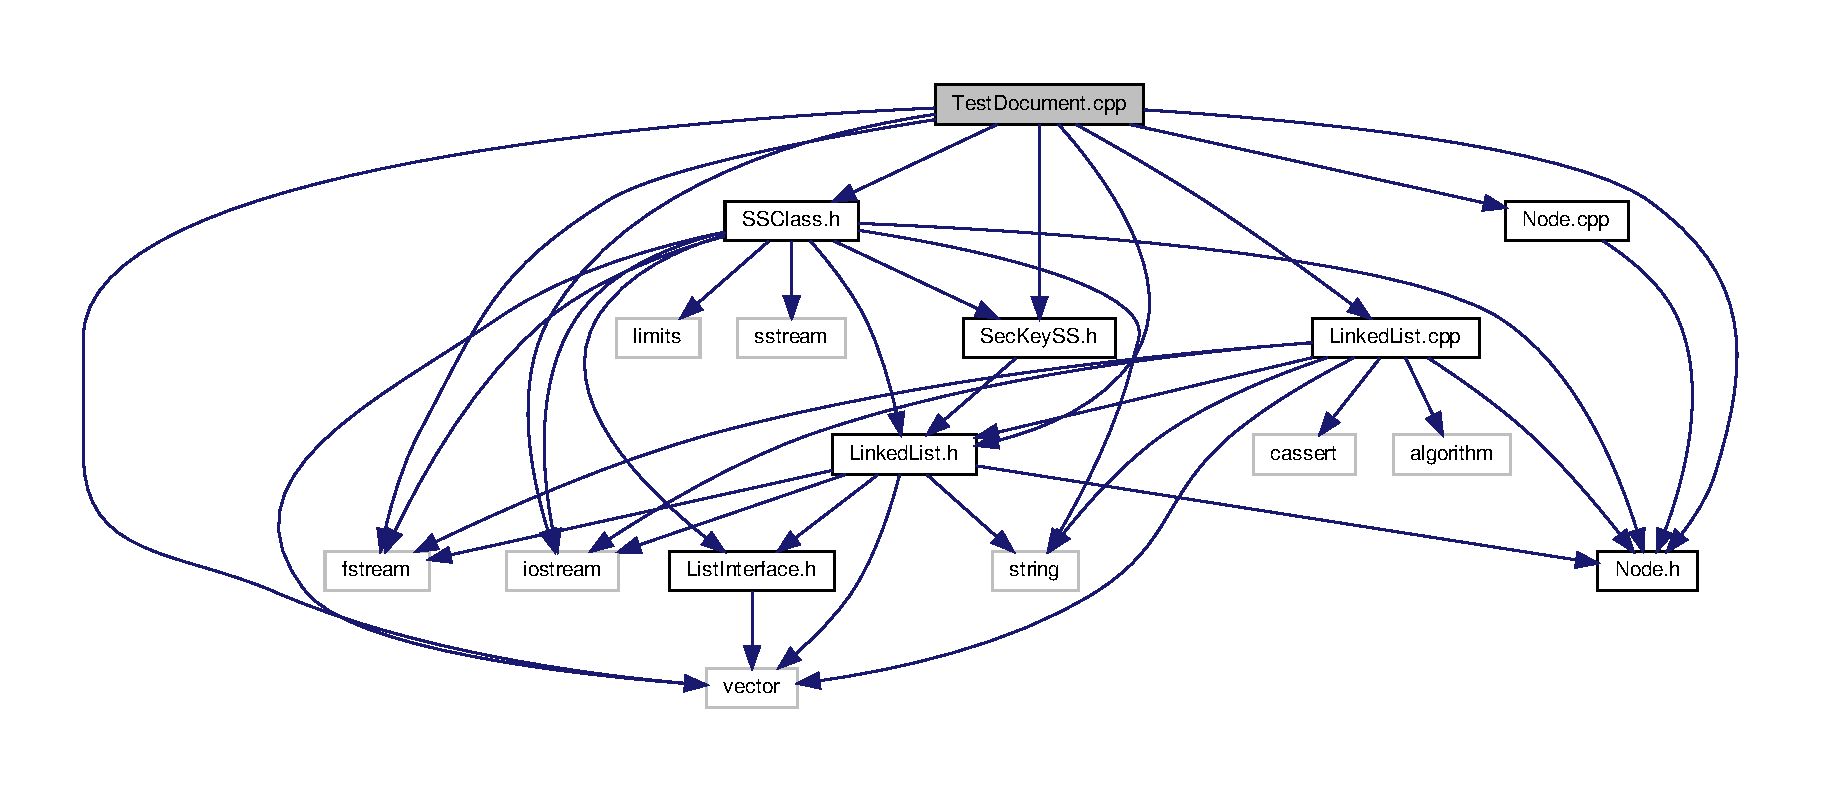
\includegraphics[width=350pt]{TestDocument_8cpp__incl}
\end{center}
\end{figure}
\subsection*{Functions}
\begin{DoxyCompactItemize}
\item 
void \hyperlink{TestDocument_8cpp_a23e4bdfe8835d4c21bff59dfd73e05f5}{menu} (uint8\+\_\+t \&)
\item 
int \hyperlink{TestDocument_8cpp_ae66f6b31b5ad750f1fe042a706a4e3d4}{main} ()
\end{DoxyCompactItemize}


\subsection{Function Documentation}
\mbox{\Hypertarget{TestDocument_8cpp_ae66f6b31b5ad750f1fe042a706a4e3d4}\label{TestDocument_8cpp_ae66f6b31b5ad750f1fe042a706a4e3d4}} 
\index{Test\+Document.\+cpp@{Test\+Document.\+cpp}!main@{main}}
\index{main@{main}!Test\+Document.\+cpp@{Test\+Document.\+cpp}}
\subsubsection{\texorpdfstring{main()}{main()}}
{\footnotesize\ttfamily int main (\begin{DoxyParamCaption}{ }\end{DoxyParamCaption})}



Definition at line \hyperlink{TestDocument_8cpp_source_l00017}{17} of file \hyperlink{TestDocument_8cpp_source}{Test\+Document.\+cpp}.

\mbox{\Hypertarget{TestDocument_8cpp_a23e4bdfe8835d4c21bff59dfd73e05f5}\label{TestDocument_8cpp_a23e4bdfe8835d4c21bff59dfd73e05f5}} 
\index{Test\+Document.\+cpp@{Test\+Document.\+cpp}!menu@{menu}}
\index{menu@{menu}!Test\+Document.\+cpp@{Test\+Document.\+cpp}}
\subsubsection{\texorpdfstring{menu()}{menu()}}
{\footnotesize\ttfamily void menu (\begin{DoxyParamCaption}\item[{uint8\+\_\+t \&}]{menu\+Selection }\end{DoxyParamCaption})}



Definition at line \hyperlink{TestDocument_8cpp_source_l00057}{57} of file \hyperlink{TestDocument_8cpp_source}{Test\+Document.\+cpp}.


\hypertarget{TestDocument_8cpp_source}{}\section{Test\+Document.\+cpp}

\begin{DoxyCode}
00001 \textcolor{preprocessor}{#include <fstream>}
00002 \textcolor{preprocessor}{#include <iostream>}
00003 \textcolor{preprocessor}{#include "\hyperlink{SSClass_8h}{SSClass.h}"}
00004 \textcolor{preprocessor}{#include <vector>}
00005 
00006 \textcolor{preprocessor}{#include "\hyperlink{LinkedList_8h}{LinkedList.h}"}
00007 \textcolor{preprocessor}{#include "\hyperlink{LinkedList_8cpp}{LinkedList.cpp}"}
00008 \textcolor{preprocessor}{#include "\hyperlink{Node_8h}{Node.h}"}
00009 \textcolor{preprocessor}{#include "\hyperlink{Node_8cpp}{Node.cpp}"}
00010 \textcolor{preprocessor}{#include "\hyperlink{SecKeySS_8h}{SecKeySS.h}"}
00011 
00012 \textcolor{keyword}{using namespace }\hyperlink{namespacestd}{std};
00013 
00014 \textcolor{comment}{// Function prototype for menu}
00015 \textcolor{keywordtype}{void} \hyperlink{TestDocument_8cpp_a23e4bdfe8835d4c21bff59dfd73e05f5}{menu}(uint8\_t &);
00016 
\Hypertarget{TestDocument_8cpp_source_l00017}\hyperlink{TestDocument_8cpp_ae66f6b31b5ad750f1fe042a706a4e3d4}{00017} \textcolor{keywordtype}{int} \hyperlink{TestDocument_8cpp_ae66f6b31b5ad750f1fe042a706a4e3d4}{main}()
00018 \{
00019     
00020     uint8\_t menuSelection = 9;  \textcolor{comment}{// allocates the memory for menu selection, and innitile to 0 to display
       menu}
00021 
00022     cout << \textcolor{stringliteral}{"\(\backslash\)n\(\backslash\)nWelcome to CSCI 331 SS Class Program: "} << endl;   \textcolor{comment}{// welcom message}
00023 
00024     \textcolor{comment}{// do while loop to call menu after every selection, and display menu when selection is 0}
00025     \textcolor{keywordflow}{do}
00026     \{
00027         \textcolor{keywordflow}{if}(menuSelection == 9)
00028         \{
00029             \textcolor{comment}{//Menu that will be displayed to the user.}
00030             cout << endl << endl;
00031             cout << \textcolor{stringliteral}{"*********************************************************"} << endl;
00032             cout << \textcolor{stringliteral}{"*                           Menu\(\backslash\)t\(\backslash\)t\(\backslash\)t*"} << endl;
00033             cout << \textcolor{stringliteral}{"*\(\backslash\)t0. \(\backslash\)tMenu  \(\backslash\)t\(\backslash\)t\(\backslash\)t\(\backslash\)t\(\backslash\)t*"} << endl;
00034             cout << \textcolor{stringliteral}{"*\(\backslash\)t1. \(\backslash\)tOpen file\(\backslash\)t\(\backslash\)t\(\backslash\)t*"} << endl;
00035             cout << \textcolor{stringliteral}{"*\(\backslash\)t2. \(\backslash\)tInsert  \(\backslash\)t\(\backslash\)t\(\backslash\)t\(\backslash\)t\(\backslash\)t*"} << endl;
00036             cout << \textcolor{stringliteral}{"*\(\backslash\)t3. \(\backslash\)tRemove \(\backslash\)t\(\backslash\)t\(\backslash\)t\(\backslash\)t\(\backslash\)t**"} << endl;
00037             cout << \textcolor{stringliteral}{"*\(\backslash\)t4. \(\backslash\)tModify \(\backslash\)t\(\backslash\)t\(\backslash\)t\(\backslash\)t\(\backslash\)t**"} << endl;
00038             cout << \textcolor{stringliteral}{"*\(\backslash\)t5. \(\backslash\)tDisplay recrod \(\backslash\)t\(\backslash\)t\(\backslash\)t\(\backslash\)t\(\backslash\)t**"} << endl;
00039             cout << \textcolor{stringliteral}{"*\(\backslash\)t6. \(\backslash\)tDisplay feild in recrod\(\backslash\)t\(\backslash\)t\(\backslash\)t\(\backslash\)t\(\backslash\)t*"} << endl;
00040             cout << \textcolor{stringliteral}{"*\(\backslash\)t7. \(\backslash\)tVerify \(\backslash\)t\(\backslash\)t\(\backslash\)t\(\backslash\)t\(\backslash\)t*"} << endl;
00041             cout << \textcolor{stringliteral}{"*\(\backslash\)t8. \(\backslash\)tRun Test Sequence\(\backslash\)t\(\backslash\)t\(\backslash\)t\(\backslash\)t\(\backslash\)t*"} << endl;
00042             cout << \textcolor{stringliteral}{"*\(\backslash\)t9. \(\backslash\)tSearch state \(\backslash\)t\(\backslash\)t\(\backslash\)t\(\backslash\)t\(\backslash\)t*"} << endl;
00043             cout << \textcolor{stringliteral}{"*\(\backslash\)t10. \(\backslash\)tQuit\(\backslash\)t\(\backslash\)t\(\backslash\)t\(\backslash\)t\(\backslash\)t*"} << endl;         
00044             cout << \textcolor{stringliteral}{"*********************************************************"} << endl;
00045             cout << endl << endl;
00046         \}
00047         
00048         \hyperlink{TestDocument_8cpp_a23e4bdfe8835d4c21bff59dfd73e05f5}{menu}(menuSelection);    \textcolor{comment}{// Calls menu function and passes menu selection}
00049 
00050     \}\textcolor{keywordflow}{while}(menuSelection != 10 );   \textcolor{comment}{// if selection is 10 quit the program}
00051 
00052     cout << \textcolor{stringliteral}{"Thank you for using SS Class program. Have a great day!!\(\backslash\)n"} << endl;   \textcolor{comment}{//good bye message}
00053 
00054     \textcolor{keywordflow}{return} 0;
00055 \}
00056 
\Hypertarget{TestDocument_8cpp_source_l00057}\hyperlink{TestDocument_8cpp_a23e4bdfe8835d4c21bff59dfd73e05f5}{00057} \textcolor{keywordtype}{void} \hyperlink{TestDocument_8cpp_a23e4bdfe8835d4c21bff59dfd73e05f5}{menu}(uint8\_t &menuSelection)
00058 \{
00059     \hyperlink{classSSClass}{SSClass} sequence;
00060     \textcolor{keywordtype}{string} file\_name;   \textcolor{comment}{// allocates memory for file name}
00061     \textcolor{keywordtype}{char} direction;
00062     \textcolor{keywordtype}{char} state;
00063     \textcolor{keywordtype}{string} zipCode;
00064     vector rrnVector;
00065 
00066     cout << \textcolor{stringliteral}{"Menu Selection: "};     \textcolor{comment}{// message to user  }
00067     cin >> menuSelection;           \textcolor{comment}{// takes in user input for menuSelection}
00068     cout << endl;                   
00069 
00070     \textcolor{keywordflow}{switch}(menuSelection)
00071     \{
00072         \textcolor{keywordflow}{case} 0: 
00073                 \textcolor{keywordflow}{break};
00074 
00075         \textcolor{keywordflow}{case} 1: cout << \textcolor{stringliteral}{"Enter a file name: "};
00076                 cin >> file\_name; cout << endl;
00077                 \textcolor{comment}{//sequence.openFile(file\_name); // TODO should param be a string or char* []?}
00078                 \textcolor{keywordflow}{break};
00079         
00080         \textcolor{keywordflow}{case} 2: cout << \textcolor{stringliteral}{"Insert: "};
00081                 \textcolor{comment}{//cin >> temp; cout << endl;}
00082                 \textcolor{comment}{//list.insert();    // TODO add param(s)}
00083                 \textcolor{keywordflow}{break};
00084         
00085         \textcolor{keywordflow}{case} 3: cout << \textcolor{stringliteral}{"remove: "};
00086                 \textcolor{comment}{//cin >> temp; cout << endl;}
00087                 \textcolor{comment}{//list.remove();    // TODO add param(s)}
00088                 \textcolor{keywordflow}{break};
00089 
00090         \textcolor{keywordflow}{case} 4: \textcolor{comment}{// TODO call modify function}
00091                 \textcolor{keywordflow}{break};
00092 
00093         \textcolor{keywordflow}{case} 5: \textcolor{comment}{// TODO call Display recrod function}
00094                 \textcolor{keywordflow}{break};
00095 
00096         \textcolor{keywordflow}{case} 6: \textcolor{comment}{// TODO call Display feild in recrod function}
00097             cout << \textcolor{stringliteral}{"Display field in record\(\backslash\)n"};
00098             cout << \textcolor{stringliteral}{"What is the zip code you would like to know the state and place name of?:"}
00099                 cin << zipCode; cout << endl;
00100             rrnVector = sequence.\hyperlink{classSSClass_a9df3598c000a6a5e9ef994d19196e69f}{search}(zipCode, 1);
00101             \textcolor{keywordflow}{for} (\textcolor{keywordtype}{int} i = 0; i < rrnVector.size(); i++) \{
00102                 cout << sequence.\hyperlink{classSSClass_ab0a8ea1af895df28359b5733bd920ef3}{returnLine}(rrnVector[i]);
00103             \}
00104 
00105                 \textcolor{keywordflow}{break};
00106 
00107         \textcolor{keywordflow}{case} 7: \textcolor{comment}{// TODO call Verify function}
00108                 \textcolor{keywordflow}{break};
00109 
00110         \textcolor{keywordflow}{case} 8: \textcolor{comment}{// TODO call Run Test Sequence function}
00111                 \textcolor{keywordflow}{break};
00112 
00113         \textcolor{keywordflow}{case} 9: \textcolor{comment}{// TODO call Search state function}
00114                 cout << \textcolor{stringliteral}{"enter direction N, E, S, or W: "};
00115                 cin >> direction; cout << endl;
00116                 cout << \textcolor{stringliteral}{"enter state"};
00117                 cin >> state; cout << endl;
00118 
00119                 \textcolor{keywordflow}{if} (direction == \textcolor{charliteral}{'N'} || direction == \textcolor{charliteral}{'S'} || direction == \textcolor{charliteral}{'E'} || direction == \textcolor{charliteral}{'W'})
00120                 \{
00121                     cout << sequence.\hyperlink{classSSClass_ab0a8ea1af895df28359b5733bd920ef3}{returnLine}(sequence.
      \hyperlink{classSSClass_ad03c99840c2946a2112f5f1942c287f2}{directionalSearch}(state, direction));
00122                 \}
00123 
00124                 \textcolor{keywordflow}{else}
00125                 \{
00126                     cout << direction << \textcolor{stringliteral}{" is not a valid response. please try again. "} << endl;
00127                 \}
00128                 \textcolor{keywordflow}{break};
00129 
00130         \textcolor{keywordflow}{case} 10: \textcolor{comment}{// quit}
00131                 \textcolor{keywordflow}{break};
00132 
00133         \textcolor{keywordflow}{default}: cout << \textcolor{stringliteral}{"****Please make a valid menu selection. ****"} << endl << endl; 
00134                 \textcolor{keywordflow}{break};
00135     \}
00136 \}
\end{DoxyCode}

%--- End generated contents ---

% Index
\backmatter
\newpage
\phantomsection
\clearemptydoublepage
\addcontentsline{toc}{chapter}{Index}
\printindex

\end{document}
